\documentclass[10pt,letterpaper]{article}
% Course manuscript with NeurIPS-style single-column typography.
% Course report: no conference submission, acceptance, or venue footer implied.
\usepackage[textwidth=6in,textheight=9.15in,top=.9in,headheight=12pt,headsep=20pt,footskip=26pt]{geometry}
\usepackage[T1]{fontenc}
\usepackage{mathptmx}
\usepackage{microtype}
\usepackage{amsmath,amssymb}
\usepackage{booktabs,tabularx,array}
\usepackage{enumitem}
\usepackage{xcolor}
\usepackage[hidelinks]{hyperref}
\usepackage{xurl}
\usepackage{upquote}
\usepackage[authoryear,round]{natbib}
\usepackage{caption}
\usepackage{flafter}
\usepackage{pgfplots}
\pgfplotsset{compat=1.18}
\usepgfplotslibrary{groupplots}
\definecolor{lassoblue}{HTML}{2563A6}
\definecolor{lassoorange}{HTML}{CF7A26}
\definecolor{lassogreen}{HTML}{258365}
\definecolor{lassopurple}{HTML}{805AB1}
\definecolor{lassopink}{HTML}{C34A76}
\pgfplotsset{every axis/.append style={
  axis line style={black!55},tick style={black!45},grid style={black!10},
  title style={font=\small\bfseries},tick label style={font=\scriptsize},
  label style={font=\small},legend style={font=\scriptsize,draw=none,fill=white},
  scaled ticks=false}}
\captionsetup{font=small,labelfont=bf,labelsep=period,skip=7pt}
\captionsetup[table]{position=top,skip=7pt}
\setlength{\parskip}{4.5pt}
\setlength{\parindent}{0pt}
\setlength{\emergencystretch}{1em}
\setlength{\parfillskip}{0pt plus 1fil}
\finalhyphendemerits=10000
\hyphenation{Tibshirani Daubechies Friedman Parikh Teboulle Boyd Wright Efron}
\setlength{\textfloatsep}{14pt plus 2pt minus 2pt}
\setlength{\floatsep}{12pt plus 2pt minus 2pt}
\setlength{\intextsep}{12pt plus 2pt minus 2pt}
\renewcommand{\arraystretch}{1.12}
\renewcommand{\topfraction}{.90}
\renewcommand{\bottomfraction}{.55}
\renewcommand{\textfraction}{.08}
\renewcommand{\floatpagefraction}{.80}
\setcounter{topnumber}{3}
\setcounter{bottomnumber}{2}
\setcounter{totalnumber}{4}
\widowpenalty=10000
\clubpenalty=10000
\raggedbottom
\makeatletter
\renewcommand{\normalsize}{\@setfontsize\normalsize{10}{11}\abovedisplayskip=7pt plus2pt minus3pt\belowdisplayskip=\abovedisplayskip}
\renewcommand{\small}{\@setfontsize\small{9}{10}}
\renewcommand{\footnotesize}{\@setfontsize\footnotesize{9}{10}}
\renewcommand{\scriptsize}{\@setfontsize\scriptsize{8}{9}}
\renewcommand{\section}{\@startsection{section}{1}{\z@}{-2ex plus-.5ex minus-.2ex}{1.2ex plus.2ex}{\fontsize{12}{14}\selectfont\bfseries\raggedright}}
\renewcommand{\subsection}{\@startsection{subsection}{2}{\z@}{-1.8ex plus-.3ex minus-.2ex}{.7ex plus.2ex}{\normalsize\bfseries\raggedright}}
\makeatother
\normalsize
\newcolumntype{Y}{>{\raggedright\arraybackslash}X}
\newcommand{\R}{\mathbb{R}}
\newcommand{\soft}{\mathcal{S}}
\begin{document}
\begin{center}
\hrule height4pt
\vspace{.18in}
{\fontsize{17}{20}\selectfont\bfseries Classical Optimization Algorithms\\for Lasso Regression\par}
\vspace{5pt}
{\fontsize{11}{13}\selectfont A Review and Empirical Comparison\par}
\vspace{.14in}
\hrule height1pt
\vspace{10pt}
{\bfseries COMP6704 Group Project --- Group 9\par}
{Convex Optimization\par}
\vspace{9pt}
\begin{minipage}[t]{.48\linewidth}\centering\small\setlength{\parskip}{0pt}
{\normalsize\bfseries CAI Yangxiao\textsuperscript{*}}\par
The Hong Kong Polytechnic University\par
Student ID: 26023041R\par
\href{mailto:26023041r@connect.polyu.hk}{26023041r@connect.polyu.hk}
\end{minipage}\hfill
\begin{minipage}[t]{.48\linewidth}\centering\small\setlength{\parskip}{0pt}
{\normalsize\bfseries XUE Pengyu\textsuperscript{*}}\par
The Hong Kong Polytechnic University\par
Student ID: 26022951R\par
\href{mailto:26022951r@connect.polyu.hk}{26022951r@connect.polyu.hk}
\end{minipage}\par
\vspace{8pt}
\begin{minipage}[t]{.48\linewidth}\centering\small\setlength{\parskip}{0pt}
{\normalsize\bfseries ZHANG Kejia\textsuperscript{*}}\par
The Hong Kong Polytechnic University\par
Student ID: 26049131R\par
\href{mailto:26049131r@connect.polyu.hk}{26049131r@connect.polyu.hk}
\end{minipage}\hfill
\begin{minipage}[t]{.48\linewidth}\centering\small\setlength{\parskip}{0pt}
{\normalsize\bfseries ZHOU Xiyu\textsuperscript{*}}\par
The Hong Kong Polytechnic University\par
Student ID: 26025265R\par
\href{mailto:26025265r@connect.polyu.hk}{26025265r@connect.polyu.hk}
\end{minipage}
\end{center}
\begingroup
\renewcommand{\thefootnote}{\ensuremath{*}}
\footnotetext[1]{All authors contributed equally and are listed in alphabetical order by surname.}
\endgroup
\vspace{4pt}
\begin{center}\fontsize{12}{14}\selectfont\bfseries Abstract\end{center}
\begin{list}{}{\setlength{\leftmargin}{.5in}\setlength{\rightmargin}{.5in}}
\item[]
Lasso regression combines squared loss with an $\ell_1$ penalty to learn sparse linear models. We review its convex formulation and compare three implemented solvers: ISTA, standard FISTA, and cyclic coordinate descent. A common proximal-gradient residual controls stopping accuracy on three synthetic instances, one fixed Diabetes split, and controlled correlation and dimension studies. The solvers reach nearly identical objectives and predictions, but their computational rankings depend on the design. ISTA is fastest on the original independent-feature instances and coordinate descent on Diabetes; FISTA becomes fastest on average at within-block correlation 0.99, with substantial variation. Penalty and coefficient analyses distinguish sparse selection from shrinkage error. The study relates theory to measured computation while documenting implementation costs, statistical limitations, and reproducibility.

\end{list}
\noindent\textbf{Code and data.}\footnote{Project repository: \textit{[GitHub URL to be supplied by Group 9 before submission]}. Reproduction instructions are given in Section~\ref{sec:reproducibility}.}
\vspace{3pt}
\section{Introduction and Literature Review}
Lasso adds an $\ell_1$ penalty to least-squares regression, shrinking coefficients and allowing exact zeros \citep{tibshirani1996}. It supports interpretable prediction and variable selection while retaining a convex objective. Nonsmoothness at zero makes its efficient solution an instructive optimization problem: global optimality follows from convexity, but computational cost depends on the update mechanism and data geometry.

We ask three questions: (i) how do ISTA, FISTA, and cyclic coordinate descent (CD) differ at a common stationarity tolerance; (ii) how do correlation and feature count change their measured efficiency; and (iii) how does the penalty affect prediction, sparsity, and coefficient shrinkage? The contribution is a reproducible comparison of classical methods, rather than a new algorithm. Fixed-penalty solver comparisons are kept separate from regularization sensitivity.

\subsection{Theoretical foundations and related work}
This focused narrative review covers convex squared-loss Lasso. Iterative thresholding \citep{daubechies2004} and the proximal framework \citep{parikh2014} explain ISTA; \citet{beck2009} establish FISTA's accelerated objective-error bound. Regression-specific coordinate updates appear in \citet{wu2008,friedman2010}, with convergence assumptions and coordinate-selection distinctions discussed by \citet{tseng2001,wright2015}. Table~\ref{tab:literature} organizes the relevant mechanisms.

Statistical and numerical guarantees answer different questions. Uniqueness controls coefficient agreement across accurate solvers \citep{tibshirani2013}; support recovery requires assumptions on the predictor structure \citep{zhao2006}. LARS provides solution-path context and the Diabetes example \citep{efron2004}, while related penalties, splitting, and safe screening clarify alternatives to the three benchmarked implementations.

\begin{center}\begin{minipage}{\linewidth}\captionsetup{type=table}\centering\small
\caption{Literature organized by mechanism and question.}\label{tab:literature}
\begin{tabular*}{\linewidth}{@{\extracolsep{\fill}}lll@{}}\toprule
\textbf{Mechanism / question} & \textbf{Reference} & \textbf{Key idea}\\\midrule
Penalty geometry & \citet{tibshirani1996} & $\ell_1$\\
Thresholding & \citet{daubechies2004} & $\soft_\tau$\\
Extrapolation & \citet{beck2009} & $O(k^{-2})$\\
Scalar minimization & \citet{wu2008} & $r^{(j)}$\\
Regression paths & \citet{friedman2010} & Warm starts\\
Convergence conditions & \citet{tseng2001} & Separability\\
Coordinate choice & \citet{wright2015} & Cyclic / random\\
Curvature-based steps & \citet{kim2007} & Barrier + Newton\\
Splitting & \citet{boyd2011} & ADMM\\
Variable elimination & \citet{ndiaye2017} & Safe region\\
\bottomrule\end{tabular*}
\end{minipage}\end{center}


\section{Problem Formulation and Motivation}
\subsection{Objective and preprocessing}
Write $X\in\R^{n\times d}$ for the training matrix, $y\in\R^n$ for centered responses, and $w\in\R^d$ for coefficients. With $\lambda>0$ controlling regularization, the squared-loss Lasso objective is
\begin{equation}
 F(w)=g(w)+h(w)
 =\frac{1}{2n}\|Xw-y\|_2^2+\lambda\|w\|_1,\qquad\lambda>0.
 \label{eq:objective}
\end{equation}
The loss measures fit and the penalty encourages sparse coefficients. All solvers use this normalization, so gradients, step sizes, and thresholds are directly comparable. Standardization matters because predictor units change coefficient magnitudes and the effective penalty.

Training means and population standard deviations center and scale features; training response means center the targets. Constant training features are removed. Test data use these training statistics, and predictions restore the response mean, giving an unpenalized intercept without test leakage. Synthetic coefficient comparisons undo feature scaling to recover original units.

\subsection{Convex formulations}
The constrained view of Lasso minimizes the loss over a norm ball:
\begin{equation}
 \min_w g(w)\quad\text{subject to}\quad \|w\|_1\leq t,\qquad t\geq0.
 \label{eq:constrained}
\end{equation}
For any minimizer $w^\star$ of Eq.~\eqref{eq:objective}, choosing $t=\|w^\star\|_1$ makes it optimal for Eq.~\eqref{eq:constrained}. A feasible point with smaller loss would also have a smaller penalized objective. Conversely, for $t>0$, strict feasibility at $w=0$ yields a constraint multiplier $\lambda\geq0$ and a corresponding penalized problem. The correspondence need not be one-to-one \citep{tibshirani1996,boyd2004}.

Introducing $u\in\R^d$ gives an exact reformulation of the penalized model:
\begin{equation}
 \min_{w,u}\ \frac{1}{2n}\|Xw-y\|_2^2+\lambda\sum_{j=1}^d u_j
 \quad\text{subject to}\quad -u\leq w\leq u.
 \label{eq:qp}
\end{equation}
The inequalities are componentwise. Because $\lambda>0$, an optimum has $u_j=|w_j|$; hence Eq.~\eqref{eq:qp} is an exact convex quadratic program \citep{boyd2004}. Our solvers operate directly on Eq.~\eqref{eq:objective}.

\subsection{Convexity, existence, and optimality}
The loss gradient supplies the fitting step in ISTA and FISTA. The Hessian is positive semidefinite because $a^\top X^\top Xa=\|Xa\|_2^2\geq0$ for every $a$, which proves convexity:
\begin{equation}
\nabla g(w)=\frac{X^\top(Xw-y)}{n},
\qquad \nabla^2g(w)=\frac{X^\top X}{n}\succeq0.
\label{eq:gradient}
\end{equation}
The $\ell_1$ norm is convex, so $F$ is convex. Since $\lambda>0$, $F$ is coercive and has a minimizer. Full column rank of $X$ gives strong convexity and a unique coefficient vector; it is sufficient, not necessary, for uniqueness \citep{tibshirani2013}. If coefficients are nonunique, optimal fitted values still agree, while active sets can differ.

The subgradient of $|u|$ at zero is $[-1,1]$. Applying this rule coordinate by coordinate gives the optimality condition below: the loss gradient must be balanced by a subgradient of the penalty.
\begin{equation}
0\in\nabla g(w^\star)+\lambda\partial\|w^\star\|_1.
\label{eq:optimality}
\end{equation}
The QP in Eq.~\eqref{eq:qp} is strictly feasible at $w=0$, $u=\mathbf{1}$, regardless of the column rank of $X$. Its Karush--Kuhn--Tucker (KKT) conditions characterize global optima and reduce to Eq.~\eqref{eq:optimality} after eliminating the auxiliary variables and multipliers \citep{boyd2004}.

The two cases are $\nabla_jg(w^\star)=-\lambda\operatorname{sign}(w_j^\star)$ for $w_j^\star\ne0$ and $|\nabla_jg(w^\star)|\leq\lambda$ for $w_j^\star=0$. The interval in the second case permits exact zeros. The same optimality condition gives a stationarity check that applies to all three solvers at a common accuracy \citep{parikh2014}.

\subsection{Why the penalty produces sparse coefficients}
The $\ell_1$ ball has corners on the coordinate axes, making zero coefficients compatible with a loss contour touching the constraint boundary \citep{tibshirani1996}. This geometry explains sparsity, not guaranteed recovery of the generating variables. Model-selection consistency requires additional predictor assumptions, such as the irrepresentable condition studied by \citet{zhao2006}; our finite-sample support checks are empirical observations.

An orthogonal design gives a direct algebraic example. If $X^\top X/n=I$, the quadratic loss separates into scalar terms. Writing $v=X^\top y/n$, each coefficient has the following closed-form solution:
\begin{equation}
w^\star=\soft_\lambda(v),\qquad
\soft_\tau(v)_j=\operatorname{sign}(v_j)\max\{|v_j|-\tau,0\}.
\label{eq:soft}
\end{equation}
For $v=(1.2,-0.4,0.1)$ and $\lambda=0.3$, the solution is $(0.9,-0.1,0)$. Figure~\ref{fig:soft} shows the zero interval and shrinkage outside it. For general designs, thresholding remains a building block: ISTA/FISTA apply it after a gradient step, and CD within a scalar minimization.

\begin{center}\begin{minipage}{\linewidth}\captionsetup{type=figure}\centering
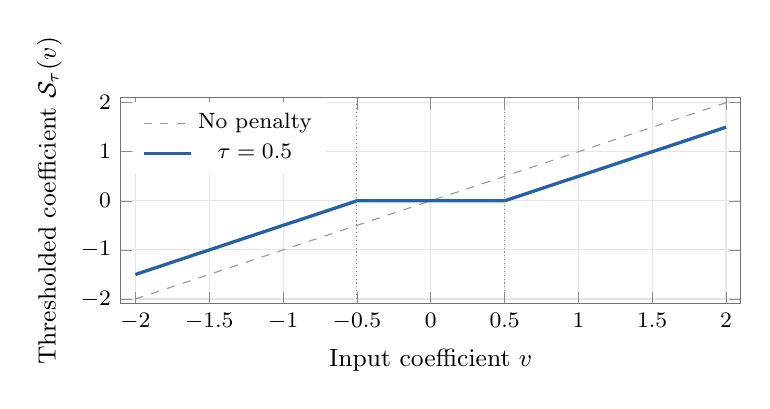
\begin{tikzpicture}
\begin{axis}[width=.78\linewidth,height=4.2cm,xmin=-2.1,xmax=2.1,ymin=-2.1,ymax=2.1,
 xlabel={Input coefficient $v$},ylabel={Thresholded coefficient $\soft_\tau(v)$},
 legend style={at={(.02,.98)},anchor=north west},grid=major]
\addplot[black!40,dashed] coordinates {(-2,-2)(2,2)};\addlegendentry{No penalty}
\addplot[lassoblue,very thick] coordinates {(-2,-1.5)(-.5,0)(.5,0)(2,1.5)};
\addlegendentry{$\tau=0.5$}
\addplot[black!45,densely dotted] coordinates {(-.5,-2)(-.5,2)};
\addplot[black!45,densely dotted] coordinates {(.5,-2)(.5,2)};
\end{axis}\end{tikzpicture}
\caption{Soft thresholding ($\tau=0.5$): zeros inside $[-\tau,\tau]$; shrinkage outside.}\label{fig:soft}
\end{minipage}\end{center}


\subsection{Related penalties: changing the model}
Table~\ref{tab:models} compares related convex estimators. Ridge stabilizes estimates under nonorthogonal predictors \citep{hoerl1970}; elastic net combines sparsity and grouped selection of correlated predictors \citep{zou2005}. These alternatives change the model, while our experiments fix the Lasso objective.

\begin{center}\begin{minipage}{\linewidth}\captionsetup{type=table}\centering\small
\caption{Related convex penalties; all use the loss $g(w)$ in Eq.~\eqref{eq:objective}.}\label{tab:models}
\begin{tabular*}{\linewidth}{@{\extracolsep{\fill}}llc@{}}\toprule
\textbf{Model} & \textbf{Penalty} & \textbf{Main distinction}\\\midrule
Ridge & $\tfrac{\alpha}{2}\|w\|_2^2$ & Quadratic shrinkage\\
Lasso & $\lambda\|w\|_1$ & Uniform thresholds\\
Elastic net & $\lambda\|w\|_1+\tfrac{\alpha}{2}\|w\|_2^2$ & Grouping\\
Adaptive Lasso & $\lambda\sum_j\omega_j|w_j|$ & Weighted thresholds\\
\bottomrule\end{tabular*}
\par\vspace{3pt}{\scriptsize $\alpha,\lambda>0$; fixed $\omega_j>0$.}
\end{minipage}\end{center}

Adaptive Lasso estimates weights from an initial fit \citep{zou2006}. With finite positive weights fixed, the objective is convex and the proximal thresholds become $\eta\lambda\omega_j$. Its statistical guarantees require assumptions on the initial estimator, design, and penalty sequence.

\section{Methodology: Algorithms and Computational Trade-offs}
Table~\ref{tab:taxonomy} compares the evaluation point, update, and dense cost per round. ISTA uses the current iterate, FISTA uses an extrapolated iterate, and coordinate descent uses the latest partial residual. A coordinate-descent round means a complete scan of all $d$ variables.


\begin{center}\begin{minipage}{\linewidth}\captionsetup{type=table}\centering\small
\caption{Update mechanisms.}\label{tab:taxonomy}
\begin{tabular*}{\linewidth}{@{\extracolsep{\fill}}lclc@{}}\toprule
\textbf{Method} & \textbf{Input} & \textbf{Update} & \textbf{Cost}\\\midrule
ISTA & $w^k$ & $\soft_{\lambda/L}(w^k-\nabla g(w^k)/L)$ & $O(nd)$\\
FISTA & $z^k$ & $\soft_{\lambda/L}(z^k-\nabla g(z^k)/L)$ & $O(nd)$\\
Cyclic CD & $r^{(j)}$ & Eq.~\eqref{eq:cd} & $O(nd)$\\
\bottomrule\end{tabular*}
\par\vspace{3pt}{\scriptsize $\eta=1/L$; CD: $d$ coordinates / sweep.}
\end{minipage}\end{center}


\subsection{ISTA}
The proximal subproblem separates across coordinates. The $\ell_1$ penalty can therefore be handled through scalar minimizations with closed-form solutions, giving the following vector operation:
\begin{equation}
\operatorname*{arg\,min}_u\left\{\frac12\|u-v\|_2^2+\tau\|u\|_1\right\}
=\soft_\tau(v).
\end{equation}
For $u>0$ or $u<0$, scalar differentiation yields $u=v-\tau$ or $u=v+\tau$; when $|v|\leq\tau$, zero satisfies the subgradient condition. These cases give Eq.~\eqref{eq:soft} \citep{parikh2014}.

The gradient of $g$ is Lipschitz continuous with constant $L=\|X\|_2^2/n$, where $\|X\|_2$ is the spectral norm. For $0<\eta\leq1/L$, the smooth loss has a quadratic upper bound at the current iterate. Minimizing this bound together with the penalty gives the next coefficient vector through the update
\begin{equation}
w^{k+1}=\soft_{\eta\lambda}\bigl(w^k-\eta\nabla g(w^k)\bigr).
\label{eq:ista}
\end{equation}
ISTA combines a fitting step with exact thresholding \citep{daubechies2004}. With the stated step size its objective is nonincreasing. Dense work is dominated by $Xw$ and $X^\top(Xw-y)$; a full Gram matrix is unnecessary. Its simplicity comes with a slower worst-case objective-error bound than FISTA.

\subsection{FISTA}
FISTA applies the proximal step to an extrapolated point \citep{beck2009}. Initialize $z^1=w^0$ and $t_1=1$, then use $\eta=1/L$. The sequence $t_k$ controls the contribution of the previous direction. Each round computes the coefficients before the next extrapolation:
\begin{align}
w^k&=\soft_{\eta\lambda}\bigl(z^k-\eta\nabla g(z^k)\bigr),\\
t_{k+1}&=\frac{1+\sqrt{1+4t_k^2}}{2},\\
z^{k+1}&=w^k+\frac{t_k-1}{t_{k+1}}(w^k-w^{k-1}), \qquad k\geq1.
\end{align}
The extrapolation uses the recent direction of movement. It requires extra vector operations and a previous iterate, while the dominant matrix-vector products remain the same as those in ISTA.

For convex composite objectives with a Lipschitz-continuous smooth gradient, an existing minimizer, exact proximal updates, and step size $1/L$, the standard bounds are
\begin{align}
F(w^k)-F^\star&\leq\frac{L\|w^0-w^\star\|_2^2}{2k}
&&\text{(ISTA)},\\
F(w^k)-F^\star&\leq\frac{2L\|w^0-w^\star\|_2^2}{(k+1)^2}
&&\text{(FISTA)}.
\label{eq:rates}
\end{align}
These are objective-error bounds, not coefficient-error or elapsed-time bounds. They describe a worst-case guarantee and do not imply that every FISTA iterate improves on ISTA. Standard FISTA can have a nonmonotone objective. Our comparison uses this standard version without restart or monotonicity modifications, so that the algorithm being evaluated is unambiguous.

\subsection{Cyclic coordinate descent}
Coordinate descent fixes all coefficients except one and minimizes the resulting scalar objective. Write $x_j$ for column $j$ of $X$ and use the latest available coefficients to define

\begin{equation}
r^{(j)}=y-\sum_{\ell\ne j}x_\ell w_\ell.
\end{equation}
The scalar objective contains a quadratic loss and an absolute-value penalty. Its solution uses soft thresholding, divided by the squared norm of the feature column to account for its scale:
\begin{equation}
\begin{gathered}
\min_u\frac{1}{2n}\|r^{(j)}-x_ju\|_2^2+\lambda|u|,\\
w_j\leftarrow
\frac{\soft_\lambda(x_j^\top r^{(j)}/n)}{\|x_j\|_2^2/n}.
\end{gathered}
\label{eq:cd}
\end{equation}
The denominator is one for centered, unit-variance columns. The general formula retains the dependence on feature scaling, as in the regression coordinate update of \citet{friedman2010}.

Maintain $r=y-Xw$ throughout the sweep. Before updating coordinate $j$, form $r^{(j)}=r+x_jw_j$; afterwards, set $r=r^{(j)}-x_jw_j$. Each coordinate costs $O(n)$ for dense data, and a sweep costs $O(nd)$. Updating the residual after every coefficient change avoids repeated full predictions.

Exact scalar minimization makes the objective nonincreasing without a global gradient step size. Regression-specific CD analyses support this structure \citep{wu2008,friedman2010}. Convergence theory uses the separability of $\|w\|_1$ and additional regularity assumptions \citep{tseng2001}; randomized coordinate rates cannot be transferred directly to our cyclic implementation \citep{wright2015}. We therefore assign no unconditional cyclic-CD rate.

\subsection{Broader solver families and possible extensions}
LARS--Lasso follows a piecewise-linear path \citep{efron2004}; pathwise CD reuses solutions at nearby penalties \citep{friedman2010}. Path computation answers a different computational question from our cold fixed-penalty solves. Interior-point methods use a quadratic-program reformulation and barrier Newton steps with more involved linear algebra \citep{kim2007}. ADMM splits the loss and penalty, alternating a regularized linear solve, thresholding, and a dual update; reusable factorization can offset setup cost \citep{boyd2011}.

Adaptive restart can reset unproductive momentum \citep{odonoghue2015}, while Gap Safe screening removes variables certified inactive through a dual-feasible region \citep{ndiaye2017}. Both are useful future comparisons, but neither is implemented here. A feasible primal--dual gap bounds objective suboptimality; our stopping residual instead measures stationarity.

\subsection{Strengths, weaknesses, and fair comparison}
Table~\ref{tab:tradeoffs} records monotonicity and objective-error bounds. ISTA and FISTA assume a convex objective, a Lipschitz-continuous smooth gradient, exact proximal updates, and a valid step size \citep{beck2009}. No universal rate is assigned to cyclic coordinate descent.


\begin{center}\begin{minipage}{\linewidth}\captionsetup{type=table}\centering\small
\caption{Monotonicity and objective-error bounds.}\label{tab:tradeoffs}
\begin{tabular*}{\linewidth}{@{\extracolsep{\fill}}lcccc@{}}\toprule
\textbf{Method} & $\mathbf{F_{k+1}\leq F_k}$ & \textbf{Bound} & \textbf{Step} & \textbf{State}\\\midrule
ISTA & $\checkmark$ & $O(k^{-1})$ & $1/L$ & ---\\
FISTA & --- & $O(k^{-2})$ & $1/L$ & $z,t$\\
Cyclic CD & $\checkmark$ & --- & --- & $r$\\
\bottomrule\end{tabular*}
\par\vspace{3pt}{\scriptsize $F_k=F(w^k)$; $\checkmark$: monotone; ---: no claim / n.a.}
\end{minipage}\end{center}


ISTA offers simple, monotone progress but can be slow along weak-curvature directions. FISTA improves the worst-case objective bound at the cost of extra state and potentially oscillatory progress. CD exploits exact scalar solves and residual reuse, but a Python coordinate loop can be costly. All three require $O(nd)$ dense work per vector update or complete CD sweep, with different constants; storing the dense data costs $O(nd)$, update state costs $O(n+d)$, and retaining a $K$-round history adds $O(K)$ storage.

A sweep contains $d$ scalar updates, so round counts alone do not compare equal work. We also report elapsed time, objectives, and a common stationarity measure. At a fixed objective, converged methods should agree on optimal values; coefficient agreement additionally depends on uniqueness.

\section{Experimental Design and Reproducibility}
\subsection{Data}
The original benchmark uses saved inputs and fixed splits (Table~\ref{tab:data}); controlled sensitivity studies are specified in Section~\ref{sec:extended}. Every solver receives identical training-standardized data.

\begin{center}\begin{minipage}{\linewidth}\captionsetup{type=table}\centering\small
\caption{Dataset sizes per instance.}\label{tab:data}
\begin{tabular*}{\linewidth}{@{\extracolsep{\fill}}lrrrr@{}}\toprule
\textbf{Input} & \textbf{Instances} & \textbf{$N$} & \textbf{$d$} & \textbf{Train / test}\\\midrule
Synthetic sparse regression & 3 & 300 & 50 & 240 / 60\\
Diabetes regression & 1 & 442 & 10 & 353 / 89\\
\bottomrule\end{tabular*}\end{minipage}\end{center}


Features are independent standard-normal draws. Only the first five coefficients are nonzero, with values $(2,-1.5,1,-2,1.5)$. The remaining 45 are zero. Responses satisfy $y=Xw_{\mathrm{true}}+\varepsilon$ with normal noise of standard deviation 0.5. Seeds 0, 1, and 2 define three independently generated instances.

Diabetes contains 442 observations, ten baseline predictors, and a continuous measure of disease progression one year later \citep{efron2004}. We use the raw files distributed with scikit-learn 1.9.1 and standardize them on the training split \citep{sklearn_data}. Unlike the synthetic instances, this dataset has no known generating coefficients or correct support set.

A separate NumPy generator permutes row indices with the recorded split seed. The first $\lceil0.2N\rceil$ rows form the test set. Split seeds are 0, 1, and 2 for the synthetic instances and zero for Diabetes. Saved split assignments and input hashes identify the observations used in the experiments.

\subsection{Common settings and stopping check}
{
Table~\ref{tab:settings} gives the settings fixed before measurement. The penalty scale comes from the transformed training inputs. A zero vector becomes optimal at the largest absolute feature--response inner product divided by sample size. This defines the training-dependent reference value\par}
\begin{equation}
\lambda_{\max}=\frac{\|X^\top y\|_\infty}{n}.
\end{equation}
Eq.~\eqref{eq:optimality} shows that $w=0$ is optimal when $\lambda\geq\lambda_{\max}$. The main comparison uses $\lambda=0.1\lambda_{\max}$. This choice provides a nontrivial sparse fit; it is not claimed to minimize prediction error.


\begin{center}\begin{minipage}{\linewidth}\captionsetup{type=table}\centering\small
\caption{Experimental settings.}\label{tab:settings}
\begin{tabular*}{\linewidth}{@{\extracolsep{\fill}}ll@{}}\toprule
\textbf{Setting} & \textbf{Value}\\\midrule
Initialization & $w^0=0$\\
Penalty & $\lambda/\lambda_{\max}=0.1$\\
ISTA / FISTA step & $\eta=1/L,\quad L=\|X\|_2^2/n$\\
CD order & $j=1,\ldots,d$\\
Stopping & $R\leq10^{-6}$\\
Maximum rounds & $10^4$\\
Timing & $5$ repeats; median\\
Penalty ratios & $\{0.01,\,0.1,\,0.5,\,1\}$ (CD)\\
\bottomrule\end{tabular*}
\end{minipage}\end{center}


A common stopping check is needed because small parameter changes do not necessarily imply comparable optimization accuracy. Define the proximal-gradient mapping and normalized residual
\begin{align}
G_L(w)&=L\left[w-\soft_{\lambda/L}
                  \left(w-\frac{\nabla g(w)}{L}\right)\right],\\
R(w)&=\frac{\|G_L(w)\|_\infty}
{\max\{1,\|X^\top y/n\|_\infty\}}.
\label{eq:residual}
\end{align}
The mapping is zero exactly when the optimality condition holds \citep{parikh2014}. Its norm measures stationarity; it does not certify an upper bound on objective error. We evaluate it after every vector update or CD sweep, at the returned coefficient vector rather than the FISTA extrapolation point. A run that reaches its iteration limit before meeting the threshold is marked as unconverged.

\subsection{Comparison and measurement}
We record objective and residual trajectories, complete rounds, elapsed time, test MSE, and nonzero counts. Timing includes solver-specific preparation, objective recording, and the shared residual check. Loading, preprocessing, shared spectral-norm calculation, and plotting are excluded. There is no Gram precomputation or screening. Each instance yields the median of five repetitions; synthetic summaries are means and sample standard deviations over three instance medians, whereas Diabetes has one fixed split.

For the penalty study, CD solves four prespecified ratios to the same tolerance. A coefficient is counted nonzero when $|w_j|>10^{-6}$ in standardized units. Test scores describe the selected settings; they are not used for penalty selection or an unbiased post-selection accuracy claim.

\subsection{Implementation validation}
An orthogonal design checks coefficient error against Eq.~\eqref{eq:soft}. A separate nonorthogonal synthetic-seed-0 check compares objectives and residuals with a tighter scikit-learn solve using centered inputs, $\texttt{alpha}=\lambda$, and no fitted intercept \citep{sklearn_data}. These checks precede timing and assess normalization and numerical correctness.

\subsection{Reproducing the recorded experiments}\label{sec:reproducibility}
From the package's \texttt{03\_Code\_and\_Results} directory, create a Python~3.12 environment, install the pinned dependencies, and run:
{\small
\begin{verbatim}
python -m pip install -r requirements.txt
python scripts/run_experiments.py --output results/reproduction-01
python scripts/run_extended_experiments.py --output results/extended-reproduction-01
\end{verbatim}
}
Use new output directories to preserve the recorded results. The package includes fixed input CSVs and splits, input hashes, optimizer code, source snapshots, configurations, coefficient arrays, traces, and raw timing CSVs. The extensions also save 24 actual NPZ inputs. The README distinguishes experiment reruns from plot-only refreshes; the report source embeds the plotted numerical data. Absolute times depend on the host, so reproduction should check convergence and numerical agreement before comparing runtime.

\section{Experimental Results and Analysis}
\subsection{Validation and execution}
Both implementation checks passed. The largest absolute coefficient error on the orthogonal instance was $1.11\times10^{-15}$. On synthetic seed 0, relative objective differences from the tighter scikit-learn reference were at most $1.57\times10^{-12}$; the reference residual was $1.54\times10^{-14}$. These checks support the implemented normalization and updates, but do not certify a general solver ranking.

All 60 main timing runs (four instances, three methods, five repetitions) and all 16 regularization runs reached $R\leq10^{-6}$. Execution used Python 3.12.14, NumPy 2.3.5, scikit-learn 1.9.1, and Matplotlib 3.11.2 on an arm64 macOS host, with detected numerical thread pools limited to one thread. Raw timings, histories, coefficients, input hashes, and environment versions are retained.

\subsection{Efficiency at a common tolerance}


\begin{center}\begin{minipage}{\linewidth}\captionsetup{type=table}\centering\small
\caption{Solver comparison at $\lambda/\lambda_{\max}=0.1$.}\label{tab:optimization_results}
\begin{tabular*}{\linewidth}{@{\extracolsep{\fill}}lrrrr@{}}\toprule
\textbf{Method} & \textbf{Time (ms)} & \textbf{Rounds} & \textbf{Final $F$} & \textbf{$R$ ($10^{-6}$)}\\\midrule
\multicolumn{5}{@{}l}{\textit{Synthetic: three instances}}\\[2pt]
ISTA & $\mathbf{0.389}\,{\pm}\,0.013$ & $24.7\,{\pm}\,0.6$ & $1.800\,{\pm}\,0.174$ & $0.71\,{\pm}\,0.16$\\
FISTA & $0.519\,{\pm}\,0.035$ & $30.7\,{\pm}\,2.3$ & $1.800\,{\pm}\,0.174$ & $0.53\,{\pm}\,0.30$\\
CD & $0.596\,{\pm}\,0.010$ & $5.0$ & $1.800\,{\pm}\,0.174$ & $0.14\,{\pm}\,0.17$\\
\midrule
\multicolumn{5}{@{}l}{\textit{Diabetes: fixed split}}\\[2pt]
ISTA & $1.419$ & $92.0$ & $1812.178$ & $0.99$\\
FISTA & $1.437$ & $85.0$ & $1812.178$ & $0.31$\\
CD & $\mathbf{0.530}$ & $14.0$ & $1812.178$ & $0.40$\\
\bottomrule\end{tabular*}\par\vspace{3pt}{\scriptsize $\mu\pm s$: three instances; $t=\mathrm{median}(5)$; \textbf{bold}: min. $t$.}\end{minipage}\end{center}


On the synthetic instances, ISTA used 24--25 updates, FISTA used 28--32, and CD used five sweeps. ISTA had the shortest measured time on all three instances. CD completed fewer sweeps but each sweep made 50 sequential scalar updates in a Python loop. ISTA and FISTA used NumPy matrix-vector operations. These timings are consistent with loop overhead affecting CD at this size, although loop overhead was not measured by timing the individual operations separately.

On Diabetes, CD required 14 sweeps and a median of 0.530 ms, compared with 92 updates and 1.419 ms for ISTA and 85 updates and 1.437 ms for FISTA. CD was fastest in this setting. ISTA and FISTA timing ranges overlapped: 1.326--1.438 ms and 1.357--1.450 ms, respectively. Their small median difference does not support a robust speed distinction between these vector methods.

\begin{center}\begin{minipage}{\linewidth}\captionsetup{type=figure}\centering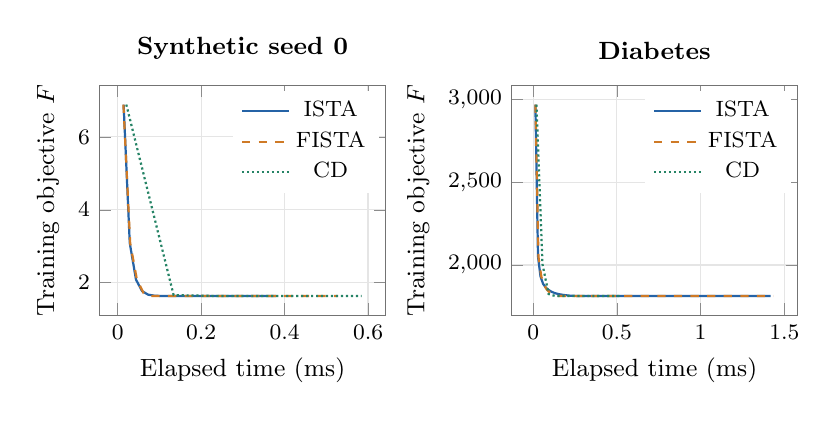
\begin{tikzpicture}
\begin{groupplot}[group style={group size=2 by 1,horizontal sep=1.6cm},width=.43\linewidth,height=4.5cm,
xlabel={Elapsed time (ms)},ylabel={Training objective $F$},tick label style={font=\scriptsize},label style={font=\small},
legend style={font=\scriptsize,at={(.98,.98)},anchor=north east},grid=major]
\nextgroupplot[title={Synthetic seed 0}]
\addplot[lassoblue,thick] coordinates {(0.014042,6.88816286) (0.02875,3.08833414) (0.043708,2.08334595) (0.058333,1.76622752) (0.072917,1.66970236) (0.08775,1.64264139) (0.102208,1.63474449) (0.11675,1.63240592) (0.131458,1.63170413) (0.145875,1.63149098) (0.160625,1.63142551) (0.175167,1.6314052) (0.19,1.63139884) (0.204458,1.63139683) (0.219208,1.63139618) (0.23375,1.63139598) (0.248292,1.63139591) (0.262875,1.63139589) (0.277417,1.63139588) (0.29175,1.63139588) (0.30625,1.63139588) (0.32075,1.63139588) (0.335125,1.63139588) (0.349833,1.63139588) (0.364167,1.63139588) (0.378958,1.63139588)};
\addlegendentry{ISTA}
\addplot[lassoorange,thick,dashed] coordinates {(0.013541,6.88816286) (0.02975,3.08833414) (0.045833,2.08334595) (0.061958,1.7112345) (0.078541,1.63547811) (0.094625,1.63244396) (0.111,1.63336655) (0.126916,1.63227743) (0.143083,1.63153593) (0.159375,1.6314073) (0.175333,1.6314265) (0.191666,1.63141931) (0.207541,1.63140285) (0.223708,1.63139667) (0.239791,1.63139653) (0.255708,1.63139667) (0.271833,1.63139626) (0.287708,1.63139596) (0.303666,1.6313959) (0.318791,1.63139591) (0.3345,1.6313959) (0.3505,1.63139589) (0.366458,1.63139588) (0.382625,1.63139588) (0.398416,1.63139588) (0.414791,1.63139588) (0.430875,1.63139588) (0.447041,1.63139588) (0.463083,1.63139588) (0.478916,1.63139588) (0.495125,1.63139588) (0.511083,1.63139588) (0.527208,1.63139588)};
\addlegendentry{FISTA}
\addplot[lassogreen,thick,densely dotted] coordinates {(0.0205,6.88816286) (0.133875,1.65801906) (0.247292,1.63145421) (0.360208,1.63139596) (0.4725,1.63139588) (0.584917,1.63139588)};
\addlegendentry{CD}
\nextgroupplot[title={Diabetes}]
\addplot[lassoblue,thick] coordinates {(0.013375,2969.82747) (0.029,2050.30114) (0.043959,1930.58044) (0.059084,1886.46583) (0.0745,1864.78393) (0.089917,1850.6147) (0.105417,1840.81119) (0.120167,1833.73688) (0.135459,1828.42813) (0.151167,1824.29919) (0.168542,1821.05043) (0.18475,1818.47128) (0.203,1816.3806) (0.218875,1814.66252) (0.234417,1813.86647) (0.249834,1813.3972) (0.264375,1813.07135) (0.279875,1812.83782) (0.295,1812.66842) (0.3105,1812.54449) (0.325209,1812.45314) (0.340625,1812.38535) (0.356,1812.33472) (0.371334,1812.29668) (0.385875,1812.26795) (0.401209,1812.24615) (0.416792,1812.22954) (0.432459,1812.21683) (0.446875,1812.20706) (0.462125,1812.19954) (0.477084,1812.19373) (0.492125,1812.18923) (0.507542,1812.18574) (0.52275,1812.18321) (0.538167,1812.18191) (0.553584,1812.18096) (0.569084,1812.18022) (0.584625,1812.17965) (0.599459,1812.1792) (0.61475,1812.17885) (0.629334,1812.17857) (0.643542,1812.17835) (0.658875,1812.17818) (0.673709,1812.17804) (0.68825,1812.17793) (0.703834,1812.17784) (0.719167,1812.17778) (0.734334,1812.17772) (0.748959,1812.17768) (0.764167,1812.17765) (0.778959,1812.17762) (0.79375,1812.1776) (0.809084,1812.17758) (0.824459,1812.17757) (0.840125,1812.17756) (0.854709,1812.17755) (0.87,1812.17754) (0.885375,1812.17754) (0.90075,1812.17753) (0.915459,1812.17753) (0.930709,1812.17753) (0.945584,1812.17752) (0.960125,1812.17752) (0.97525,1812.17752) (0.990792,1812.17752) (1.006209,1812.17752) (1.020917,1812.17752) (1.036459,1812.17752) (1.05175,1812.17752) (1.067042,1812.17752) (1.081875,1812.17752) (1.097292,1812.17752) (1.112167,1812.17752) (1.127417,1812.17752) (1.142917,1812.17752) (1.157834,1812.17752) (1.173459,1812.17752) (1.189292,1812.17752) (1.204542,1812.17752) (1.219917,1812.17752) (1.234709,1812.17752) (1.25025,1812.17752) (1.265625,1812.17752) (1.28125,1812.17752) (1.29575,1812.17752) (1.311209,1812.17752) (1.326917,1812.17752) (1.342292,1812.17752) (1.356917,1812.17752) (1.3725,1812.17752) (1.38825,1812.17752) (1.403709,1812.17752) (1.418417,1812.17752)};
\addlegendentry{ISTA}
\addplot[lassoorange,thick,dashed] coordinates {(0.01375,2969.82747) (0.0315,2050.30114) (0.048709,1930.58044) (0.065375,1877.93191) (0.082209,1850.5917) (0.098792,1833.75095) (0.115542,1823.4414) (0.1325,1816.67353) (0.149,1813.16557) (0.166,1812.49494) (0.182209,1812.44568) (0.198625,1812.35462) (0.215084,1812.27607) (0.231542,1812.25221) (0.248459,1812.23365) (0.264709,1812.21414) (0.281625,1812.20067) (0.2985,1812.19301) (0.315084,1812.18785) (0.332084,1812.18383) (0.348667,1812.18104) (0.3655,1812.17972) (0.382417,1812.17966) (0.399,1812.18014) (0.415709,1812.18041) (0.432625,1812.18009) (0.449459,1812.1793) (0.466375,1812.17841) (0.483042,1812.17778) (0.499584,1812.17753) (0.516875,1812.17759) (0.533584,1812.17776) (0.550375,1812.17789) (0.567084,1812.17792) (0.584042,1812.17785) (0.600542,1812.17773) (0.617167,1812.17762) (0.634209,1812.17755) (0.651,1812.17752) (0.667667,1812.17753) (0.684792,1812.17755) (0.7015,1812.17757) (0.718584,1812.17757) (0.735084,1812.17757) (0.751959,1812.17755) (0.768584,1812.17754) (0.785459,1812.17753) (0.802292,1812.17752) (0.818667,1812.17752) (0.835792,1812.17752) (0.852292,1812.17752) (0.869125,1812.17753) (0.886209,1812.17753) (0.902834,1812.17753) (0.919834,1812.17752) (0.936459,1812.17752) (0.95325,1812.17752) (0.970209,1812.17752) (0.986917,1812.17752) (1.003542,1812.17752) (1.020167,1812.17752) (1.037084,1812.17752) (1.053959,1812.17752) (1.070292,1812.17752) (1.086834,1812.17752) (1.103584,1812.17752) (1.120084,1812.17752) (1.137042,1812.17752) (1.153709,1812.17752) (1.1705,1812.17752) (1.186917,1812.17752) (1.203875,1812.17752) (1.220625,1812.17752) (1.237084,1812.17752) (1.253917,1812.17752) (1.270209,1812.17752) (1.286917,1812.17752) (1.304167,1812.17752) (1.320792,1812.17752) (1.337584,1812.17752) (1.353917,1812.17752) (1.370584,1812.17752) (1.387334,1812.17752) (1.403709,1812.17752) (1.42075,1812.17752) (1.436875,1812.17752)};
\addlegendentry{FISTA}
\addplot[lassogreen,thick,densely dotted] coordinates {(0.019666,2969.82747) (0.055708,2005.32301) (0.092,1824.81235) (0.1285,1813.4361) (0.164666,1812.45249) (0.200875,1812.23124) (0.237625,1812.18465) (0.27425,1812.17817) (0.310291,1812.17756) (0.346958,1812.17752) (0.383166,1812.17752) (0.42025,1812.17752) (0.456875,1812.17752) (0.493833,1812.17752) (0.529833,1812.17752)};
\addlegendentry{CD}
\end{groupplot}\end{tikzpicture}
\caption{Objective versus time; median-time repetition.}\label{fig:objective}\end{minipage}\end{center}

\begin{center}\begin{minipage}{\linewidth}\captionsetup{type=figure}\centering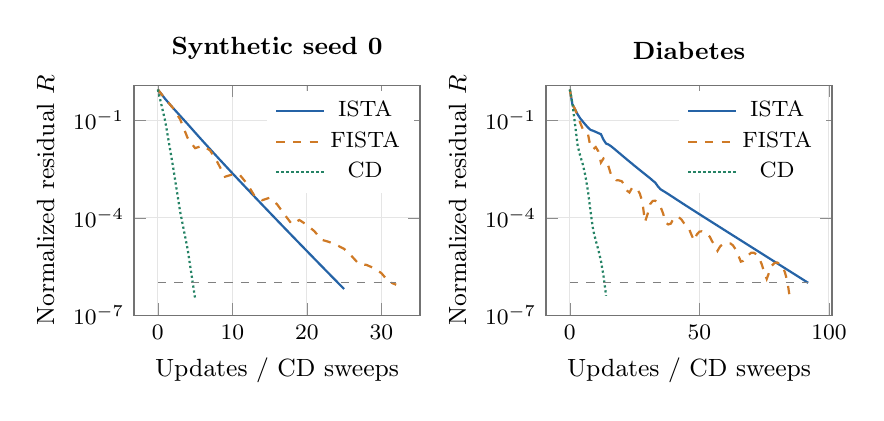
\begin{tikzpicture}
\begin{groupplot}[group style={group size=2 by 1,horizontal sep=1.6cm},width=.43\linewidth,height=4.5cm,
xlabel={Updates / CD sweeps},ylabel={Normalized residual $R$},tick label style={font=\scriptsize},label style={font=\small},
legend style={font=\scriptsize,at={(.98,.98)},anchor=north east},grid=major,ymode=log,ymin=1e-7,ymax=1.2]
\nextgroupplot[title={Synthetic seed 0}]
\addplot[lassoblue,thick] coordinates {(0,0.9) (1,0.455432794) (2,0.247670845) (3,0.138544221) (4,0.0773012068) (5,0.0425593593) (6,0.0236163258) (7,0.013194505) (8,0.00741544914) (9,0.00418884594) (10,0.00237662974) (11,0.00135357471) (12,0.000773465739) (13,0.000443260214) (14,0.000254675294) (15,0.000146657014) (16,8.46264203e-05) (17,4.89230007e-05) (18,2.83305828e-05) (19,1.64314636e-05) (20,9.54394086e-06) (21,5.55098381e-06) (22,3.2327263e-06) (23,1.88493123e-06) (24,1.10033356e-06) (25,6.43032941e-07)};
\addlegendentry{ISTA}
\addplot[lassoorange,thick,dashed] coordinates {(0,0.9) (1,0.455432794) (2,0.247670845) (3,0.107287112) (4,0.0286748138) (5,0.013988644) (6,0.0166127806) (7,0.0120377777) (8,0.00517466003) (9,0.00184270731) (10,0.00216520401) (11,0.00210331947) (12,0.00110672139) (13,0.000466002569) (14,0.000347819375) (15,0.000414355258) (16,0.000262697346) (17,0.00012704316) (18,6.36685352e-05) (19,8.57895853e-05) (20,6.06191939e-05) (21,3.91170211e-05) (22,2.11303593e-05) (23,1.80524117e-05) (24,1.45516654e-05) (25,1.10728532e-05) (26,6.70073133e-06) (27,3.75921441e-06) (28,3.55788106e-06) (29,2.82997587e-06) (30,1.98910065e-06) (31,1.081225e-06) (32,8.68686252e-07)};
\addlegendentry{FISTA}
\addplot[lassogreen,thick,densely dotted] coordinates {(0,0.9) (1,0.0930033112) (2,0.00424004028) (3,0.000151798178) (4,1.07123657e-05) (5,3.29790039e-07)};
\addlegendentry{CD}
\addplot[gray,dashed] coordinates {(0,1e-6)(32.0,1e-6)};
\nextgroupplot[title={Diabetes}]
\addplot[lassoblue,thick] coordinates {(0,0.9) (1,0.312844631) (2,0.222650828) (3,0.154780351) (4,0.116053875) (5,0.0923689123) (6,0.0745748373) (7,0.0605940121) (8,0.0511568099) (9,0.0481669247) (10,0.0443499139) (11,0.0407596221) (12,0.0379082544) (13,0.0254382722) (14,0.0194158551) (15,0.0179883867) (16,0.0158165098) (17,0.0136521792) (18,0.0117092801) (19,0.0100253969) (20,0.00858399326) (21,0.00735502818) (22,0.00630793048) (23,0.00541530384) (24,0.0046536038) (25,0.00400289048) (26,0.00344635359) (27,0.00296983055) (28,0.00256137938) (29,0.00221091653) (30,0.00190991454) (31,0.00165115069) (32,0.0014037249) (33,0.00120539424) (34,0.000931642495) (35,0.000758806932) (36,0.000677457246) (37,0.000606322474) (38,0.00053929133) (39,0.000478487984) (40,0.00042423346) (41,0.000376154421) (42,0.000333652941) (43,0.000296098395) (44,0.000262900007) (45,0.00023352928) (46,0.00020752229) (47,0.000184474616) (48,0.000164034215) (49,0.000145894313) (50,0.000129787016) (51,0.000115477817) (52,0.000102760951) (53,9.14554685e-05) (54,8.14019404e-05) (55,7.2459659e-05) (56,6.45042615e-05) (57,5.74256962e-05) (58,5.11264758e-05) (59,4.55201677e-05) (60,4.05300851e-05) (61,3.60881466e-05) (62,3.21338803e-05) (63,2.86135505e-05) (64,2.54793908e-05) (65,2.26889284e-05) (66,2.02043885e-05) (67,1.7992168e-05) (68,1.60223695e-05) (69,1.42683892e-05) (70,1.27065512e-05) (71,1.13157835e-05) (72,1.00773296e-05) (73,8.97449338e-06) (74,7.99241179e-06) (75,7.1178529e-06) (76,6.3390365e-06) (77,5.64547439e-06) (78,5.02782846e-06) (79,4.47778431e-06) (80,3.98793891e-06) (81,3.5517005e-06) (82,3.16319965e-06) (83,2.81720999e-06) (84,2.50907767e-06) (85,2.23465865e-06) (86,1.99026273e-06) (87,1.77260387e-06) (88,1.57875586e-06) (89,1.40611292e-06) (90,1.25235457e-06) (91,1.11541436e-06) (92,9.9345208e-07)};
\addlegendentry{ISTA}
\addplot[lassoorange,thick,dashed] coordinates {(0,0.9) (1,0.312844631) (2,0.222650828) (3,0.13604825) (4,0.0854274238) (5,0.0540496603) (6,0.0431792404) (7,0.0380406496) (8,0.0148292564) (9,0.0129669057) (10,0.0151378103) (11,0.0111515318) (12,0.0050608895) (13,0.0067431841) (14,0.00579191077) (15,0.00367275051) (16,0.00200573574) (17,0.00179423963) (18,0.00144324851) (19,0.00142309985) (20,0.00134502114) (21,0.00105895738) (22,0.000696115654) (23,0.000602771851) (24,0.000830771642) (25,0.000875049425) (26,0.000767574817) (27,0.000560963147) (28,0.000311929386) (29,7.53418206e-05) (30,0.000129044606) (31,0.00026476) (32,0.000331788757) (33,0.000336640796) (34,0.000293684136) (35,0.000220841131) (36,0.000135826334) (37,7.14098962e-05) (38,6.2395776e-05) (39,6.64911337e-05) (40,9.67707025e-05) (41,0.000108334938) (42,0.000104721915) (43,9.03217949e-05) (44,6.95251322e-05) (45,5.77670008e-05) (46,4.61016881e-05) (47,2.93377798e-05) (48,1.97294214e-05) (49,3.05521857e-05) (50,3.75006312e-05) (51,3.85707228e-05) (52,3.50875129e-05) (53,3.1542831e-05) (54,2.62341786e-05) (55,1.8444674e-05) (56,1.40556446e-05) (57,9.60896146e-06) (58,1.31146818e-05) (59,1.53480857e-05) (60,1.53426486e-05) (61,1.67752404e-05) (62,1.62466069e-05) (63,1.40504817e-05) (64,1.06262972e-05) (65,7.05070175e-06) (66,4.47358841e-06) (67,4.74525363e-06) (68,5.53942917e-06) (69,7.24506371e-06) (70,8.37745355e-06) (71,8.41892983e-06) (72,7.51274995e-06) (73,5.89103407e-06) (74,3.83594558e-06) (75,2.17187394e-06) (76,1.31275347e-06) (77,2.15538817e-06) (78,3.39426179e-06) (79,4.07629939e-06) (80,4.20555847e-06) (81,3.84792564e-06) (82,3.11436048e-06) (83,2.14152063e-06) (84,1.07244817e-06) (85,3.06545108e-07)};
\addlegendentry{FISTA}
\addplot[lassogreen,thick,densely dotted] coordinates {(0,0.9) (1,0.327877931) (2,0.0775597041) (3,0.0170256008) (4,0.00817497355) (5,0.00445160408) (6,0.00197713935) (7,0.000662787183) (8,0.000156902603) (9,4.21225636e-05) (10,1.99724439e-05) (11,1.0396302e-05) (12,4.73637475e-06) (13,1.62027709e-06) (14,3.96129418e-07)};
\addlegendentry{CD}
\addplot[gray,dashed] coordinates {(0,1e-6)(92.0,1e-6)};
\end{groupplot}\end{tikzpicture}
\caption{Residual versus rounds. Dashed line: $R=10^{-6}$.}\label{fig:stationarity}\end{minipage}\end{center}

{
Figure~\ref{fig:stationarity} shows oscillations in FISTA's residual and a smoother decrease for ISTA. Acceleration did not reduce the synthetic update count at this threshold. Eq.~\eqref{eq:rates} bounds worst-case objective error, whereas the stopping rule concerns an instance's proximal-gradient residual. Initial objective reduction alone therefore cannot determine time to the declared tolerance (Figure~\ref{fig:objective}). These observations concern standard FISTA; restart variants need a separate comparison.\par}

The shared spectral-norm calculation took 0.278--0.714 ms for synthetic instances and 3.070 ms for Diabetes. It is excluded from Table~\ref{tab:optimization_results} but would matter in an end-to-end application at these sizes. CD does not need $L$ for its scalar update; the common residual check does. These timings depend on the recorded input sizes, the solver and monitoring implementations, and the machine.


\subsection{What the timing repetitions establish}
The five timings in Figure~\ref{fig:timing} show disjoint ranges favoring ISTA on each original synthetic instance and CD on Diabetes. ISTA/FISTA ranges overlap on Diabetes, so their small median difference is inconclusive. Five short repetitions support descriptive comparison, not a significance claim. A five-sweep, 50-feature CD run contains 250 scalar updates; its round count cannot be read as an equal-cost speedup over 25 vector updates.

\begin{center}\begin{minipage}{\linewidth}\captionsetup{type=figure}\centering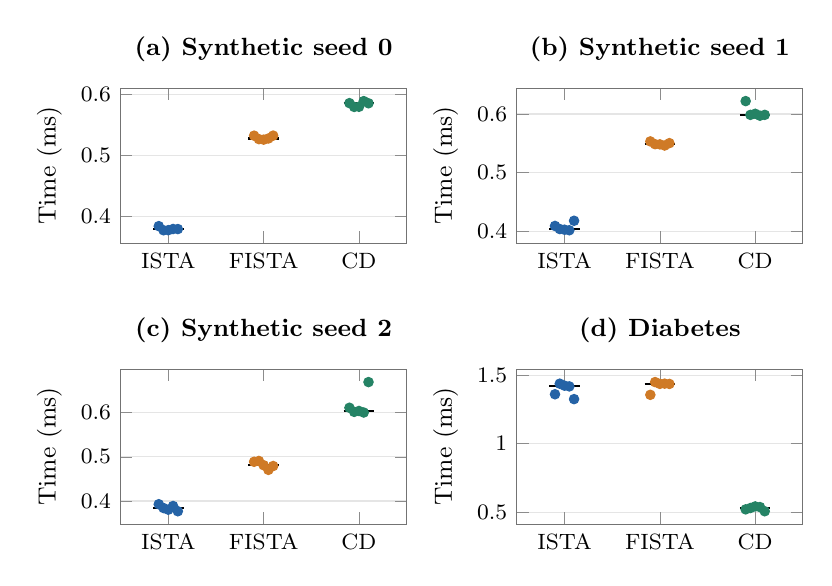
\begin{tikzpicture}
\begin{groupplot}[group style={group size=2 by 2,horizontal sep=1.4cm,vertical sep=1.6cm},
width=.43\linewidth,height=3.55cm,xmin=.5,xmax=3.5,xtick={1,2,3},xticklabels={ISTA,FISTA,CD},ylabel={Time (ms)},ymajorgrids=true]
\nextgroupplot[title={(a) Synthetic seed 0}]
\addplot[only marks,mark=*,mark size=1.7pt,lassoblue] coordinates {(0.900,0.383792) (0.950,0.377042) (1.000,0.377167) (1.050,0.379125) (1.100,0.379)};
\addplot[black,thick] coordinates {(0.84,0.379)(1.16,0.379)};
\addplot[only marks,mark=*,mark size=1.7pt,lassoorange] coordinates {(1.900,0.531958) (1.950,0.526291) (2.000,0.525417) (2.050,0.527333) (2.100,0.532042)};
\addplot[black,thick] coordinates {(1.84,0.527333)(2.16,0.527333)};
\addplot[only marks,mark=*,mark size=1.7pt,lassogreen] coordinates {(2.900,0.585208) (2.950,0.579) (3.000,0.579209) (3.050,0.588542) (3.100,0.584958)};
\addplot[black,thick] coordinates {(2.84,0.584958)(3.16,0.584958)};
\nextgroupplot[title={(b) Synthetic seed 1}]
\addplot[only marks,mark=*,mark size=1.7pt,lassoblue] coordinates {(0.900,0.409417) (0.950,0.404125) (1.000,0.403) (1.050,0.402042) (1.100,0.418208)};
\addplot[black,thick] coordinates {(0.84,0.404125)(1.16,0.404125)};
\addplot[only marks,mark=*,mark size=1.7pt,lassoorange] coordinates {(1.900,0.553375) (1.950,0.548625) (2.000,0.548333) (2.050,0.546333) (2.100,0.550417)};
\addplot[black,thick] coordinates {(1.84,0.548625)(2.16,0.548625)};
\addplot[only marks,mark=*,mark size=1.7pt,lassogreen] coordinates {(2.900,0.622) (2.950,0.598542) (3.000,0.600417) (3.050,0.597125) (3.100,0.598584)};
\addplot[black,thick] coordinates {(2.84,0.598584)(3.16,0.598584)};
\nextgroupplot[title={(c) Synthetic seed 2}]
\addplot[only marks,mark=*,mark size=1.7pt,lassoblue] coordinates {(0.900,0.392667) (0.950,0.384042) (1.000,0.380333) (1.050,0.388625) (1.100,0.376792)};
\addplot[black,thick] coordinates {(0.84,0.384042)(1.16,0.384042)};
\addplot[only marks,mark=*,mark size=1.7pt,lassoorange] coordinates {(1.900,0.488708) (1.950,0.490542) (2.000,0.480916) (2.050,0.470417) (2.100,0.479125)};
\addplot[black,thick] coordinates {(1.84,0.480916)(2.16,0.480916)};
\addplot[only marks,mark=*,mark size=1.7pt,lassogreen] coordinates {(2.900,0.610959) (2.950,0.601625) (3.000,0.603666) (3.050,0.600166) (3.100,0.669042)};
\addplot[black,thick] coordinates {(2.84,0.603666)(3.16,0.603666)};
\nextgroupplot[title={(d) Diabetes}]
\addplot[only marks,mark=*,mark size=1.7pt,lassoblue] coordinates {(0.900,1.361) (0.950,1.438292) (1.000,1.423791) (1.050,1.418584) (1.100,1.325584)};
\addplot[black,thick] coordinates {(0.84,1.418584)(1.16,1.418584)};
\addplot[only marks,mark=*,mark size=1.7pt,lassoorange] coordinates {(1.900,1.356958) (1.950,1.450042) (2.000,1.436917) (2.050,1.438584) (2.100,1.4365)};
\addplot[black,thick] coordinates {(1.84,1.436917)(2.16,1.436917)};
\addplot[only marks,mark=*,mark size=1.7pt,lassogreen] coordinates {(2.900,0.520042) (2.950,0.529875) (3.000,0.5415) (3.050,0.53675) (3.100,0.506209)};
\addplot[black,thick] coordinates {(2.84,0.529875)(3.16,0.529875)};
\end{groupplot}\end{tikzpicture}
\caption{Timing repetitions ($n=5$). Black bars: medians.}\label{fig:timing}\end{minipage}\end{center}

\subsection{Prediction and sparsity at the fixed penalty}


\begin{center}\begin{minipage}{\linewidth}\captionsetup{type=table}\centering\small
\caption{Prediction at $\lambda/\lambda_{\max}=0.1$.}\label{tab:prediction_results}
\begin{tabular*}{\linewidth}{@{\extracolsep{\fill}}lrr@{}}\toprule
\textbf{Method} & \textbf{Test MSE} & \textbf{Nonzero}\\\midrule
\multicolumn{3}{@{}l}{\textit{Synthetic: three instances}}\\[2pt]
ISTA & $0.396\,{\pm}\,0.139$ & $5$\\
FISTA & $0.396\,{\pm}\,0.139$ & $5$\\
CD & $0.396\,{\pm}\,0.139$ & $5$\\
\midrule
\multicolumn{3}{@{}l}{\textit{Diabetes: fixed split}}\\[2pt]
ISTA & $2966.935$ & $5$\\
FISTA & $2966.936$ & $5$\\
CD & $2966.937$ & $5$\\
\bottomrule\end{tabular*}\par\vspace{3pt}{\scriptsize $\mu\pm s$: three instances; nonzero: $|w_j|>10^{-6}$.}\end{minipage}\end{center}


{
The methods produced nearly identical objectives and prediction errors, retaining five coefficients on every instance. Diabetes MSE differences are below 0.002 on a scale near 2967 and do not establish a predictive advantage for any optimizer. Synthetic fits selected the generating variables, with magnitudes shrunk toward zero. The selected count on Diabetes cannot be assessed as recovery accuracy because its true support and generating coefficients are unknown.\par}


\subsection{Support recovery and shrinkage are different}
{
Figure~\ref{fig:coefficients} separates selection from magnitude estimation. All three synthetic CD fits retain the five generating coefficients and set the 45 inactive coefficients to zero. The active coefficient means are
\[ (1.801,-1.260,0.736,-1.810,1.287), \]
all closer to zero than their generating values. Their mean absolute error is $0.221\pm0.025$ across instances. Selecting the correct variables therefore does not remove the shrinkage error in their fitted coefficients, even when every active variable is retained.\par}

The Diabetes solution retains sex, bmi, bp, s3, and s5 on the fixed split. Signs and magnitudes describe a standardized fit; they do not establish causal effects or stable selection across splits. The synthetic panel compares fitted coefficients with the generating values in original units. The Diabetes panel compares predictors through their fitted standardized coefficients.


\begin{center}\begin{minipage}{\linewidth}\captionsetup{type=figure}\centering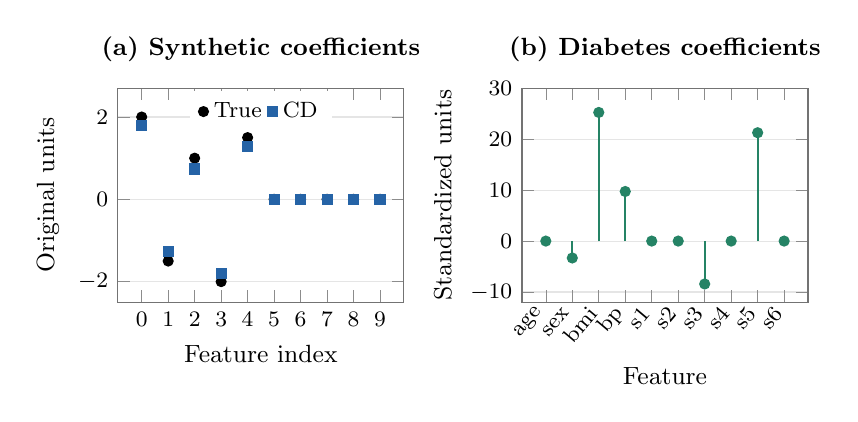
\begin{tikzpicture}
\begin{groupplot}[group style={group size=2 by 1,horizontal sep=1.5cm},width=.43\linewidth,height=4.3cm,
ymajorgrids=true,xtick={0,1,2,3,4,5,6,7,8,9}]
\nextgroupplot[title={(a) Synthetic coefficients},ylabel={Original units},xlabel={Feature index},ymin=-2.5,ymax=2.7,
legend style={at={(.5,.99)},anchor=north,legend columns=2}]
\addplot[black,only marks,mark=*,mark size=1.8pt] coordinates {(0,2.0) (1,-1.5) (2,1.0) (3,-2.0) (4,1.5) (5,0.0) (6,0.0) (7,0.0) (8,0.0) (9,0.0)};
\addlegendentry{True}
\addplot[lassoblue,only marks,mark=square*,mark size=1.8pt,error bars/.cd,y dir=both,y explicit] coordinates {(0,1.80100799) +- (0,0.0550045038) (1,-1.25970297) +- (0,0.035459667) (2,0.735873303) +- (0,0.0447481833) (3,-1.81046151) +- (0,0.0155839725) (4,1.28670574) +- (0,0.0187076477) (5,0) +- (0,0) (6,0) +- (0,0) (7,0) +- (0,0) (8,0) +- (0,0) (9,0) +- (0,0)};
\addlegendentry{CD}
\nextgroupplot[title={(b) Diabetes coefficients},ylabel={Standardized units},xlabel={Feature},
xticklabels={age,sex,bmi,bp,s1,s2,s3,s4,s5,s6},x tick label style={rotate=50,anchor=east},ymin=-12,ymax=30]
\addplot[lassogreen,ycomb,mark=*,mark size=1.6pt,thick] coordinates {(0,0) (1,-3.31495464) (2,25.2401022) (3,9.72941732) (4,-0) (5,-0) (6,-8.4190648) (7,0) (8,21.2607552) (9,0)};
\end{groupplot}\end{tikzpicture}
\caption{CD coefficients. Left: synthetic mean $\pm$ SD (original units); right: Diabetes (standardized units).}\label{fig:coefficients}\end{minipage}\end{center}

\subsection{Regularization effects}


\begin{center}\begin{minipage}{\linewidth}\captionsetup{type=table}\centering\small
\caption{Regularization study (CD).}\label{tab:penalty_results}
\begin{tabular*}{\linewidth}{@{\extracolsep{\fill}}crr@{}}\toprule
\textbf{$\lambda/\lambda_{\max}$} & \textbf{Test MSE} & \textbf{Nonzero}\\\midrule
\multicolumn{3}{@{}l}{\textit{Synthetic: three instances}}\\[2pt]
0.01 & $0.236\,{\pm}\,0.033$ & $22.3\,{\pm}\,3.5$\\
0.1 & $0.396\,{\pm}\,0.139$ & $5.0$\\
0.5 & $5.506\,{\pm}\,1.021$ & $4.3\,{\pm}\,0.6$\\
1 & $11.945\,{\pm}\,1.311$ & $0.0$\\
\midrule
\multicolumn{3}{@{}l}{\textit{Diabetes: fixed split}}\\[2pt]
0.01 & $2912.647$ & $8.0$\\
0.1 & $2966.937$ & $5.0$\\
0.5 & $3837.820$ & $2.0$\\
1 & $5893.048$ & $0.0$\\
\bottomrule\end{tabular*}\par\vspace{3pt}{\scriptsize $\mu\pm s$: three instances; nonzero: $|w_j|>10^{-6}$.}\end{minipage}\end{center}

\begin{center}\begin{minipage}{\linewidth}\captionsetup{type=figure}\centering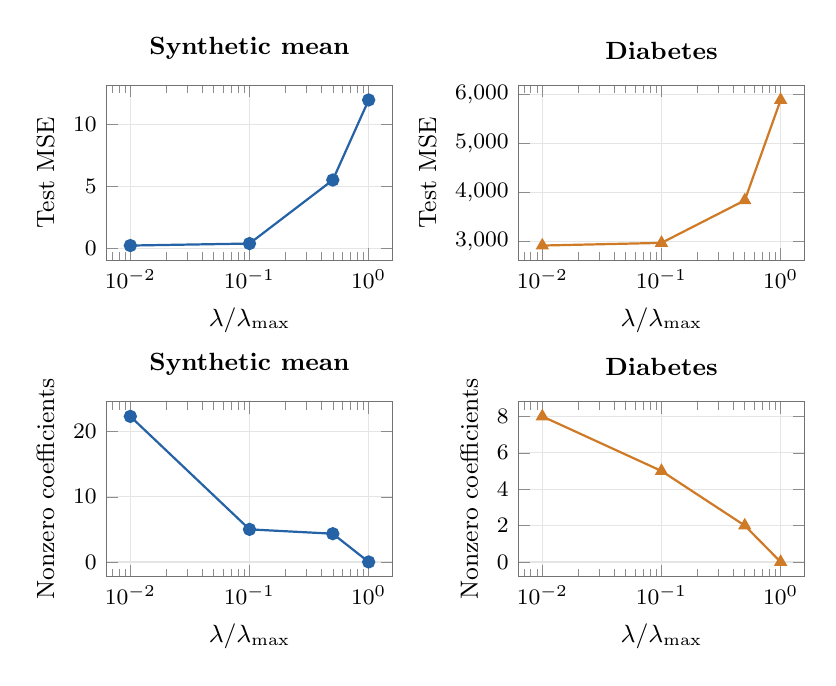
\begin{tikzpicture}
\begin{groupplot}[group style={group size=2 by 2,horizontal sep=1.6cm,vertical sep=1.8cm},width=.43\linewidth,height=3.8cm,xmode=log,
xlabel={$\lambda/\lambda_{\max}$},tick label style={font=\scriptsize},label style={font=\small},grid=major]
\nextgroupplot[title={Synthetic mean},ylabel={Test MSE}]
\addplot[lassoblue,mark=*,thick] coordinates {(0.01,0.235958863) (0.1,0.395982019) (0.5,5.50575318) (1.0,11.9445806)};
\nextgroupplot[title={Diabetes},ylabel={Test MSE}]
\addplot[lassoorange,mark=triangle*,thick] coordinates {(0.01,2912.6475) (0.1,2966.93661) (0.5,3837.82032) (1.0,5893.04764)};
\nextgroupplot[title={Synthetic mean},ylabel={Nonzero coefficients}]
\addplot[lassoblue,mark=*,thick] coordinates {(0.01,22.3333333) (0.1,5) (0.5,4.33333333) (1.0,0)};
\nextgroupplot[title={Diabetes},ylabel={Nonzero coefficients}]
\addplot[lassoorange,mark=triangle*,thick] coordinates {(0.01,8) (0.1,5) (0.5,2) (1.0,0)};
\end{groupplot}\end{tikzpicture}
\caption{Test MSE and selected variables versus penalty; synthetic means over three instances.}\label{fig:regularization}\end{minipage}\end{center}

Increasing the penalty reduced selected variables in these cases. For synthetic data, the mean count fell from 22.3 at ratio 0.01 to five at ratio 0.1, while mean test MSE rose from 0.2360 to 0.3960. The stronger penalty produced a smaller model without the lowest average prediction error. Individual errors were not strictly monotone: seed 1 had slightly lower MSE at 0.1 than at 0.01. At ratio 0.5, mean MSE rose to 5.5058, consistent with increased shrinkage bias.

For Diabetes, the selected count decreased from eight to five to two as the ratio increased from 0.01 to 0.1 to 0.5, and test MSE increased. At ratio 1, both datasets returned zero coefficients at initialization, as predicted by the optimality condition. Predictions then equal the training response mean. This fit--sparsity trade-off concerns the model and penalty, not superiority of CD as a predictor.


% BEGIN EXTENDED EXPERIMENTS
\subsection{Controlled correlation and dimension studies}\label{sec:extended}
The original benchmark is small and mostly well conditioned. To test whether its ordering persists, we vary within-block feature correlation and then feature count. The correlation study uses 600 observations and 60 features in blocks of ten. For feature $j$ in block $b$, independent standard-normal draws give
\begin{equation}
 x_j=\sqrt{\rho}\,z_b+\sqrt{1-\rho}\,z_j,
 \qquad \rho\in\{0,0.5,0.9,0.99\}.
 \label{eq:block-correlation}
\end{equation}
The first five coefficients are $(2,-1.5,1,-2,1.5)$, and noise has standard deviation 0.5. Seeds 10--12 share underlying random draws, noise, and a 480/120 split across correlation levels. The dimension study uses independent features, 1,000 observations, an 800/200 split, and $d\in\{50,100,300,600\}$. Within each seed, smaller designs use prefixes of the same 600-column matrix and the same response vector.

Both studies retain zero initialization, $\lambda=0.1\lambda_{\max}$, $R\leq10^{-6}$, and the 10,000-round limit. Each instance has five interleaved timings; reported means and sample standard deviations describe three instance medians. Solver time includes monitoring but excludes the shared spectral calculation. Thread settings are requested before importing the numerical libraries. These timings form a separate run and are not pooled with the original benchmark.

All 360 timed solves converge. The largest relative objective spread between solvers on the same problem is $8.61\times10^{-11}$. This check supports comparison at the stated stationarity tolerance; it does not make $R$ an objective-error bound. Actual inputs, splits, code snapshots, settings, and complete traces are retained with the new results.

\begin{center}\begin{minipage}{\linewidth}\captionsetup{type=table}\centering\small
\caption{Correlation study: condition number and solver time (ms).}\label{tab:correlation}
\begin{tabular*}{\linewidth}{@{\extracolsep{\fill}}@{}lrrrr@{}}\toprule
$\rho$ & $\kappa$ & ISTA & FISTA & Cyclic CD\\\midrule
0 & $4.1$ & \textbf{$0.360\,{\pm}\,0.010$} & $0.521\,{\pm}\,0.043$ & $0.762\,{\pm}\,0.107$\\
0.5 & $28.8$ & \textbf{$3.236\,{\pm}\,0.223$} & $3.782\,{\pm}\,0.208$ & $3.318\,{\pm}\,0.321$\\
0.9 & $230.3$ & $21.667\,{\pm}\,1.026$ & $16.876\,{\pm}\,1.160$ & \textbf{$16.443\,{\pm}\,1.622$}\\
0.99 & $2492.8$ & $154.599\,{\pm}\,10.491$ & \textbf{$19.862\,{\pm}\,18.153$} & $62.507\,{\pm}\,8.707$\\
\bottomrule\end{tabular*}\par\vspace{3pt}{\scriptsize $\mu\pm s$: three instance medians; $\kappa$: mean full-Gram condition number.}\end{minipage}\end{center}

At $\rho=0$, ISTA takes $0.360\pm0.010$ ms. At $\rho=0.99$, its mean time rises to 154.599 ms, while FISTA takes $19.862\pm18.153$ ms and CD takes $62.507\pm8.707$ ms. Acceleration has a measured advantage in this highly correlated setting, although the three FISTA instances vary widely. At $\rho=0.5$, the ISTA and CD means are close; the measurements do not establish a precise ranking between them.

The mean condition number $\kappa(X^\top X/n)$ grows from 4.1 to 2492.8. Greater correlation creates weak-curvature directions, which can slow fixed-step progress. The selected support and penalty scale also change, so this full-design condition number is a diagnostic rather than a complete prediction of solver time. The recorded $\rho=0.99$ trace shows FISTA reaching the threshold sooner despite residual oscillations; smooth progress and fast stopping are different properties.

\begin{center}\begin{minipage}{\linewidth}\captionsetup{type=figure}\centering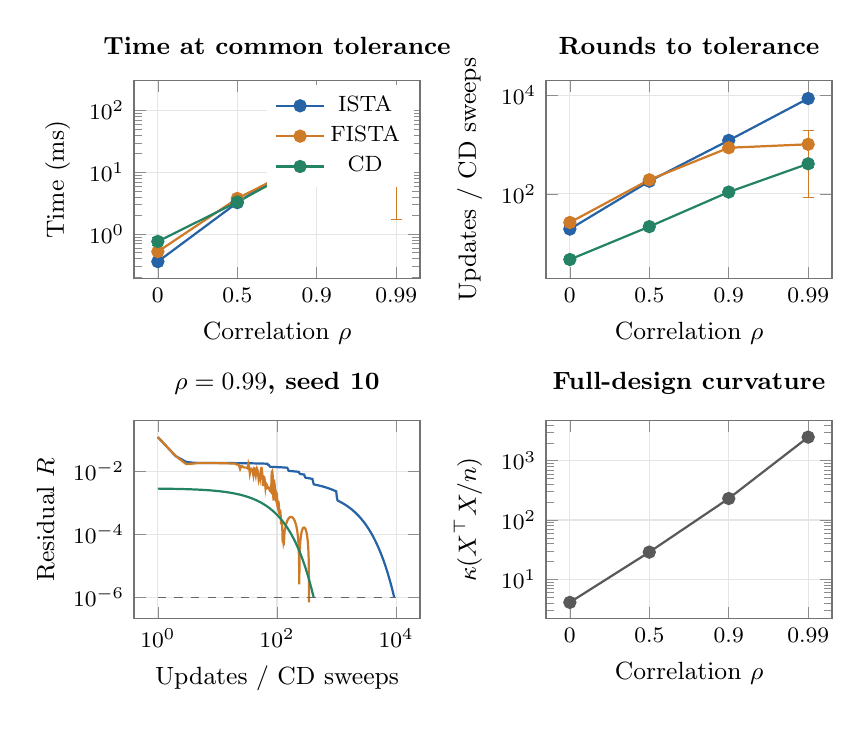
\begin{tikzpicture}
\begin{groupplot}[group style={group size=2 by 2,horizontal sep=1.6cm,vertical sep=1.8cm},width=.43\linewidth,height=4.1cm,grid=major]
\nextgroupplot[title={Time at common tolerance},ymode=log,xtick={0,1,2,3},xticklabels={0,0.5,0.9,0.99},xlabel={Correlation $\rho$},ylabel={Time (ms)}]
\addplot[lassoblue,thick,mark=*,error bars/.cd,y dir=both,y explicit] coordinates {(0,0.35959733) +- (0,0.0098867031) (1,3.2356527) +- (0,0.22294983) (2,21.667319) +- (0,1.0257483) (3,154.59856) +- (0,10.490784)};
\addlegendentry{ISTA}
\addplot[lassoorange,thick,mark=*,error bars/.cd,y dir=both,y explicit] coordinates {(0,0.52122233) +- (0,0.042503427) (1,3.781736) +- (0,0.20814939) (2,16.875542) +- (0,1.1598679) (3,19.861861) +- (0,18.152867)};
\addlegendentry{FISTA}
\addplot[lassogreen,thick,mark=*,error bars/.cd,y dir=both,y explicit] coordinates {(0,0.76218067) +- (0,0.10724638) (1,3.3184583) +- (0,0.32116801) (2,16.443153) +- (0,1.6221975) (3,62.507361) +- (0,8.7066784)};
\addlegendentry{CD}
\nextgroupplot[title={Rounds to tolerance},ymode=log,xtick={0,1,2,3},xticklabels={0,0.5,0.9,0.99},xlabel={Correlation $\rho$},ylabel={Updates / CD sweeps}]
\addplot[lassoblue,thick,mark=*,error bars/.cd,y dir=both,y explicit] coordinates {(0,19.333333) +- (0,1.1547005) (1,180.66667) +- (0,13.576941) (2,1214.3333) +- (0,71.90503) (3,8600.3333) +- (0,582.37817)};
\addplot[lassoorange,thick,mark=*,error bars/.cd,y dir=both,y explicit] coordinates {(0,26.333333) +- (0,2.8867513) (1,193.33333) +- (0,13.650397) (2,862.33333) +- (0,66.515662) (3,1013) +- (0,929.23248)};
\addplot[lassogreen,thick,mark=*,error bars/.cd,y dir=both,y explicit] coordinates {(0,4.6666667) +- (0,0.57735027) (1,21.666667) +- (0,2.081666) (2,109) +- (0,10.148892) (3,408) +- (0,58.103356)};
\nextgroupplot[title={$\rho=0.99$, seed 10},xmode=log,ymode=log,xlabel={Updates / CD sweeps},ylabel={Residual $R$},legend style={at={(.02,.98)},anchor=north west}]
\addplot[lassoblue,thick] coordinates {(1,0.11889077) (2,0.029682136) (3,0.019480915) (4,0.01830148) (5,0.018152246) (6,0.018120663) (7,0.018102528) (8,0.018085942) (9,0.018069546) (10,0.018053185) (11,0.018036841) (12,0.018020512) (13,0.018004198) (14,0.0179879) (15,0.017971616) (16,0.017955347) (17,0.017939093) (18,0.017922854) (19,0.017906629) (20,0.01789042) (21,0.017874225) (22,0.017858046) (23,0.017841881) (24,0.01782573) (25,0.017809595) (26,0.017793474) (27,0.017777368) (28,0.017761277) (29,0.017745201) (30,0.017729139) (31,0.017713092) (32,0.01769706) (33,0.017681042) (34,0.017665039) (35,0.017649051) (36,0.017633077) (37,0.017617118) (38,0.017601173) (39,0.017585243) (40,0.017569328) (41,0.017553427) (42,0.017537541) (43,0.017521669) (44,0.017505812) (45,0.017489969) (47,0.017458328) (48,0.017442528) (49,0.017426743) (50,0.017410973) (52,0.017379476) (53,0.017363749) (55,0.017332338) (56,0.017316654) (58,0.017285329) (59,0.017269688) (61,0.017238449) (62,0.017222851) (64,0.017191697) (66,0.017160601) (67,0.017145074) (69,0.017114063) (71,0.015667415) (73,0.015504725) (75,0.014326741) (77,0.013695555) (79,0.01362011) (81,0.01359184) (83,0.013567609) (85,0.01354376) (87,0.013519983) (90,0.013484399) (92,0.013460729) (95,0.013425303) (97,0.013401738) (100,0.013366469) (102,0.013343008) (105,0.013307895) (108,0.013272876) (111,0.01323795) (114,0.013203117) (117,0.013168376) (120,0.013133728) (123,0.013099172) (126,0.013064708) (130,0.013018899) (133,0.012984649) (137,0.012939123) (140,0.012905085) (144,0.012859842) (148,0.012814759) (152,0.011703947) (156,0.010281655) (160,0.010117094) (164,0.01007416) (169,0.010028047) (173,0.0099915426) (178,0.0099461082) (183,0.0099008822) (187,0.0098648504) (192,0.0098199964) (197,0.0097753477) (203,0.0097220389) (208,0.0096778386) (214,0.0096250652) (219,0.0095813087) (225,0.0095290653) (231,0.0094771087) (237,0.0086097687) (244,0.0080865666) (250,0.0080330787) (257,0.0079797288) (264,0.0079269576) (271,0.0078745386) (278,0.0078224661) (285,0.0077707375) (293,0.0066748645) (301,0.0061747776) (309,0.0061156408) (317,0.0060700675) (326,0.006019644) (334,0.0059751852) (343,0.0059255614) (352,0.0058763495) (362,0.0058221484) (372,0.0057684469) (381,0.0057205389) (392,0.0056625243) (402,0.0046846601) (413,0.0038184467) (424,0.0037539929) (435,0.0037165063) (447,0.0036769844) (459,0.0036379117) (471,0.0035992549) (483,0.0035610087) (496,0.0035200336) (510,0.0034764335) (523,0.0034364313) (537,0.0033938664) (552,0.0033488458) (566,0.0033073654) (581,0.0032634919) (597,0.0032173346) (613,0.0031718299) (629,0.0031269685) (646,0.0030799981) (663,0.003033733) (681,0.0029855034) (699,0.0029380403) (718,0.0028887584) (737,0.0028403029) (757,0.0027901746) (777,0.0027409306) (798,0.0026901593) (819,0.0026403281) (841,0.0025891133) (863,0.0025388916) (886,0.002487428) (910,0.0024348384) (934,0.0023833602) (959,0.0023308936) (985,0.0022775528) (1011,0.0014496432) (1038,0.0011692888) (1066,0.001140272) (1095,0.001112237) (1124,0.0010848964) (1154,0.00105732) (1185,0.0010295606) (1216,0.00100253) (1249,0.00097453485) (1282,0.00094732148) (1316,0.00092007804) (1352,0.00089208553) (1388,0.00086494466) (1425,0.00083791009) (1463,0.00081102417) (1502,0.0007843275) (1542,0.00075785891) (1583,0.00073165536) (1626,0.0007051464) (1669,0.00067959791) (1714,0.00065385179) (1759,0.00062908105) (1806,0.00060421073) (1855,0.00057932839) (1904,0.00055547074) (1955,0.00053168219) (2007,0.00050847582) (2061,0.00048544837) (2116,0.00046306618) (2173,0.0004409584) (2231,0.00041954588) (2290,0.00039883069) (2352,0.0003781634) (2414,0.00035856708) (2479,0.000339112) (2545,0.00032043739) (2613,0.00030227188) (2683,0.00028464716) (2755,0.00026759039) (2828,0.0002513399) (2904,0.00023546924) (2981,0.00022041148) (3061,0.0002057861) (3143,0.00019180169) (3227,0.00017846102) (3313,0.00016576347) (3402,0.00015357345) (3493,0.00014203585) (3586,0.00013113976) (3682,0.0001207682) (3780,0.00011102616) (3881,0.00010180753) (3985,9.3114281e-05) (4091,8.5017285e-05) (4201,7.7358361e-05) (4313,7.0268687e-05) (4428,6.3664632e-05) (4547,5.7483568e-05) (4668,5.1813598e-05) (4793,4.654284e-05) (4921,4.1700746e-05) (5053,3.7234357e-05) (5188,3.3160854e-05) (5326,2.9457059e-05) (5469,2.6054901e-05) (5615,2.2986417e-05) (5765,2.020981e-05) (5919,1.7707705e-05) (6077,1.5462204e-05) (6239,1.3455184e-05) (6406,1.1658541e-05) (6577,1.0067182e-05) (6753,8.6558147e-06) (6934,7.4104463e-06) (7119,6.322515e-06) (7309,5.3712051e-06) (7505,4.5395964e-06) (7705,3.8235946e-06) (7911,3.2039821e-06) (8122,2.6732814e-06) (8340,2.2171251e-06) (8562,1.8325035e-06) (8791,1.5055331e-06) (9026,1.2305506e-06) (9268,9.997687e-07)};
\addplot[lassoorange,thick] coordinates {(1,0.11889077) (2,0.029682136) (3,0.016606685) (4,0.017313008) (5,0.018057979) (6,0.018120734) (7,0.018047402) (8,0.017990655) (9,0.017943599) (10,0.01789353) (11,0.017838441) (12,0.017778999) (13,0.017715548) (14,0.017648136) (15,0.017576781) (16,0.017501517) (17,0.017422388) (18,0.017339439) (19,0.017252715) (20,0.017162262) (21,0.016104606) (22,0.016071383) (23,0.015196525) (24,0.011671942) (25,0.014175602) (26,0.014196611) (27,0.013493179) (28,0.013032884) (29,0.012894913) (30,0.012870424) (31,0.012822471) (32,0.012260817) (33,0.016933713) (34,0.013548209) (35,0.0084695091) (36,0.011139213) (37,0.011656022) (38,0.010777178) (39,0.0097082583) (40,0.0075986678) (41,0.01233716) (42,0.012064608) (43,0.0092813656) (44,0.0073815225) (45,0.010148733) (46,0.012045468) (47,0.0109293) (48,0.0083604038) (49,0.0057972687) (50,0.0071114037) (51,0.0075298577) (52,0.0060692046) (53,0.0085689437) (54,0.012297577) (55,0.012499615) (56,0.010182304) (57,0.0067135402) (58,0.0033506621) (59,0.0056061585) (60,0.006615668) (61,0.0064387263) (62,0.0054641109) (63,0.0041750876) (64,0.0030165055) (65,0.0037158915) (66,0.003953423) (67,0.0037900976) (68,0.0033750349) (69,0.0028797098) (70,0.0029060045) (71,0.0030847164) (72,0.0030983867) (73,0.002976651) (74,0.0027763295) (75,0.0025583351) (76,0.0023703245) (77,0.0023421839) (78,0.0023056085) (79,0.0022234604) (80,0.0028136758) (81,0.0071373869) (82,0.00949621) (83,0.0098728534) (84,0.008604616) (85,0.0062504579) (86,0.0034464441) (87,0.0011665706) (88,0.0032014593) (89,0.0043107445) (90,0.0044605451) (91,0.0038815478) (92,0.0029310106) (93,0.0019612378) (94,0.0026278467) (95,0.0013888509) (96,0.0012735916) (97,0.0017944313) (98,0.0020080943) (99,0.0019340178) (100,0.001638764) (101,0.0012147104) (102,0.00075848316) (103,0.00070691335) (104,0.00095343457) (105,0.001065874) (106,0.0010467657) (107,0.00092151866) (108,0.00072932865) (109,0.00051347414) (110,0.00040333293) (111,0.00051376292) (112,0.00056608767) (113,0.00055859492) (114,0.00050058641) (115,0.00040853657) (116,0.00030174649) (117,0.00020675457) (118,0.00025116924) (119,0.0002707139) (120,0.00026329549) (121,0.00023208672) (122,0.00018392196) (123,0.00012736194) (124,7.0835535e-05) (125,7.276922e-05) (126,7.583908e-05) (127,6.6943769e-05) (128,5.6877022e-05) (129,6.1712143e-05) (130,6.1270101e-05) (131,5.9442573e-05) (132,7.7423774e-05) (133,0.00010291667) (134,0.0001224413) (135,0.0001361854) (136,0.00014525315) (137,0.00015128991) (138,0.00015608448) (139,0.00016665232) (140,0.0001840093) (141,0.00019847362) (142,0.00021001745) (143,0.00021906428) (144,0.00022632611) (145,0.00023262112) (146,0.00023985707) (147,0.00025167358) (148,0.00026198893) (149,0.00027073739) (150,0.00027807371) (151,0.00028430322) (152,0.00028979894) (153,0.00029492272) (154,0.00030249633) (155,0.00030932465) (156,0.00031523283) (157,0.0003202739) (158,0.00032457829) (159,0.00032831638) (160,0.00033166123) (161,0.00033569203) (162,0.00033952414) (163,0.00034275464) (164,0.00034540076) (165,0.000347519) (166,0.00034918835) (167,0.00035049283) (168,0.00035182082) (169,0.00035305418) (170,0.00035385434) (171,0.00035422756) (172,0.00035419985) (173,0.00035380949) (174,0.00035309892) (175,0.00035219458) (176,0.00035118548) (177,0.00034984425) (178,0.00034817494) (179,0.0003461914) (180,0.00034391405) (181,0.0003413661) (182,0.00033858162) (183,0.00033567354) (184,0.00033250499) (185,0.00032908039) (186,0.000325409) (187,0.00032150352) (188,0.00031737834) (189,0.00031304785) (190,0.0003085748) (191,0.00030390905) (192,0.00029904711) (193,0.00029399659) (194,0.00028876686) (195,0.00028336825) (196,0.00027781127) (197,0.00027212384) (198,0.00026629927) (199,0.00026033248) (200,0.00025423047) (201,0.0002480011) (202,0.00024165275) (203,0.00023519393) (204,0.0002286387) (205,0.00022199392) (206,0.00021525729) (207,0.00020843544) (208,0.00020153542) (209,0.00019456454) (210,0.00018753015) (211,0.00018044087) (212,0.00017330638) (213,0.00016612721) (214,0.00015890962) (215,0.00015166005) (216,0.00014438502) (217,0.00013709104) (218,0.00012978456) (219,0.00012247455) (220,0.00011516347) (221,0.00010785708) (222,0.00010056119) (223,9.3281601e-05) (224,8.6024066e-05) (225,7.8794253e-05) (226,7.1598726e-05) (227,6.4441768e-05) (228,5.7328202e-05) (229,5.0263143e-05) (230,4.3251643e-05) (231,3.6298672e-05) (232,2.9409098e-05) (233,2.2588025e-05) (234,1.5839839e-05) (235,9.1686491e-06) (236,2.5787903e-06) (237,3.9263944e-06) (238,1.0340662e-05) (239,1.6661158e-05) (240,2.2884164e-05) (241,2.9006009e-05) (242,3.502284e-05) (243,4.0931164e-05) (244,4.6727626e-05) (245,5.2409005e-05) (246,5.7972208e-05) (247,6.3414289e-05) (248,6.8732501e-05) (249,7.3923966e-05) (250,7.8986088e-05) (251,8.3916405e-05) (252,8.8712588e-05) (253,9.3372442e-05) (254,9.7893902e-05) (255,0.00010227509) (256,0.00010651412) (257,0.00011060931) (258,0.0001145591) (259,0.00011836208) (260,0.00012201695) (261,0.00012552255) (262,0.00012887788) (263,0.000132082) (264,0.00013513413) (265,0.0001380336) (266,0.0001407799) (267,0.0001433726) (268,0.00014581144) (269,0.00014809626) (270,0.00015022702) (271,0.00015220379) (272,0.00015402677) (273,0.00015569627) (274,0.00015721272) (275,0.00015857667) (276,0.00015978877) (277,0.0001608498) (278,0.00016176063) (279,0.00016252223) (280,0.0001631357) (281,0.00016360222) (282,0.00016392309) (283,0.00016409971) (284,0.00016413356) (285,0.00016402622) (286,0.00016377937) (287,0.00016339478) (288,0.00016287431) (289,0.00016221989) (290,0.00016143356) (291,0.00016051743) (292,0.00015947368) (293,0.00015830457) (294,0.00015701245) (295,0.00015559972) (296,0.00015406887) (297,0.00015242244) (298,0.00015066304) (299,0.00014879334) (300,0.00014681608) (301,0.00014473404) (302,0.00014255006) (303,0.00014026704) (304,0.00013788791) (305,0.00013541566) (306,0.00013285331) (307,0.00013020394) (308,0.00012747065) (309,0.00012465659) (310,0.00012176492) (311,0.00011879884) (312,0.00011576158) (313,0.0001126564) (314,0.00010948657) (315,0.00010625538) (316,0.00010296613) (317,9.9622147e-05) (318,9.6226761e-05) (319,9.2783309e-05) (320,8.9295133e-05) (321,8.576558e-05) (322,8.2197995e-05) (323,7.859572e-05) (324,7.4962093e-05) (325,7.1300443e-05) (326,6.761409e-05) (327,6.3906341e-05) (328,6.0180486e-05) (329,5.6439801e-05) (330,5.2687539e-05) (331,4.8926933e-05) (332,4.5161188e-05) (333,4.1393488e-05) (334,3.7626982e-05) (335,3.3864791e-05) (336,3.0110003e-05) (337,2.636567e-05) (338,2.2634805e-05) (339,1.8920384e-05) (340,1.522534e-05) (341,1.1552564e-05) (342,7.9049008e-06) (343,4.2851486e-06) (344,6.9605708e-07)};
\addplot[lassogreen,thick] coordinates {(1,0.002784198) (2,0.0027309666) (3,0.0026787529) (4,0.0026275375) (5,0.0025773013) (6,0.0025280256) (7,0.002479692) (8,0.0024322825) (9,0.0023857794) (10,0.0023401654) (11,0.0022954235) (12,0.002251537) (13,0.0022084896) (14,0.0021662653) (15,0.0021248482) (16,0.002084223) (17,0.0020443745) (18,0.0020052878) (19,0.0019669485) (20,0.0019293422) (21,0.0018924549) (22,0.0018562728) (23,0.0018207825) (24,0.0017859708) (25,0.0017518246) (26,0.0017183312) (27,0.0016854783) (28,0.0016532534) (29,0.0016216447) (30,0.0015906403) (31,0.0015602286) (32,0.0015303984) (33,0.0015011386) (34,0.0014724381) (35,0.0014442864) (36,0.0014166729) (37,0.0013895874) (38,0.0013630197) (39,0.00133696) (40,0.0013113985) (41,0.0012863257) (42,0.0012617323) (43,0.0012376091) (44,0.0012139471) (45,0.0011907375) (46,0.0011679717) (47,0.0011456411) (48,0.0011237374) (49,0.0011022526) (50,0.0010811785) (51,0.0010605073) (52,0.0010402313) (53,0.001020343) (54,0.001000835) (55,0.00098169989) (56,0.00096293065) (57,0.00094452027) (58,0.00092646188) (59,0.00090874875) (60,0.00089137427) (61,0.00087433199) (62,0.00085761553) (63,0.00084121868) (64,0.00082513532) (65,0.00080935946) (66,0.00079388523) (67,0.00077870684) (68,0.00076381866) (69,0.00074921512) (70,0.00073489079) (71,0.00072084033) (72,0.0007070585) (73,0.00069354016) (74,0.00068028029) (75,0.00066727393) (76,0.00065451624) (77,0.00064200247) (78,0.00062972795) (79,0.00061768811) (80,0.00060587846) (81,0.0005942946) (82,0.00058293221) (83,0.00057178706) (84,0.000560855) (85,0.00055013195) (86,0.00053961391) (87,0.00052929697) (88,0.00051917728) (89,0.00050925107) (90,0.00049951464) (91,0.00048996436) (92,0.00048059667) (93,0.00047140809) (94,0.00046239519) (95,0.0004535546) (96,0.00044488303) (97,0.00043637726) (98,0.00042803412) (99,0.00041985048) (100,0.00041182331) (101,0.00040394962) (102,0.00039622646) (103,0.00038865096) (104,0.00038122029) (105,0.0003739317) (106,0.00036678245) (107,0.0003597699) (108,0.00035289142) (109,0.00034614444) (110,0.00033952647) (111,0.00033303502) (112,0.00032666769) (113,0.00032042209) (114,0.0003142959) (115,0.00030828684) (116,0.00030239267) (117,0.00029661119) (118,0.00029094025) (119,0.00028537773) (120,0.00027992156) (121,0.0002745697) (122,0.00026932017) (123,0.00026417101) (124,0.00025912029) (125,0.00025416614) (126,0.00024930671) (127,0.00024454019) (128,0.00023986479) (129,0.00023527879) (130,0.00023078047) (131,0.00022636815) (132,0.00022204019) (133,0.00021779498) (134,0.00021363093) (135,0.0002095465) (136,0.00020554015) (137,0.00020161041) (138,0.0001977558) (139,0.00019397488) (140,0.00019026625) (141,0.00018662853) (142,0.00018306036) (143,0.0001795604) (144,0.00017612737) (145,0.00017275997) (146,0.00016945695) (147,0.00016621708) (148,0.00016303916) (149,0.00015992199) (150,0.00015686443) (151,0.00015386532) (152,0.00015092355) (153,0.00014803802) (154,0.00014520767) (155,0.00014243143) (156,0.00013970826) (157,0.00013703716) (158,0.00013441714) (159,0.0001318472) (160,0.0001293264) (161,0.00012685379) (162,0.00012442846) (163,0.0001220495) (164,0.00011971602) (165,0.00011742715) (166,0.00011518205) (167,0.00011297987) (168,0.0001108198) (169,0.00010870102) (170,0.00010662275) (171,0.00010458422) (172,0.00010258466) (173,0.00010062333) (174,9.8699504e-05) (175,9.6812456e-05) (176,9.4961488e-05) (177,9.3145908e-05) (178,9.1365041e-05) (179,8.9618222e-05) (180,8.7904801e-05) (181,8.6224138e-05) (182,8.4575609e-05) (183,8.2958598e-05) (184,8.1372503e-05) (185,7.9816733e-05) (186,7.8290708e-05) (187,7.6793858e-05) (188,7.5325628e-05) (189,7.3885468e-05) (190,7.2472843e-05) (191,7.1087227e-05) (192,6.9728102e-05) (193,6.8394962e-05) (194,6.7087311e-05) (195,6.5804661e-05) (196,6.4546534e-05) (197,6.3312461e-05) (198,6.2101983e-05) (199,6.0914648e-05) (200,5.9750014e-05) (201,5.8607646e-05) (202,5.748712e-05) (203,5.6388017e-05) (204,5.5309928e-05) (205,5.4252451e-05) (206,5.3215192e-05) (207,5.2197765e-05) (208,5.119979e-05) (209,5.0220895e-05) (210,4.9260716e-05) (211,4.8318894e-05) (212,4.739508e-05) (213,4.6488928e-05) (214,4.5600101e-05) (215,4.4728267e-05) (216,4.3873102e-05) (217,4.3034287e-05) (218,4.221151e-05) (219,4.1404463e-05) (220,4.0612846e-05) (221,3.9836364e-05) (222,3.9074728e-05) (223,3.8327654e-05) (224,3.7594863e-05) (225,3.6876083e-05) (226,3.6171045e-05) (227,3.5479486e-05) (228,3.480115e-05) (229,3.4135782e-05) (230,3.3483137e-05) (231,3.2842969e-05) (232,3.221504e-05) (233,3.1599117e-05) (234,3.099497e-05) (235,3.0402373e-05) (236,2.9821107e-05) (237,2.9250954e-05) (238,2.8691701e-05) (239,2.8143141e-05) (240,2.7605069e-05) (241,2.7077285e-05) (242,2.6559591e-05) (243,2.6051795e-05) (244,2.5553708e-05) (245,2.5065144e-05) (246,2.458592e-05) (247,2.4115859e-05) (248,2.3654785e-05) (249,2.3202527e-05) (250,2.2758915e-05) (251,2.2323784e-05) (252,2.1896973e-05) (253,2.1478323e-05) (254,2.1067676e-05) (255,2.0664881e-05) (256,2.0269787e-05) (257,1.9882246e-05) (258,1.9502115e-05) (259,1.9129252e-05) (260,1.8763518e-05) (261,1.8404776e-05) (262,1.8052893e-05) (263,1.7707737e-05) (264,1.7369181e-05) (265,1.7037098e-05) (266,1.6711363e-05) (267,1.6391857e-05) (268,1.6078459e-05) (269,1.5771053e-05) (270,1.5469525e-05) (271,1.5173761e-05) (272,1.4883652e-05) (273,1.459909e-05) (274,1.4319968e-05) (275,1.4046183e-05) (276,1.3777632e-05) (277,1.3514216e-05) (278,1.3255836e-05) (279,1.3002396e-05) (280,1.2753802e-05) (281,1.2509961e-05) (282,1.2270781e-05) (283,1.2036175e-05) (284,1.1806054e-05) (285,1.1580332e-05) (286,1.1358927e-05) (287,1.1141754e-05) (288,1.0928734e-05) (289,1.0719786e-05) (290,1.0514833e-05) (291,1.0313799e-05) (292,1.0116608e-05) (293,9.9231874e-06) (294,9.7334649e-06) (295,9.5473696e-06) (296,9.3648324e-06) (297,9.185785e-06) (298,9.0101609e-06) (299,8.8378946e-06) (300,8.6689219e-06) (301,8.5031798e-06) (302,8.3406065e-06) (303,8.1811415e-06) (304,8.0247253e-06) (305,7.8712996e-06) (306,7.7208073e-06) (307,7.5731923e-06) (308,7.4283996e-06) (309,7.2863751e-06) (310,7.1470661e-06) (311,7.0104205e-06) (312,6.8763875e-06) (313,6.744917e-06) (314,6.6159602e-06) (315,6.4894689e-06) (316,6.3653959e-06) (317,6.2436952e-06) (318,6.1243213e-06) (319,6.0072297e-06) (320,5.8923767e-06) (321,5.7797197e-06) (322,5.6692166e-06) (323,5.5608262e-06) (324,5.4545081e-06) (325,5.3502227e-06) (326,5.2479312e-06) (327,5.1475954e-06) (328,5.0491779e-06) (329,4.9526421e-06) (330,4.8579519e-06) (331,4.7650722e-06) (332,4.6739682e-06) (333,4.5846061e-06) (334,4.4969525e-06) (335,4.4109747e-06) (336,4.3266408e-06) (337,4.2439192e-06) (338,4.1627793e-06) (339,4.0831906e-06) (340,4.0051236e-06) (341,3.9285492e-06) (342,3.8534388e-06) (343,3.7797644e-06) (344,3.7074987e-06) (345,3.6366146e-06) (346,3.5670857e-06) (347,3.4988862e-06) (348,3.4319906e-06) (349,3.366374e-06) (350,3.3020119e-06) (351,3.2388803e-06) (352,3.1769558e-06) (353,3.1162152e-06) (354,3.0566359e-06) (355,2.9981958e-06) (356,2.9408729e-06) (357,2.884646e-06) (358,2.8294941e-06) (359,2.7753967e-06) (360,2.7223336e-06) (361,2.670285e-06) (362,2.6192315e-06) (363,2.5691541e-06) (364,2.5200341e-06) (365,2.4718533e-06) (366,2.4245937e-06) (367,2.3782376e-06) (368,2.3327678e-06) (369,2.2881673e-06) (370,2.2444196e-06) (371,2.2015083e-06) (372,2.1594174e-06) (373,2.1181312e-06) (374,2.0776344e-06) (375,2.0379119e-06) (376,1.9989488e-06) (377,1.9607307e-06) (378,1.9232432e-06) (379,1.8864725e-06) (380,1.8504048e-06) (381,1.8150267e-06) (382,1.780325e-06) (383,1.7462868e-06) (384,1.7128993e-06) (385,1.6801502e-06) (386,1.6480272e-06) (387,1.6165184e-06) (388,1.585612e-06) (389,1.5552965e-06) (390,1.5255606e-06) (391,1.4963932e-06) (392,1.4677835e-06) (393,1.4397208e-06) (394,1.4121946e-06) (395,1.3851947e-06) (396,1.358711e-06) (397,1.3327336e-06) (398,1.3072529e-06) (399,1.2822594e-06) (400,1.2577438e-06) (401,1.2336968e-06) (402,1.2101096e-06) (403,1.1869734e-06) (404,1.1642795e-06) (405,1.1420195e-06) (406,1.1201851e-06) (407,1.0987682e-06) (408,1.0777607e-06) (409,1.0571549e-06) (410,1.036943e-06) (411,1.0171176e-06) (412,9.9767117e-07)};
\addplot[black!60,dashed] coordinates {(1,0.000001) (10000,0.000001)};
\nextgroupplot[title={Full-design curvature},ymode=log,xtick={0,1,2,3},xticklabels={0,0.5,0.9,0.99},xlabel={Correlation $\rho$},ylabel={$\kappa(X^\top X/n)$}]
\addplot[black!65,thick,mark=*] coordinates {(0,4.0903164) (1,28.76381) (2,230.26723) (3,2492.7766)};
\end{groupplot}
\end{tikzpicture}
\caption{Correlation, solver cost, and curvature. Error bars: sample SD across three instance medians. The residual panel uses seed 10; dashed line: $R=10^{-6}$. Long traces are sampled for display.}\label{fig:correlation}\end{minipage}\end{center}

\subsection{Feature count and work per round}
Figure~\ref{fig:dimension} fixes the sample count while increasing the feature count. CD uses four complete sweeps for all twelve instances, but its mean time rises from 0.651 ms at $d=50$ to 6.972 ms at $d=600$. A sweep updates every coordinate, so a constant sweep count still entails more scalar updates. Python-loop and matrix-vector costs remain part of these implementations rather than isolated causes in a profiling study.

ISTA is fastest at every tested width: its mean time increases from 0.341 to 2.078 ms, while its mean round count increases from 15.0 to 43.3. FISTA takes 0.498 to 2.795 ms and more rounds under this residual rule. The width study therefore preserves the ordering of the original independent-feature experiment, whereas strong correlation changes it. This comparison does not cover sparse matrices, $d>n$, or compiled coordinate-descent implementations.

\begin{center}\begin{minipage}{\linewidth}\captionsetup{type=figure}\centering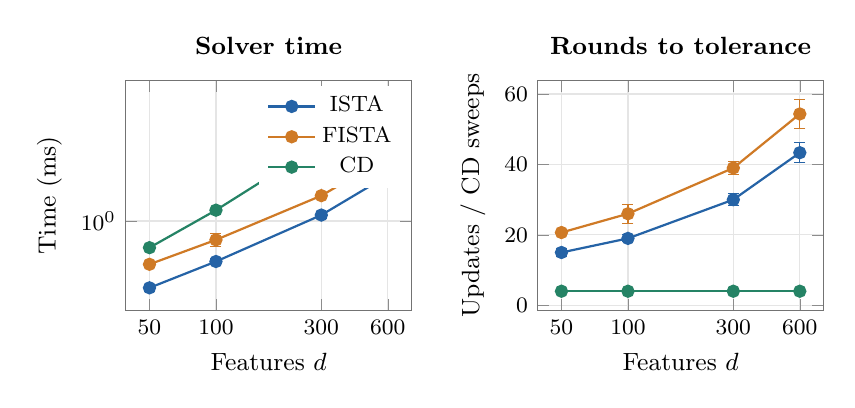
\begin{tikzpicture}
\begin{groupplot}[group style={group size=2 by 1,horizontal sep=1.6cm},width=.43\linewidth,height=4.5cm,xmode=log,xtick={50,100,300,600},xticklabels={50,100,300,600},minor tick num=0,xlabel={Features $d$},grid=major]
\nextgroupplot[title={Solver time},ylabel={Time (ms)},ymode=log]
\addplot[lassoblue,thick,mark=*,error bars/.cd,y dir=both,y explicit] coordinates {(50,0.34129167) +- (0,0.01811425) (100,0.52109767) +- (0,0.026096299) (300,1.099736) +- (0,0.059208238) (600,2.0782083) +- (0,0.12413283)};
\addlegendentry{ISTA}
\addplot[lassoorange,thick,mark=*,error bars/.cd,y dir=both,y explicit] coordinates {(50,0.49827767) +- (0,0.0034995812) (100,0.73816667) +- (0,0.075594418) (300,1.5023053) +- (0,0.039706889) (600,2.7954163) +- (0,0.19431844)};
\addlegendentry{FISTA}
\addplot[lassogreen,thick,mark=*,error bars/.cd,y dir=both,y explicit] coordinates {(50,0.650972) +- (0,0.015342767) (100,1.1894167) +- (0,0.010011867) (300,3.4560277) +- (0,0.023972544) (600,6.972194) +- (0,0.053164411)};
\addlegendentry{CD}
\nextgroupplot[title={Rounds to tolerance},ylabel={Updates / CD sweeps}]
\addplot[lassoblue,thick,mark=*,error bars/.cd,y dir=both,y explicit] coordinates {(50,15) +- (0,1) (100,19) +- (0,1) (300,30) +- (0,1.7320508) (600,43.333333) +- (0,2.8867513)};
\addplot[lassoorange,thick,mark=*,error bars/.cd,y dir=both,y explicit] coordinates {(50,20.666667) +- (0,0.57735027) (100,26) +- (0,2.6457513) (300,39) +- (0,1.7320508) (600,54.333333) +- (0,4.0414519)};
\addplot[lassogreen,thick,mark=*,error bars/.cd,y dir=both,y explicit] coordinates {(50,4) +- (0,0) (100,4) +- (0,0) (300,4) +- (0,0) (600,4) +- (0,0)};
\end{groupplot}
\end{tikzpicture}
\caption{Feature-count study with 800 training observations. Means and sample SD across three instance medians; five timings per instance. Shared spectral setup is excluded.}\label{fig:dimension}\end{minipage}\end{center}

\subsection{Coefficient paths and fitting error}
The original four-penalty study is extended to 34 pre-specified values between $0.01\lambda_{\max}$ and $\lambda_{\max}$ on synthetic seed 0 and the fixed Diabetes split. CD starts from zero for each fit and reaches the same tolerance. Figure~\ref{fig:paths} records the coefficients as well as training and test MSE, without selecting a penalty from test scores.

The synthetic paths show retained coefficients approaching zero as the penalty strengthens; weaker penalties also admit small coefficients on inactive variables. On Diabetes, the five highlighted paths are the predictors selected at the main ratio 0.1, not a known true support. Their magnitudes need not all shrink monotonically: s3 first moves farther below zero before returning toward zero. Unlike the orthogonal formula, correlated predictors are fitted jointly, and the penalty changes their allocation of the shared signal.

Large penalties increase fitting error sharply on both fixed splits. Training MSE can exceed test MSE on a particular split; these curves are neither uncertainty estimates nor a generalization bound. A validation procedure would be needed to select a penalty for prediction. The paths explain how the model changes, while the timing studies compare how different algorithms solve a fixed model.

\begin{center}\begin{minipage}{\linewidth}\captionsetup{type=figure}\centering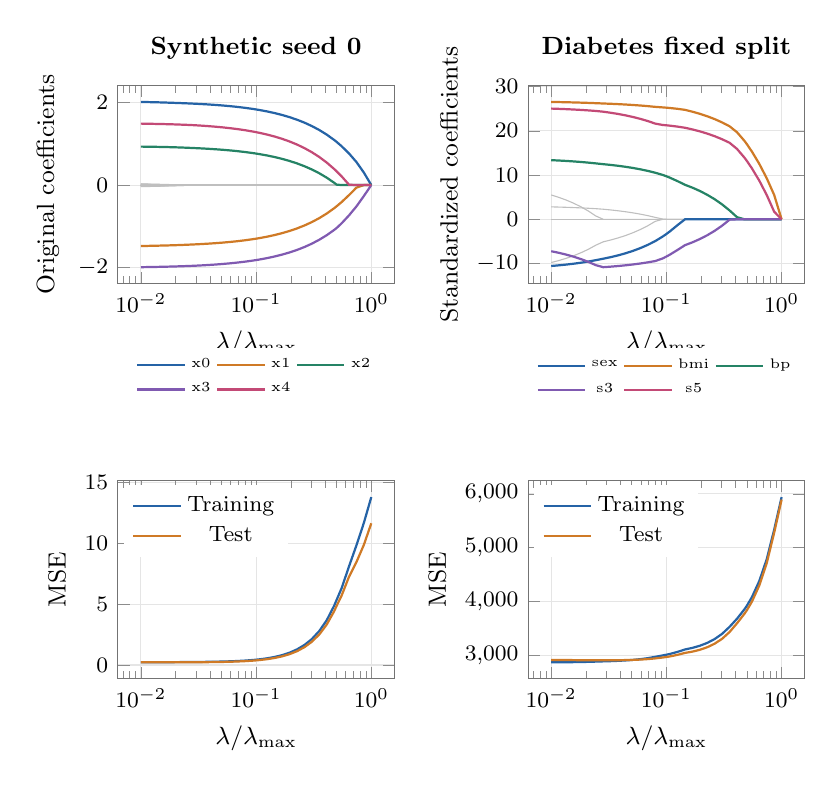
\begin{tikzpicture}
\begin{groupplot}[group style={group size=2 by 2,horizontal sep=1.7cm,vertical sep=2.5cm},width=.42\linewidth,height=4.1cm,xmode=log,xlabel={$\lambda/\lambda_{\max}$},grid=major]
\nextgroupplot[title={Synthetic seed 0},ylabel={Original coefficients},legend style={at={(.5,-.32)},anchor=north,legend columns=3,font=\tiny}]
\addplot[black!25,thin,forget plot] coordinates {(0.01,0.025091556) (0.011601553,0.020310535) (0.013459603,0.015070051) (0.01561523,0.009060596) (0.018116092,0.0020638338) (0.02101748,0) (0.024383541,0) (0.028288694,0) (0.032819279,0) (0.03807546,0) (0.044173447,0) (0.051248059,0) (0.059455707,0) (0.068977854,0) (0.080025023,0) (0.092841454,0) (0.1,0) (0.10771051,0) (0.12496091,0) (0.14497407,0) (0.16819243,0) (0.19512934,0) (0.22638034,0) (0.26263635,0) (0.30469896,0) (0.35349811,0) (0.41011271,0) (0.47579443,-0) (0.5,-0) (0.55199543,-0) (0.64040043,-0) (0.74296395,-0) (0.86195357,-0) (1,0)};
\addplot[black!25,thin,forget plot] coordinates {(0.01,-0) (0.011601553,-0) (0.013459603,-0) (0.01561523,-0) (0.018116092,-0) (0.02101748,-0) (0.024383541,-0) (0.028288694,-0) (0.032819279,-0) (0.03807546,-0) (0.044173447,-0) (0.051248059,0) (0.059455707,0) (0.068977854,0) (0.080025023,0) (0.092841454,0) (0.1,0) (0.10771051,0) (0.12496091,0) (0.14497407,0) (0.16819243,0) (0.19512934,0) (0.22638034,0) (0.26263635,0) (0.30469896,0) (0.35349811,0) (0.41011271,0) (0.47579443,0) (0.5,0) (0.55199543,0) (0.64040043,0) (0.74296395,0) (0.86195357,0) (1,0)};
\addplot[black!25,thin,forget plot] coordinates {(0.01,0.016154619) (0.011601553,0.013251933) (0.013459603,0.0097252544) (0.01561523,0.0056263773) (0.018116092,0.00068083543) (0.02101748,0) (0.024383541,0) (0.028288694,0) (0.032819279,0) (0.03807546,0) (0.044173447,0) (0.051248059,0) (0.059455707,0) (0.068977854,0) (0.080025023,0) (0.092841454,0) (0.1,0) (0.10771051,0) (0.12496091,0) (0.14497407,0) (0.16819243,0) (0.19512934,0) (0.22638034,0) (0.26263635,0) (0.30469896,0) (0.35349811,0) (0.41011271,0) (0.47579443,0) (0.5,0) (0.55199543,0) (0.64040043,-0) (0.74296395,-0) (0.86195357,-0) (1,0)};
\addplot[black!25,thin,forget plot] coordinates {(0.01,-0) (0.011601553,-0) (0.013459603,-0) (0.01561523,-0) (0.018116092,-0) (0.02101748,-0) (0.024383541,-0) (0.028288694,-0) (0.032819279,-0) (0.03807546,-0) (0.044173447,-0) (0.051248059,-0) (0.059455707,0) (0.068977854,0) (0.080025023,0) (0.092841454,0) (0.1,0) (0.10771051,0) (0.12496091,0) (0.14497407,0) (0.16819243,0) (0.19512934,0) (0.22638034,0) (0.26263635,0) (0.30469896,0) (0.35349811,0) (0.41011271,0) (0.47579443,0) (0.5,0) (0.55199543,0) (0.64040043,0) (0.74296395,0) (0.86195357,0) (1,0)};
\addplot[black!25,thin,forget plot] coordinates {(0.01,0) (0.011601553,0) (0.013459603,0) (0.01561523,0) (0.018116092,0) (0.02101748,0) (0.024383541,0) (0.028288694,-0) (0.032819279,-0) (0.03807546,-0) (0.044173447,-0) (0.051248059,-0) (0.059455707,-0) (0.068977854,-0) (0.080025023,-0) (0.092841454,-0) (0.1,-0) (0.10771051,-0) (0.12496091,-0) (0.14497407,-0) (0.16819243,-0) (0.19512934,-0) (0.22638034,-0) (0.26263635,-0) (0.30469896,-0) (0.35349811,-0) (0.41011271,-0) (0.47579443,-0) (0.5,-0) (0.55199543,-0) (0.64040043,-0) (0.74296395,-0) (0.86195357,-0) (1,0)};
\addplot[black!25,thin,forget plot] coordinates {(0.01,0.027776788) (0.011601553,0.02426443) (0.013459603,0.020584247) (0.01561523,0.016387664) (0.018116092,0.011257426) (0.02101748,0.00561384) (0.024383541,0) (0.028288694,0) (0.032819279,0) (0.03807546,0) (0.044173447,0) (0.051248059,0) (0.059455707,0) (0.068977854,0) (0.080025023,0) (0.092841454,0) (0.1,0) (0.10771051,0) (0.12496091,0) (0.14497407,0) (0.16819243,0) (0.19512934,0) (0.22638034,0) (0.26263635,0) (0.30469896,0) (0.35349811,0) (0.41011271,0) (0.47579443,0) (0.5,0) (0.55199543,0) (0.64040043,0) (0.74296395,0) (0.86195357,0) (1,0)};
\addplot[black!25,thin,forget plot] coordinates {(0.01,-0.00096840526) (0.011601553,-0) (0.013459603,-0) (0.01561523,-0) (0.018116092,-0) (0.02101748,-0) (0.024383541,-0) (0.028288694,-0) (0.032819279,-0) (0.03807546,-0) (0.044173447,-0) (0.051248059,-0) (0.059455707,-0) (0.068977854,-0) (0.080025023,-0) (0.092841454,-0) (0.1,-0) (0.10771051,-0) (0.12496091,-0) (0.14497407,-0) (0.16819243,-0) (0.19512934,-0) (0.22638034,-0) (0.26263635,-0) (0.30469896,-0) (0.35349811,-0) (0.41011271,-0) (0.47579443,-0) (0.5,-0) (0.55199543,-0) (0.64040043,-0) (0.74296395,-0) (0.86195357,-0) (1,0)};
\addplot[black!25,thin,forget plot] coordinates {(0.01,-0) (0.011601553,-0) (0.013459603,-0) (0.01561523,-0) (0.018116092,-0) (0.02101748,-0) (0.024383541,-0) (0.028288694,-0) (0.032819279,-0) (0.03807546,-0) (0.044173447,-0) (0.051248059,-0) (0.059455707,-0) (0.068977854,-0) (0.080025023,-0) (0.092841454,-0) (0.1,-0) (0.10771051,-0) (0.12496091,-0) (0.14497407,-0) (0.16819243,-0) (0.19512934,-0) (0.22638034,-0) (0.26263635,-0) (0.30469896,-0) (0.35349811,0) (0.41011271,0) (0.47579443,0) (0.5,0) (0.55199543,0) (0.64040043,0) (0.74296395,0) (0.86195357,0) (1,0)};
\addplot[black!25,thin,forget plot] coordinates {(0.01,-0.031608315) (0.011601553,-0.028872756) (0.013459603,-0.025850521) (0.01561523,-0.022353758) (0.018116092,-0.018249557) (0.02101748,-0.013555422) (0.024383541,-0.0081326501) (0.028288694,-0.0018136594) (0.032819279,-0) (0.03807546,-0) (0.044173447,-0) (0.051248059,-0) (0.059455707,-0) (0.068977854,-0) (0.080025023,-0) (0.092841454,-0) (0.1,-0) (0.10771051,-0) (0.12496091,-0) (0.14497407,-0) (0.16819243,-0) (0.19512934,-0) (0.22638034,-0) (0.26263635,-0) (0.30469896,-0) (0.35349811,-0) (0.41011271,-0) (0.47579443,-0) (0.5,-0) (0.55199543,-0) (0.64040043,-0) (0.74296395,-0) (0.86195357,-0) (1,0)};
\addplot[black!25,thin,forget plot] coordinates {(0.01,0) (0.011601553,0) (0.013459603,0) (0.01561523,0) (0.018116092,0) (0.02101748,0) (0.024383541,0) (0.028288694,0) (0.032819279,0) (0.03807546,0) (0.044173447,0) (0.051248059,0) (0.059455707,0) (0.068977854,0) (0.080025023,0) (0.092841454,0) (0.1,0) (0.10771051,0) (0.12496091,0) (0.14497407,0) (0.16819243,0) (0.19512934,0) (0.22638034,0) (0.26263635,0) (0.30469896,0) (0.35349811,0) (0.41011271,0) (0.47579443,0) (0.5,0) (0.55199543,0) (0.64040043,0) (0.74296395,0) (0.86195357,0) (1,0)};
\addplot[black!25,thin,forget plot] coordinates {(0.01,0.015108675) (0.011601553,0.012158496) (0.013459603,0.00866049) (0.01561523,0.004490107) (0.018116092,5.0781328e-05) (0.02101748,0) (0.024383541,0) (0.028288694,0) (0.032819279,0) (0.03807546,0) (0.044173447,0) (0.051248059,0) (0.059455707,0) (0.068977854,0) (0.080025023,0) (0.092841454,0) (0.1,0) (0.10771051,0) (0.12496091,0) (0.14497407,0) (0.16819243,0) (0.19512934,0) (0.22638034,0) (0.26263635,0) (0.30469896,0) (0.35349811,0) (0.41011271,0) (0.47579443,0) (0.5,0) (0.55199543,0) (0.64040043,0) (0.74296395,0) (0.86195357,0) (1,0)};
\addplot[black!25,thin,forget plot] coordinates {(0.01,-0.014969888) (0.011601553,-0.013105361) (0.013459603,-0.010395416) (0.01561523,-0.0070183453) (0.018116092,-0.0026910598) (0.02101748,-0) (0.024383541,-0) (0.028288694,-0) (0.032819279,-0) (0.03807546,-0) (0.044173447,-0) (0.051248059,-0) (0.059455707,-0) (0.068977854,-0) (0.080025023,-0) (0.092841454,-0) (0.1,-0) (0.10771051,-0) (0.12496091,-0) (0.14497407,-0) (0.16819243,-0) (0.19512934,-0) (0.22638034,-0) (0.26263635,-0) (0.30469896,-0) (0.35349811,-0) (0.41011271,0) (0.47579443,0) (0.5,0) (0.55199543,0) (0.64040043,0) (0.74296395,0) (0.86195357,0) (1,0)};
\addplot[black!25,thin,forget plot] coordinates {(0.01,0) (0.011601553,-0) (0.013459603,-0) (0.01561523,-0) (0.018116092,-0) (0.02101748,-0) (0.024383541,-0) (0.028288694,-0) (0.032819279,-0) (0.03807546,-0) (0.044173447,-0) (0.051248059,-0) (0.059455707,-0) (0.068977854,-0) (0.080025023,-0) (0.092841454,-0) (0.1,-0) (0.10771051,-0) (0.12496091,-0) (0.14497407,-0) (0.16819243,-0) (0.19512934,-0) (0.22638034,-0) (0.26263635,-0) (0.30469896,-0) (0.35349811,-0) (0.41011271,-0) (0.47579443,-0) (0.5,-0) (0.55199543,-0) (0.64040043,-0) (0.74296395,-0) (0.86195357,-0) (1,0)};
\addplot[black!25,thin,forget plot] coordinates {(0.01,0) (0.011601553,0) (0.013459603,0) (0.01561523,0) (0.018116092,0) (0.02101748,0) (0.024383541,0) (0.028288694,0) (0.032819279,0) (0.03807546,0) (0.044173447,0) (0.051248059,0) (0.059455707,-0) (0.068977854,-0) (0.080025023,-0) (0.092841454,-0) (0.1,-0) (0.10771051,-0) (0.12496091,-0) (0.14497407,-0) (0.16819243,-0) (0.19512934,-0) (0.22638034,-0) (0.26263635,-0) (0.30469896,-0) (0.35349811,-0) (0.41011271,-0) (0.47579443,-0) (0.5,-0) (0.55199543,-0) (0.64040043,-0) (0.74296395,-0) (0.86195357,-0) (1,0)};
\addplot[black!25,thin,forget plot] coordinates {(0.01,0) (0.011601553,0) (0.013459603,0) (0.01561523,0) (0.018116092,0) (0.02101748,0) (0.024383541,0) (0.028288694,0) (0.032819279,0) (0.03807546,0) (0.044173447,0) (0.051248059,-0) (0.059455707,-0) (0.068977854,-0) (0.080025023,-0) (0.092841454,-0) (0.1,-0) (0.10771051,-0) (0.12496091,-0) (0.14497407,-0) (0.16819243,-0) (0.19512934,-0) (0.22638034,-0) (0.26263635,-0) (0.30469896,-0) (0.35349811,-0) (0.41011271,-0) (0.47579443,-0) (0.5,-0) (0.55199543,-0) (0.64040043,-0) (0.74296395,-0) (0.86195357,-0) (1,0)};
\addplot[black!25,thin,forget plot] coordinates {(0.01,0) (0.011601553,0) (0.013459603,0) (0.01561523,0) (0.018116092,0) (0.02101748,0) (0.024383541,0) (0.028288694,0) (0.032819279,0) (0.03807546,0) (0.044173447,0) (0.051248059,0) (0.059455707,0) (0.068977854,0) (0.080025023,0) (0.092841454,0) (0.1,0) (0.10771051,0) (0.12496091,0) (0.14497407,0) (0.16819243,0) (0.19512934,0) (0.22638034,0) (0.26263635,0) (0.30469896,0) (0.35349811,0) (0.41011271,0) (0.47579443,0) (0.5,0) (0.55199543,0) (0.64040043,0) (0.74296395,0) (0.86195357,0) (1,0)};
\addplot[black!25,thin,forget plot] coordinates {(0.01,-0.038261387) (0.011601553,-0.034804818) (0.013459603,-0.030622538) (0.01561523,-0.025684024) (0.018116092,-0.020082427) (0.02101748,-0.014412227) (0.024383541,-0.0082528377) (0.028288694,-0.00062650239) (0.032819279,-0) (0.03807546,-0) (0.044173447,-0) (0.051248059,-0) (0.059455707,-0) (0.068977854,-0) (0.080025023,-0) (0.092841454,-0) (0.1,-0) (0.10771051,-0) (0.12496091,-0) (0.14497407,-0) (0.16819243,-0) (0.19512934,-0) (0.22638034,-0) (0.26263635,-0) (0.30469896,-0) (0.35349811,-0) (0.41011271,-0) (0.47579443,-0) (0.5,-0) (0.55199543,-0) (0.64040043,-0) (0.74296395,0) (0.86195357,0) (1,0)};
\addplot[black!25,thin,forget plot] coordinates {(0.01,0) (0.011601553,0) (0.013459603,0) (0.01561523,0) (0.018116092,0) (0.02101748,0) (0.024383541,0) (0.028288694,0) (0.032819279,0) (0.03807546,0) (0.044173447,0) (0.051248059,0) (0.059455707,0) (0.068977854,-0) (0.080025023,-0) (0.092841454,-0) (0.1,-0) (0.10771051,-0) (0.12496091,-0) (0.14497407,-0) (0.16819243,-0) (0.19512934,-0) (0.22638034,-0) (0.26263635,-0) (0.30469896,-0) (0.35349811,-0) (0.41011271,-0) (0.47579443,-0) (0.5,-0) (0.55199543,-0) (0.64040043,-0) (0.74296395,-0) (0.86195357,-0) (1,0)};
\addplot[black!25,thin,forget plot] coordinates {(0.01,-0) (0.011601553,-0) (0.013459603,-0) (0.01561523,-0) (0.018116092,-0) (0.02101748,-0) (0.024383541,-0) (0.028288694,0) (0.032819279,0) (0.03807546,0) (0.044173447,0) (0.051248059,0) (0.059455707,0) (0.068977854,0) (0.080025023,0) (0.092841454,0) (0.1,0) (0.10771051,0) (0.12496091,0) (0.14497407,0) (0.16819243,0) (0.19512934,0) (0.22638034,0) (0.26263635,0) (0.30469896,0) (0.35349811,0) (0.41011271,0) (0.47579443,0) (0.5,0) (0.55199543,0) (0.64040043,0) (0.74296395,0) (0.86195357,0) (1,0)};
\addplot[black!25,thin,forget plot] coordinates {(0.01,-0) (0.011601553,-0) (0.013459603,-0) (0.01561523,-0) (0.018116092,-0) (0.02101748,-0) (0.024383541,-0) (0.028288694,-0) (0.032819279,-0) (0.03807546,-0) (0.044173447,0) (0.051248059,0) (0.059455707,0) (0.068977854,0) (0.080025023,0) (0.092841454,0) (0.1,0) (0.10771051,0) (0.12496091,0) (0.14497407,0) (0.16819243,0) (0.19512934,0) (0.22638034,0) (0.26263635,0) (0.30469896,0) (0.35349811,0) (0.41011271,0) (0.47579443,0) (0.5,0) (0.55199543,0) (0.64040043,0) (0.74296395,0) (0.86195357,0) (1,0)};
\addplot[black!25,thin,forget plot] coordinates {(0.01,-0.01604251) (0.011601553,-0.01313441) (0.013459603,-0.0095849799) (0.01561523,-0.0054262279) (0.018116092,-0.00072179236) (0.02101748,-0) (0.024383541,-0) (0.028288694,-0) (0.032819279,-0) (0.03807546,-0) (0.044173447,-0) (0.051248059,-0) (0.059455707,-0) (0.068977854,-0) (0.080025023,-0) (0.092841454,-0) (0.1,-0) (0.10771051,-0) (0.12496091,-0) (0.14497407,-0) (0.16819243,-0) (0.19512934,-0) (0.22638034,-0) (0.26263635,-0) (0.30469896,-0) (0.35349811,-0) (0.41011271,-0) (0.47579443,-0) (0.5,-0) (0.55199543,-0) (0.64040043,-0) (0.74296395,-0) (0.86195357,-0) (1,0)};
\addplot[black!25,thin,forget plot] coordinates {(0.01,-0.001727377) (0.011601553,-0) (0.013459603,-0) (0.01561523,-0) (0.018116092,-0) (0.02101748,-0) (0.024383541,-0) (0.028288694,-0) (0.032819279,-0) (0.03807546,-0) (0.044173447,-0) (0.051248059,-0) (0.059455707,-0) (0.068977854,-0) (0.080025023,-0) (0.092841454,-0) (0.1,-0) (0.10771051,-0) (0.12496091,-0) (0.14497407,0) (0.16819243,0) (0.19512934,0) (0.22638034,0) (0.26263635,0) (0.30469896,0) (0.35349811,0) (0.41011271,0) (0.47579443,0) (0.5,0) (0.55199543,0) (0.64040043,0) (0.74296395,0) (0.86195357,0) (1,0)};
\addplot[black!25,thin,forget plot] coordinates {(0.01,-0) (0.011601553,-0) (0.013459603,-0) (0.01561523,-0) (0.018116092,-0) (0.02101748,-0) (0.024383541,-0) (0.028288694,-0) (0.032819279,-0) (0.03807546,-0) (0.044173447,-0) (0.051248059,-0) (0.059455707,-0) (0.068977854,-0) (0.080025023,-0) (0.092841454,-0) (0.1,-0) (0.10771051,-0) (0.12496091,-0) (0.14497407,-0) (0.16819243,-0) (0.19512934,-0) (0.22638034,-0) (0.26263635,-0) (0.30469896,-0) (0.35349811,-0) (0.41011271,-0) (0.47579443,-0) (0.5,-0) (0.55199543,-0) (0.64040043,-0) (0.74296395,-0) (0.86195357,-0) (1,0)};
\addplot[black!25,thin,forget plot] coordinates {(0.01,-0) (0.011601553,-0) (0.013459603,-0) (0.01561523,-0) (0.018116092,-0) (0.02101748,-0) (0.024383541,-0) (0.028288694,-0) (0.032819279,-0) (0.03807546,-0) (0.044173447,-0) (0.051248059,-0) (0.059455707,-0) (0.068977854,-0) (0.080025023,-0) (0.092841454,-0) (0.1,-0) (0.10771051,-0) (0.12496091,-0) (0.14497407,-0) (0.16819243,-0) (0.19512934,-0) (0.22638034,-0) (0.26263635,-0) (0.30469896,-0) (0.35349811,-0) (0.41011271,-0) (0.47579443,-0) (0.5,-0) (0.55199543,-0) (0.64040043,-0) (0.74296395,-0) (0.86195357,-0) (1,0)};
\addplot[black!25,thin,forget plot] coordinates {(0.01,-0) (0.011601553,-0) (0.013459603,-0) (0.01561523,-0) (0.018116092,-0) (0.02101748,-0) (0.024383541,-0) (0.028288694,-0) (0.032819279,-0) (0.03807546,-0) (0.044173447,-0) (0.051248059,-0) (0.059455707,-0) (0.068977854,-0) (0.080025023,-0) (0.092841454,-0) (0.1,-0) (0.10771051,-0) (0.12496091,-0) (0.14497407,-0) (0.16819243,-0) (0.19512934,-0) (0.22638034,-0) (0.26263635,-0) (0.30469896,-0) (0.35349811,-0) (0.41011271,-0) (0.47579443,-0) (0.5,-0) (0.55199543,-0) (0.64040043,-0) (0.74296395,-0) (0.86195357,-0) (1,0)};
\addplot[black!25,thin,forget plot] coordinates {(0.01,-0) (0.011601553,-0) (0.013459603,-0) (0.01561523,-0) (0.018116092,-0) (0.02101748,-0) (0.024383541,-0) (0.028288694,-0) (0.032819279,-0) (0.03807546,-0) (0.044173447,-0) (0.051248059,-0) (0.059455707,-0) (0.068977854,-0) (0.080025023,-0) (0.092841454,-0) (0.1,-0) (0.10771051,-0) (0.12496091,-0) (0.14497407,-0) (0.16819243,-0) (0.19512934,-0) (0.22638034,-0) (0.26263635,-0) (0.30469896,-0) (0.35349811,-0) (0.41011271,-0) (0.47579443,-0) (0.5,-0) (0.55199543,-0) (0.64040043,-0) (0.74296395,-0) (0.86195357,-0) (1,0)};
\addplot[black!25,thin,forget plot] coordinates {(0.01,0.0089255442) (0.011601553,0.0064942866) (0.013459603,0.0032626231) (0.01561523,0) (0.018116092,0) (0.02101748,0) (0.024383541,0) (0.028288694,0) (0.032819279,0) (0.03807546,0) (0.044173447,0) (0.051248059,0) (0.059455707,0) (0.068977854,0) (0.080025023,0) (0.092841454,0) (0.1,0) (0.10771051,0) (0.12496091,0) (0.14497407,0) (0.16819243,0) (0.19512934,0) (0.22638034,0) (0.26263635,0) (0.30469896,0) (0.35349811,0) (0.41011271,0) (0.47579443,0) (0.5,0) (0.55199543,0) (0.64040043,0) (0.74296395,0) (0.86195357,0) (1,0)};
\addplot[black!25,thin,forget plot] coordinates {(0.01,0) (0.011601553,0) (0.013459603,0) (0.01561523,0) (0.018116092,0) (0.02101748,0) (0.024383541,0) (0.028288694,0) (0.032819279,0) (0.03807546,0) (0.044173447,0) (0.051248059,0) (0.059455707,0) (0.068977854,0) (0.080025023,0) (0.092841454,0) (0.1,0) (0.10771051,0) (0.12496091,0) (0.14497407,-0) (0.16819243,-0) (0.19512934,-0) (0.22638034,-0) (0.26263635,-0) (0.30469896,-0) (0.35349811,-0) (0.41011271,-0) (0.47579443,-0) (0.5,-0) (0.55199543,-0) (0.64040043,-0) (0.74296395,-0) (0.86195357,-0) (1,0)};
\addplot[black!25,thin,forget plot] coordinates {(0.01,-0) (0.011601553,-0) (0.013459603,-0) (0.01561523,-0) (0.018116092,-0) (0.02101748,-0) (0.024383541,-0) (0.028288694,-0) (0.032819279,0) (0.03807546,0) (0.044173447,0) (0.051248059,0) (0.059455707,0) (0.068977854,0) (0.080025023,0) (0.092841454,0) (0.1,0) (0.10771051,0) (0.12496091,0) (0.14497407,0) (0.16819243,0) (0.19512934,0) (0.22638034,0) (0.26263635,0) (0.30469896,0) (0.35349811,0) (0.41011271,0) (0.47579443,0) (0.5,0) (0.55199543,0) (0.64040043,0) (0.74296395,0) (0.86195357,0) (1,0)};
\addplot[black!25,thin,forget plot] coordinates {(0.01,0) (0.011601553,0) (0.013459603,0) (0.01561523,0) (0.018116092,0) (0.02101748,0) (0.024383541,0) (0.028288694,0) (0.032819279,0) (0.03807546,0) (0.044173447,0) (0.051248059,0) (0.059455707,0) (0.068977854,0) (0.080025023,0) (0.092841454,0) (0.1,0) (0.10771051,0) (0.12496091,-0) (0.14497407,-0) (0.16819243,-0) (0.19512934,-0) (0.22638034,-0) (0.26263635,-0) (0.30469896,-0) (0.35349811,-0) (0.41011271,-0) (0.47579443,-0) (0.5,-0) (0.55199543,-0) (0.64040043,-0) (0.74296395,-0) (0.86195357,-0) (1,0)};
\addplot[black!25,thin,forget plot] coordinates {(0.01,0) (0.011601553,0) (0.013459603,0) (0.01561523,0) (0.018116092,0) (0.02101748,0) (0.024383541,0) (0.028288694,0) (0.032819279,-0) (0.03807546,-0) (0.044173447,-0) (0.051248059,-0) (0.059455707,-0) (0.068977854,-0) (0.080025023,-0) (0.092841454,-0) (0.1,-0) (0.10771051,-0) (0.12496091,-0) (0.14497407,-0) (0.16819243,-0) (0.19512934,-0) (0.22638034,-0) (0.26263635,-0) (0.30469896,-0) (0.35349811,-0) (0.41011271,-0) (0.47579443,-0) (0.5,-0) (0.55199543,-0) (0.64040043,-0) (0.74296395,-0) (0.86195357,-0) (1,0)};
\addplot[black!25,thin,forget plot] coordinates {(0.01,-0) (0.011601553,-0) (0.013459603,-0) (0.01561523,-0) (0.018116092,-0) (0.02101748,-0) (0.024383541,-0) (0.028288694,0) (0.032819279,0) (0.03807546,0) (0.044173447,0) (0.051248059,0) (0.059455707,0) (0.068977854,0) (0.080025023,0) (0.092841454,0) (0.1,0) (0.10771051,0) (0.12496091,0) (0.14497407,0) (0.16819243,0) (0.19512934,0) (0.22638034,0) (0.26263635,0) (0.30469896,0) (0.35349811,0) (0.41011271,0) (0.47579443,0) (0.5,0) (0.55199543,0) (0.64040043,0) (0.74296395,0) (0.86195357,0) (1,0)};
\addplot[black!25,thin,forget plot] coordinates {(0.01,-0.0045411436) (0.011601553,-0.0013691103) (0.013459603,-0) (0.01561523,-0) (0.018116092,-0) (0.02101748,-0) (0.024383541,-0) (0.028288694,-0) (0.032819279,-0) (0.03807546,-0) (0.044173447,-0) (0.051248059,-0) (0.059455707,-0) (0.068977854,-0) (0.080025023,-0) (0.092841454,-0) (0.1,-0) (0.10771051,-0) (0.12496091,-0) (0.14497407,-0) (0.16819243,-0) (0.19512934,-0) (0.22638034,-0) (0.26263635,-0) (0.30469896,-0) (0.35349811,-0) (0.41011271,-0) (0.47579443,-0) (0.5,-0) (0.55199543,-0) (0.64040043,-0) (0.74296395,0) (0.86195357,0) (1,0)};
\addplot[black!25,thin,forget plot] coordinates {(0.01,-0) (0.011601553,-0) (0.013459603,-0) (0.01561523,-0) (0.018116092,-0) (0.02101748,-0) (0.024383541,-0) (0.028288694,-0) (0.032819279,-0) (0.03807546,-0) (0.044173447,-0) (0.051248059,-0) (0.059455707,-0) (0.068977854,-0) (0.080025023,-0) (0.092841454,-0) (0.1,-0) (0.10771051,-0) (0.12496091,-0) (0.14497407,0) (0.16819243,0) (0.19512934,0) (0.22638034,0) (0.26263635,0) (0.30469896,0) (0.35349811,0) (0.41011271,0) (0.47579443,0) (0.5,0) (0.55199543,0) (0.64040043,0) (0.74296395,0) (0.86195357,0) (1,0)};
\addplot[black!25,thin,forget plot] coordinates {(0.01,0) (0.011601553,0) (0.013459603,0) (0.01561523,0) (0.018116092,0) (0.02101748,0) (0.024383541,0) (0.028288694,0) (0.032819279,0) (0.03807546,0) (0.044173447,0) (0.051248059,0) (0.059455707,0) (0.068977854,0) (0.080025023,0) (0.092841454,0) (0.1,0) (0.10771051,0) (0.12496091,0) (0.14497407,0) (0.16819243,0) (0.19512934,0) (0.22638034,0) (0.26263635,0) (0.30469896,0) (0.35349811,0) (0.41011271,0) (0.47579443,0) (0.5,0) (0.55199543,0) (0.64040043,0) (0.74296395,0) (0.86195357,0) (1,0)};
\addplot[black!25,thin,forget plot] coordinates {(0.01,-0.017052871) (0.011601553,-0.014028314) (0.013459603,-0.010619958) (0.01561523,-0.0067509572) (0.018116092,-0.0020373016) (0.02101748,-0) (0.024383541,-0) (0.028288694,-0) (0.032819279,-0) (0.03807546,-0) (0.044173447,-0) (0.051248059,-0) (0.059455707,-0) (0.068977854,-0) (0.080025023,-0) (0.092841454,-0) (0.1,-0) (0.10771051,-0) (0.12496091,-0) (0.14497407,-0) (0.16819243,-0) (0.19512934,-0) (0.22638034,-0) (0.26263635,-0) (0.30469896,-0) (0.35349811,-0) (0.41011271,-0) (0.47579443,0) (0.5,0) (0.55199543,0) (0.64040043,0) (0.74296395,-0) (0.86195357,-0) (1,0)};
\addplot[black!25,thin,forget plot] coordinates {(0.01,-0.0023289071) (0.011601553,-0) (0.013459603,-0) (0.01561523,-0) (0.018116092,-0) (0.02101748,-0) (0.024383541,-0) (0.028288694,-0) (0.032819279,-0) (0.03807546,-0) (0.044173447,-0) (0.051248059,-0) (0.059455707,-0) (0.068977854,-0) (0.080025023,0) (0.092841454,0) (0.1,0) (0.10771051,0) (0.12496091,0) (0.14497407,0) (0.16819243,0) (0.19512934,0) (0.22638034,0) (0.26263635,0) (0.30469896,0) (0.35349811,0) (0.41011271,0) (0.47579443,0) (0.5,0) (0.55199543,0) (0.64040043,0) (0.74296395,0) (0.86195357,0) (1,0)};
\addplot[black!25,thin,forget plot] coordinates {(0.01,0) (0.011601553,0) (0.013459603,0) (0.01561523,0) (0.018116092,0) (0.02101748,-0) (0.024383541,-0) (0.028288694,-0) (0.032819279,-0) (0.03807546,-0) (0.044173447,-0) (0.051248059,-0) (0.059455707,-0) (0.068977854,-0) (0.080025023,-0) (0.092841454,-0) (0.1,-0) (0.10771051,-0) (0.12496091,-0) (0.14497407,-0) (0.16819243,-0) (0.19512934,-0) (0.22638034,-0) (0.26263635,-0) (0.30469896,-0) (0.35349811,-0) (0.41011271,-0) (0.47579443,-0) (0.5,-0) (0.55199543,-0) (0.64040043,-0) (0.74296395,-0) (0.86195357,-0) (1,0)};
\addplot[black!25,thin,forget plot] coordinates {(0.01,0) (0.011601553,0) (0.013459603,0) (0.01561523,0) (0.018116092,0) (0.02101748,0) (0.024383541,0) (0.028288694,0) (0.032819279,0) (0.03807546,0) (0.044173447,0) (0.051248059,0) (0.059455707,0) (0.068977854,0) (0.080025023,0) (0.092841454,0) (0.1,0) (0.10771051,0) (0.12496091,-0) (0.14497407,-0) (0.16819243,-0) (0.19512934,-0) (0.22638034,-0) (0.26263635,-0) (0.30469896,-0) (0.35349811,-0) (0.41011271,-0) (0.47579443,-0) (0.5,-0) (0.55199543,-0) (0.64040043,-0) (0.74296395,-0) (0.86195357,-0) (1,0)};
\addplot[black!25,thin,forget plot] coordinates {(0.01,0) (0.011601553,0) (0.013459603,0) (0.01561523,0) (0.018116092,0) (0.02101748,0) (0.024383541,0) (0.028288694,0) (0.032819279,0) (0.03807546,0) (0.044173447,0) (0.051248059,0) (0.059455707,0) (0.068977854,0) (0.080025023,0) (0.092841454,0) (0.1,0) (0.10771051,0) (0.12496091,0) (0.14497407,0) (0.16819243,0) (0.19512934,0) (0.22638034,0) (0.26263635,0) (0.30469896,0) (0.35349811,0) (0.41011271,0) (0.47579443,0) (0.5,0) (0.55199543,0) (0.64040043,0) (0.74296395,0) (0.86195357,0) (1,0)};
\addplot[black!25,thin,forget plot] coordinates {(0.01,-0) (0.011601553,-0) (0.013459603,-0) (0.01561523,-0) (0.018116092,-0) (0.02101748,-0) (0.024383541,-0) (0.028288694,-0) (0.032819279,-0) (0.03807546,-0) (0.044173447,-0) (0.051248059,-0) (0.059455707,-0) (0.068977854,-0) (0.080025023,-0) (0.092841454,-0) (0.1,-0) (0.10771051,-0) (0.12496091,-0) (0.14497407,-0) (0.16819243,-0) (0.19512934,-0) (0.22638034,-0) (0.26263635,-0) (0.30469896,-0) (0.35349811,-0) (0.41011271,-0) (0.47579443,-0) (0.5,-0) (0.55199543,-0) (0.64040043,-0) (0.74296395,-0) (0.86195357,-0) (1,0)};
\addplot[black!25,thin,forget plot] coordinates {(0.01,-0) (0.011601553,-0) (0.013459603,-0) (0.01561523,-0) (0.018116092,-0) (0.02101748,-0) (0.024383541,0) (0.028288694,0) (0.032819279,0) (0.03807546,0) (0.044173447,0) (0.051248059,0) (0.059455707,0) (0.068977854,0) (0.080025023,0) (0.092841454,0) (0.1,0) (0.10771051,0) (0.12496091,0) (0.14497407,0) (0.16819243,0) (0.19512934,0) (0.22638034,0) (0.26263635,0) (0.30469896,0) (0.35349811,0) (0.41011271,0) (0.47579443,0) (0.5,0) (0.55199543,0) (0.64040043,0) (0.74296395,0) (0.86195357,0) (1,0)};
\addplot[black!25,thin,forget plot] coordinates {(0.01,0) (0.011601553,0) (0.013459603,0) (0.01561523,0) (0.018116092,0) (0.02101748,0) (0.024383541,0) (0.028288694,0) (0.032819279,0) (0.03807546,0) (0.044173447,0) (0.051248059,0) (0.059455707,-0) (0.068977854,-0) (0.080025023,-0) (0.092841454,-0) (0.1,-0) (0.10771051,-0) (0.12496091,-0) (0.14497407,-0) (0.16819243,-0) (0.19512934,-0) (0.22638034,-0) (0.26263635,-0) (0.30469896,-0) (0.35349811,-0) (0.41011271,-0) (0.47579443,-0) (0.5,-0) (0.55199543,-0) (0.64040043,-0) (0.74296395,-0) (0.86195357,-0) (1,0)};
\addplot[black!25,thin,forget plot] coordinates {(0.01,-0) (0.011601553,-0) (0.013459603,-0) (0.01561523,-0) (0.018116092,-0) (0.02101748,-0) (0.024383541,-0) (0.028288694,-0) (0.032819279,-0) (0.03807546,-0) (0.044173447,-0) (0.051248059,-0) (0.059455707,-0) (0.068977854,-0) (0.080025023,-0) (0.092841454,-0) (0.1,-0) (0.10771051,-0) (0.12496091,-0) (0.14497407,-0) (0.16819243,-0) (0.19512934,-0) (0.22638034,-0) (0.26263635,-0) (0.30469896,-0) (0.35349811,-0) (0.41011271,-0) (0.47579443,-0) (0.5,-0) (0.55199543,-0) (0.64040043,-0) (0.74296395,-0) (0.86195357,-0) (1,0)};
\addplot[black!25,thin,forget plot] coordinates {(0.01,0) (0.011601553,0) (0.013459603,0) (0.01561523,0) (0.018116092,0) (0.02101748,0) (0.024383541,0) (0.028288694,0) (0.032819279,0) (0.03807546,0) (0.044173447,0) (0.051248059,0) (0.059455707,0) (0.068977854,0) (0.080025023,0) (0.092841454,0) (0.1,0) (0.10771051,0) (0.12496091,0) (0.14497407,0) (0.16819243,0) (0.19512934,0) (0.22638034,0) (0.26263635,0) (0.30469896,0) (0.35349811,0) (0.41011271,0) (0.47579443,0) (0.5,0) (0.55199543,0) (0.64040043,0) (0.74296395,0) (0.86195357,0) (1,0)};
\addplot[lassoblue,thick] coordinates {(0.01,2.016224) (0.011601553,2.0124562) (0.013459603,2.008186) (0.01561523,2.0032881) (0.018116092,1.9969687) (0.02101748,1.9905415) (0.024383541,1.9836473) (0.028288694,1.9754927) (0.032819279,1.9665709) (0.03807546,1.9562259) (0.044173447,1.944224) (0.051248059,1.9303) (0.059455707,1.9141459) (0.068977854,1.8954047) (0.080025023,1.873662) (0.092841454,1.8484371) (0.1,1.8343479) (0.10771051,1.8191723) (0.12496091,1.7852206) (0.14497407,1.7458314) (0.16819243,1.7001337) (0.19512934,1.6471173) (0.22638034,1.5856101) (0.26263635,1.5142521) (0.30469896,1.4314658) (0.35349811,1.3354209) (0.41011271,1.2239938) (0.47579443,1.0947211) (0.5,1.0470805) (0.55199543,0.94334974) (0.64040043,0.76670171) (0.74296395,0.5588873) (0.86195357,0.30276264) (1,0)};
\addlegendentry{x0}
\addplot[lassoorange,thick] coordinates {(0.01,-1.4792782) (0.011601553,-1.4755023) (0.013459603,-1.4715136) (0.01561523,-1.4670364) (0.018116092,-1.4622929) (0.02101748,-1.4564229) (0.024383541,-1.4493995) (0.028288694,-1.4413847) (0.032819279,-1.4324701) (0.03807546,-1.4221423) (0.044173447,-1.4101605) (0.051248059,-1.3962599) (0.059455707,-1.3801329) (0.068977854,-1.3614231) (0.080025023,-1.3397169) (0.092841454,-1.3145343) (0.1,-1.3004687) (0.10771051,-1.2853185) (0.12496091,-1.2514237) (0.14497407,-1.2121005) (0.16819243,-1.1664795) (0.19512934,-1.113552) (0.22638034,-1.0521478) (0.26263635,-0.98090951) (0.30469896,-0.898262) (0.35349811,-0.80237805) (0.41011271,-0.69113777) (0.47579443,-0.56208177) (0.5,-0.514521) (0.55199543,-0.41411708) (0.64040043,-0.24376093) (0.74296395,-0.062233113) (0.86195357,-0) (1,0)};
\addlegendentry{x1}
\addplot[lassogreen,thick] coordinates {(0.01,0.93254942) (0.011601553,0.93023651) (0.013459603,0.9272653) (0.01561523,0.92370907) (0.018116092,0.91919677) (0.02101748,0.91347038) (0.024383541,0.90682754) (0.028288694,0.89902825) (0.032819279,0.89039036) (0.03807546,0.88048955) (0.044173447,0.86900316) (0.051248059,0.85567715) (0.059455707,0.84021692) (0.068977854,0.82228064) (0.080025023,0.80147178) (0.092841454,0.77733027) (0.1,0.76384617) (0.10771051,0.74932237) (0.12496091,0.71682885) (0.14497407,0.67913133) (0.16819243,0.63539634) (0.19512934,0.58465697) (0.22638034,0.52579142) (0.26263635,0.45749824) (0.30469896,0.37826754) (0.35349811,0.28634762) (0.41011271,0.17970625) (0.47579443,0.055985688) (0.5,0.010391171) (0.55199543,0) (0.64040043,0) (0.74296395,0) (0.86195357,0) (1,0)};
\addlegendentry{x2}
\addplot[lassopurple,thick] coordinates {(0.01,-1.9924399) (0.011601553,-1.9895034) (0.013459603,-1.9861152) (0.01561523,-1.9820388) (0.018116092,-1.9774221) (0.02101748,-1.9721452) (0.024383541,-1.9660134) (0.028288694,-1.9590381) (0.032819279,-1.9503269) (0.03807546,-1.9401068) (0.044173447,-1.9282498) (0.051248059,-1.9144938) (0.059455707,-1.8985347) (0.068977854,-1.8800197) (0.080025023,-1.8585395) (0.092841454,-1.833619) (0.1,-1.8196999) (0.10771051,-1.8047075) (0.12496091,-1.7711655) (0.14497407,-1.7322517) (0.16819243,-1.6871056) (0.19512934,-1.6347291) (0.22638034,-1.5739643) (0.26263635,-1.5034676) (0.30469896,-1.4216805) (0.35349811,-1.3267948) (0.41011271,-1.2167126) (0.47579443,-1.0890002) (0.5,-1.0419346) (0.55199543,-0.92939817) (0.64040043,-0.735751) (0.74296395,-0.51832719) (0.86195357,-0.26597288) (1,0)};
\addlegendentry{x3}
\addplot[lassopink,thick] coordinates {(0.01,1.4901992) (0.011601553,1.4870007) (0.013459603,1.4834775) (0.01561523,1.4794236) (0.018116092,1.4747404) (0.02101748,1.4687017) (0.024383541,1.4617347) (0.028288694,1.4536284) (0.032819279,1.4430989) (0.03807546,1.4306075) (0.044173447,1.4161155) (0.051248059,1.3993026) (0.059455707,1.3797969) (0.068977854,1.3571674) (0.080025023,1.3309135) (0.092841454,1.300455) (0.1,1.2834426) (0.10771051,1.2651184) (0.12496091,1.2241225) (0.14497407,1.1765609) (0.16819243,1.121382) (0.19512934,1.0573659) (0.22638034,0.98309723) (0.26263635,0.8969341) (0.30469896,0.79697149) (0.35349811,0.68099933) (0.41011271,0.54645362) (0.47579443,0.3903597) (0.5,0.33283468) (0.55199543,0.21255874) (0.64040043,0.0087244815) (0.74296395,0) (0.86195357,0) (1,0)};
\addlegendentry{x4}
\nextgroupplot[title={Diabetes fixed split},ylabel={Standardized coefficients},legend style={at={(.5,-.32)},anchor=north,legend columns=3,font=\tiny}]
\addplot[black!25,thin,forget plot] coordinates {(0.01,-0) (0.011601553,-0) (0.013459603,-0) (0.01561523,-0) (0.018116092,-0) (0.02101748,-0) (0.024383541,-0) (0.028288694,-0) (0.032819279,-0) (0.03807546,-0) (0.044173447,-0) (0.051248059,-0) (0.059455707,0) (0.068977854,0) (0.080025023,0) (0.092841454,0) (0.1,0) (0.10771051,0) (0.12496091,0) (0.14497407,0) (0.16819243,0) (0.19512934,0) (0.22638034,0) (0.26263635,0) (0.30469896,0) (0.35349811,0) (0.41011271,0) (0.47579443,0) (0.5,0) (0.55199543,0) (0.64040043,0) (0.74296395,0) (0.86195357,0) (1,0)};
\addplot[black!25,thin,forget plot] coordinates {(0.01,-9.7739849) (0.011601553,-9.3376759) (0.013459603,-8.8315001) (0.01561523,-8.2442705) (0.018116092,-7.5629728) (0.02101748,-6.7725659) (0.024383541,-5.8555646) (0.028288694,-5.0872622) (0.032819279,-4.6821853) (0.03807546,-4.212244) (0.044173447,-3.6670364) (0.051248059,-3.0345223) (0.059455707,-2.3006924) (0.068977854,-1.4493483) (0.080025023,-0.46162241) (0.092841454,-0) (0.1,-0) (0.10771051,-0) (0.12496091,-0) (0.14497407,-0) (0.16819243,-0) (0.19512934,-0) (0.22638034,-0) (0.26263635,-0) (0.30469896,-0) (0.35349811,0) (0.41011271,0) (0.47579443,0) (0.5,0) (0.55199543,0) (0.64040043,0) (0.74296395,0) (0.86195357,0) (1,0)};
\addplot[black!25,thin,forget plot] coordinates {(0.01,0) (0.011601553,0) (0.013459603,-0) (0.01561523,-0) (0.018116092,-0) (0.02101748,-0) (0.024383541,-0) (0.028288694,-0) (0.032819279,-0) (0.03807546,-0) (0.044173447,-0) (0.051248059,-0) (0.059455707,-0) (0.068977854,-0) (0.080025023,-0) (0.092841454,-0) (0.1,-0) (0.10771051,-0) (0.12496091,-0) (0.14497407,-0) (0.16819243,-0) (0.19512934,-0) (0.22638034,-0) (0.26263635,-0) (0.30469896,0) (0.35349811,0) (0.41011271,0) (0.47579443,0) (0.5,0) (0.55199543,0) (0.64040043,0) (0.74296395,0) (0.86195357,0) (1,0)};
\addplot[black!25,thin,forget plot] coordinates {(0.01,5.5024985) (0.011601553,4.9739696) (0.013459603,4.3608082) (0.01561523,3.6494634) (0.018116092,2.8241655) (0.02101748,1.8666975) (0.024383541,0.75587705) (0.028288694,0) (0.032819279,0) (0.03807546,0) (0.044173447,0) (0.051248059,0) (0.059455707,0) (0.068977854,0) (0.080025023,0) (0.092841454,0) (0.1,0) (0.10771051,0) (0.12496091,0) (0.14497407,0) (0.16819243,0) (0.19512934,0) (0.22638034,0) (0.26263635,0) (0.30469896,0) (0.35349811,0) (0.41011271,0) (0.47579443,0) (0.5,0) (0.55199543,0) (0.64040043,0) (0.74296395,0) (0.86195357,0) (1,0)};
\addplot[black!25,thin,forget plot] coordinates {(0.01,2.8121765) (0.011601553,2.7665319) (0.013459603,2.7135772) (0.01561523,2.6521415) (0.018116092,2.5808665) (0.02101748,2.4981764) (0.024383541,2.402243) (0.028288694,2.2792597) (0.032819279,2.1173686) (0.03807546,1.9295528) (0.044173447,1.7116554) (0.051248059,1.4588813) (0.059455707,1.1655827) (0.068977854,0.82534608) (0.080025023,0.43058907) (0.092841454,0.061055931) (0.1,0) (0.10771051,0) (0.12496091,0) (0.14497407,0) (0.16819243,0) (0.19512934,0) (0.22638034,0) (0.26263635,0) (0.30469896,0) (0.35349811,0) (0.41011271,0) (0.47579443,0) (0.5,0) (0.55199543,0) (0.64040043,0) (0.74296395,0) (0.86195357,0) (1,0)};
\addplot[lassoblue,thick] coordinates {(0.01,-10.557159) (0.011601553,-10.41062) (0.013459603,-10.240612) (0.01561523,-10.043376) (0.018116092,-9.8145517) (0.02101748,-9.5490802) (0.024383541,-9.2410921) (0.028288694,-8.9071592) (0.032819279,-8.5583495) (0.03807546,-8.1536676) (0.044173447,-7.6841528) (0.051248059,-7.1394436) (0.059455707,-6.5075347) (0.068977854,-5.7743989) (0.080025023,-4.9239034) (0.092841454,-3.8961172) (0.1,-3.3149546) (0.10771051,-2.6939335) (0.12496091,-1.3045477) (0.14497407,-0) (0.16819243,-0) (0.19512934,-0) (0.22638034,-0) (0.26263635,-0) (0.30469896,-0) (0.35349811,-0) (0.41011271,-0) (0.47579443,-0) (0.5,-0) (0.55199543,-0) (0.64040043,0) (0.74296395,0) (0.86195357,0) (1,0)};
\addlegendentry{sex}
\addplot[lassoorange,thick] coordinates {(0.01,26.537806) (0.011601553,26.506469) (0.013459603,26.470115) (0.01561523,26.42794) (0.018116092,26.379009) (0.02101748,26.322241) (0.024383541,26.256381) (0.028288694,26.187859) (0.032819279,26.121116) (0.03807546,26.043692) (0.044173447,25.953911) (0.051248059,25.849733) (0.059455707,25.728826) (0.068977854,25.588576) (0.080025023,25.425789) (0.092841454,25.303181) (0.1,25.240102) (0.10771051,25.160567) (0.12496091,24.982627) (0.14497407,24.747555) (0.16819243,24.333737) (0.19512934,23.853656) (0.22638034,23.296688) (0.26263635,22.650518) (0.30469896,21.90086) (0.35349811,21.031141) (0.41011271,19.681638) (0.47579443,17.736474) (0.5,16.970033) (0.55199543,15.32365) (0.64040043,12.524372) (0.74296395,9.2767752) (0.86195357,5.5090816) (1,0)};
\addlegendentry{bmi}
\addplot[lassogreen,thick] coordinates {(0.01,13.374258) (0.011601553,13.292985) (0.013459603,13.198696) (0.01561523,13.089306) (0.018116092,12.962397) (0.02101748,12.815162) (0.024383541,12.644346) (0.028288694,12.467615) (0.032819279,12.297852) (0.03807546,12.100895) (0.044173447,11.87239) (0.051248059,11.607267) (0.059455707,11.29974) (0.068977854,10.942916) (0.080025023,10.528992) (0.092841454,10.034178) (0.1,9.7294173) (0.10771051,9.3876983) (0.12496091,8.6231839) (0.14497407,7.7993146) (0.16819243,7.1540266) (0.19512934,6.4054064) (0.22638034,5.536891) (0.26263635,4.5292782) (0.30469896,3.3602907) (0.35349811,2.0040836) (0.41011271,0.48225072) (0.47579443,0) (0.5,0) (0.55199543,0) (0.64040043,0) (0.74296395,0) (0.86195357,0) (1,0)};
\addlegendentry{bp}
\addplot[lassopurple,thick] coordinates {(0.01,-7.2166898) (0.011601553,-7.5677498) (0.013459603,-7.9750204) (0.01561523,-8.4475006) (0.018116092,-8.9956773) (0.02101748,-9.631642) (0.024383541,-10.369468) (0.028288694,-10.828004) (0.032819279,-10.706092) (0.03807546,-10.564642) (0.044173447,-10.400529) (0.051248059,-10.210122) (0.059455707,-9.9892573) (0.068977854,-9.7329947) (0.080025023,-9.4357503) (0.092841454,-8.8453823) (0.1,-8.4190648) (0.10771051,-7.9574735) (0.12496091,-6.9247737) (0.14497407,-5.8496281) (0.16819243,-5.2075716) (0.19512934,-4.4627016) (0.22638034,-3.5985372) (0.26263635,-2.5959722) (0.30469896,-1.432841) (0.35349811,-0.083427725) (0.41011271,-0) (0.47579443,-0) (0.5,-0) (0.55199543,-0) (0.64040043,-0) (0.74296395,-0) (0.86195357,-0) (1,0)};
\addlegendentry{s3}
\addplot[lassopink,thick] coordinates {(0.01,25.035591) (0.011601553,24.975803) (0.013459603,24.906441) (0.01561523,24.825971) (0.018116092,24.732612) (0.02101748,24.6243) (0.024383541,24.498642) (0.028288694,24.329119) (0.032819279,24.093352) (0.03807546,23.819826) (0.044173447,23.502462) (0.051248059,23.134273) (0.059455707,22.707179) (0.068977854,22.211642) (0.080025023,21.636793) (0.092841454,21.329532) (0.1,21.260755) (0.10771051,21.167561) (0.12496091,20.95906) (0.14497407,20.70111) (0.16819243,20.322923) (0.19512934,19.884149) (0.22638034,19.375104) (0.26263635,18.784533) (0.30469896,18.099378) (0.35349811,17.304492) (0.41011271,15.909605) (0.47579443,13.947697) (0.5,13.181245) (0.55199543,11.53485) (0.64040043,8.735584) (0.74296395,5.4880012) (0.86195357,1.7202906) (1,0)};
\addlegendentry{s5}
\nextgroupplot[ylabel={MSE},legend style={at={(.02,.98)},anchor=north west}]
\addplot[lassoblue,thick] coordinates {(0.01,0.21947191) (0.011601553,0.22184124) (0.013459603,0.22464003) (0.01561523,0.22829886) (0.018116092,0.2330436) (0.02101748,0.23726064) (0.024383541,0.24194377) (0.028288694,0.24763146) (0.032819279,0.25356051) (0.03807546,0.2611801) (0.044173447,0.27143574) (0.051248059,0.28523942) (0.059455707,0.30381862) (0.068977854,0.32882549) (0.080025023,0.36248375) (0.092841454,0.40778642) (0.1,0.43601383) (0.10771051,0.46876201) (0.12496091,0.55083273) (0.14497407,0.66129667) (0.16819243,0.80997673) (0.19512934,1.0100942) (0.22638034,1.2794444) (0.26263635,1.641979) (0.30469896,2.1299362) (0.35349811,2.7867072) (0.41011271,3.6706949) (0.47579443,4.8605073) (0.5,5.3434764) (0.55199543,6.2926048) (0.64040043,8.0848964) (0.74296395,9.8189419) (0.86195357,11.658974) (1,13.776326)};
\addlegendentry{Training}
\addplot[lassoorange,thick] coordinates {(0.01,0.2240367) (0.011601553,0.2224397) (0.013459603,0.22086716) (0.01561523,0.21964009) (0.018116092,0.21901925) (0.02101748,0.21943551) (0.024383541,0.22120642) (0.028288694,0.22416461) (0.032819279,0.22849497) (0.03807546,0.2341345) (0.044173447,0.24200098) (0.051248059,0.25290905) (0.059455707,0.26796226) (0.068977854,0.28865413) (0.080025023,0.31700443) (0.092841454,0.35574272) (0.1,0.38011366) (0.10771051,0.4085557) (0.12496091,0.48042042) (0.14497407,0.57805302) (0.16819243,0.7105132) (0.19512934,0.89001817) (0.22638034,1.1330388) (0.26263635,1.4617753) (0.30469896,1.9061449) (0.35349811,2.5064568) (0.41011271,3.3170145) (0.47579443,4.4109649) (0.5,4.8557155) (0.55199543,5.6843279) (0.64040043,7.2372789) (0.74296395,8.4439518) (0.86195357,9.8567087) (1,11.628513)};
\addlegendentry{Test}
\nextgroupplot[ylabel={MSE},legend style={at={(.02,.98)},anchor=north west}]
\addplot[lassoblue,thick] coordinates {(0.01,2867.1005) (0.011601553,2868.057) (0.013459603,2869.3444) (0.01561523,2871.0772) (0.018116092,2873.4094) (0.02101748,2876.5485) (0.024383541,2880.7736) (0.028288694,2885.3454) (0.032819279,2889.5213) (0.03807546,2895.1419) (0.044173447,2902.7071) (0.051248059,2912.8896) (0.059455707,2926.5945) (0.068977854,2945.0409) (0.080025023,2969.8687) (0.092841454,2996.0549) (0.1,3009.1862) (0.10771051,3024.1991) (0.12496091,3061.823) (0.14497407,3106.6529) (0.16819243,3136.1233) (0.19512934,3175.7888) (0.22638034,3229.1771) (0.26263635,3301.0356) (0.30469896,3397.7543) (0.35349811,3527.9339) (0.41011271,3678.1531) (0.47579443,3853.6393) (0.5,3921.3338) (0.55199543,4078.1025) (0.64040043,4380.2221) (0.74296395,4786.863) (0.86195357,5334.1847) (1,5939.6549)};
\addlegendentry{Training}
\addplot[lassoorange,thick] coordinates {(0.01,2912.6475) (0.011601553,2911.339) (0.013459603,2909.9879) (0.01561523,2908.6451) (0.018116092,2907.3896) (0.02101748,2906.34) (0.024383541,2905.6701) (0.028288694,2905.5833) (0.032819279,2906.0159) (0.03807546,2907.1508) (0.044173447,2909.3197) (0.051248059,2912.9824) (0.059455707,2918.7741) (0.068977854,2927.5709) (0.080025023,2940.5711) (0.092841454,2957.3425) (0.1,2966.9366) (0.10771051,2978.0686) (0.12496091,3006.8417) (0.14497407,3042.2663) (0.16819243,3066.5919) (0.19512934,3100.7812) (0.22638034,3148.479) (0.26263635,3214.6276) (0.30469896,3305.9227) (0.35349811,3431.4259) (0.41011271,3593.5226) (0.47579443,3771.0919) (0.5,3837.8203) (0.55199543,3993.6845) (0.64040043,4297.9335) (0.74296395,4712.8322) (0.86195357,5277.5238) (1,5893.0476)};
\addlegendentry{Test}
\end{groupplot}
\end{tikzpicture}
\caption{Coefficient and error paths over 34 penalties (CD, cold starts). Colored: true active coefficients in the synthetic case; predictors selected at ratio 0.1 in Diabetes. Gray: remaining coefficients. Each column uses its own response scale.}\label{fig:paths}\end{minipage}\end{center}

\subsection{A two-dimensional view of the updates}
A small quadratic example makes the update mechanisms visible without a timing claim. Set $a=(2,-1)^\top$, $Q=\left(\begin{smallmatrix}1&0.9\\0.9&1\end{smallmatrix}\right)$, and $F_{\mathrm{toy}}(w)=\tfrac12(w-a)^\top Q(w-a)+0.03\|w\|_1$. All solvers start at zero, and the unique minimizer is $(1.7,-0.7)^\top$.

Figure~\ref{fig:trajectory} shows the first 25 vector updates or complete CD sweeps. ISTA advances slowly along the elongated contours; FISTA reaches the optimum's neighborhood and crosses it; CD moves along one coordinate at a time. One CD sweep contains two scalar moves, so the panels illustrate geometry rather than equal-cost speed. The traced implementations' terminal coefficients match the existing solvers exactly on this example.

\begin{center}\begin{minipage}{\linewidth}\captionsetup{type=figure}\centering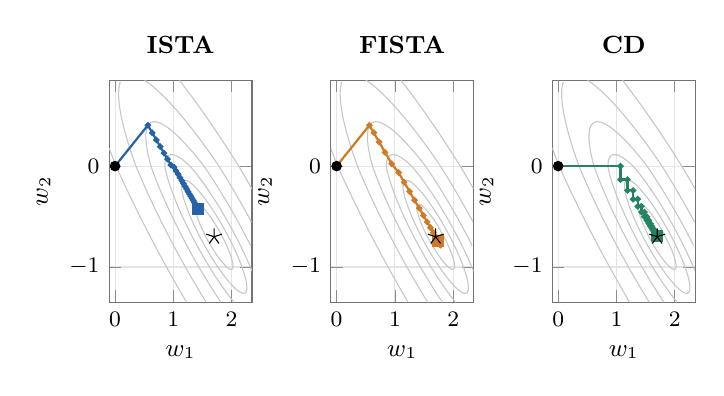
\begin{tikzpicture}
\begin{groupplot}[group style={group size=3 by 1,horizontal sep=1.0cm},width=.28\linewidth,height=4.4cm,xmin=-.1,xmax=2.35,ymin=-1.35,ymax=.85,xtick={0,1,2},ytick={-1,0},xlabel={$w_1$},ylabel={$w_2$},grid=major]
\nextgroupplot[title={ISTA}]
\addplot[black!22,thin] coordinates {(1.9696347,-1.0211989) (1.9584475,-1.0180713) (1.9360731,-1.0094312) (1.9248858,-1.0042128) (1.9131052,-0.99840183) (1.8949111,-0.98835616) (1.880137,-0.97969305) (1.8689498,-0.97268551) (1.8577626,-0.96548071) (1.8465753,-0.95807876) (1.8323981,-0.94817352) (1.8184255,-0.93812785) (1.804818,-0.92808219) (1.7915523,-0.91803653) (1.7794521,-0.90860113) (1.7682648,-0.8996426) (1.7570776,-0.89051572) (1.7458904,-0.88122059) (1.7347032,-0.87175727) (1.723516,-0.86212585) (1.7123288,-0.85232642) (1.7011416,-0.84235905) (1.6899543,-0.83222382) (1.6787671,-0.82192082) (1.6675799,-0.81145013) (1.6563927,-0.80081183) (1.6452055,-0.79000599) (1.6340183,-0.77903271) (1.6228311,-0.76789205) (1.612406,-0.75730594) (1.6026929,-0.74726027) (1.5931056,-0.73721461) (1.5836385,-0.72716895) (1.5742861,-0.71712329) (1.5650433,-0.70707763) (1.5557078,-0.69679326) (1.5445205,-0.6841102) (1.5333333,-0.67123309) (1.5221461,-0.65816203) (1.5126741,-0.64680365) (1.5044836,-0.63675799) (1.4963711,-0.62671233) (1.4883332,-0.61666667) (1.4773973,-0.60242219) (1.46621,-0.58759644) (1.4581602,-0.57648402) (1.4510238,-0.56643836) (1.4438356,-0.55623088) (1.4326484,-0.53937093) (1.4242954,-0.52625571) (1.4181588,-0.51621005) (1.410274,-0.50271648) (1.4012335,-0.48607306) (1.3962236,-0.4760274) (1.3878995,-0.45756738) (1.3835425,-0.44589041) (1.37769,-0.42579909) (1.3760477,-0.41575342) (1.3767123,-0.39786598) (1.3825621,-0.38561644) (1.3990868,-0.37637362) (1.4214612,-0.37687427) (1.4438356,-0.38278186) (1.4550228,-0.38685746) (1.4748821,-0.3956621) (1.4885845,-0.40255363) (1.4997717,-0.40861042) (1.512265,-0.41575342) (1.5286122,-0.42579909) (1.5443603,-0.43584475) (1.5557078,-0.44354283) (1.566895,-0.45133064) (1.5780822,-0.45930313) (1.5892694,-0.46746021) (1.6007278,-0.4760274) (1.613701,-0.48607306) (1.6263932,-0.49611872) (1.6388202,-0.50616438) (1.6509969,-0.51621005) (1.6629368,-0.52625571) (1.6746525,-0.53630137) (1.6861558,-0.54634703) (1.6974577,-0.55639269) (1.7085684,-0.56643836) (1.7194975,-0.57648402) (1.7302537,-0.58652968) (1.7408456,-0.59657534) (1.7512808,-0.606621) (1.7615668,-0.61666667) (1.7717103,-0.62671233) (1.7817179,-0.63675799) (1.7915957,-0.64680365) (1.8018265,-0.65738719) (1.8130137,-0.66921563) (1.8242009,-0.68122662) (1.8353881,-0.69342006) (1.8465753,-0.70579587) (1.8565938,-0.71712329) (1.8652788,-0.72716895) (1.8738713,-0.73721461) (1.8823756,-0.74726027) (1.8913242,-0.75800543) (1.9025114,-0.77188389) (1.9136986,-0.78597712) (1.922549,-0.79748858) (1.9300916,-0.80753425) (1.9375743,-0.81757991) (1.9472603,-0.83109558) (1.9584475,-0.84714229) (1.9654438,-0.85776256) (1.9719776,-0.86780822) (1.9808219,-0.88208695) (1.9901231,-0.89794521) (1.9956043,-0.90799087) (2.0031963,-0.9227916) (2.0102151,-0.93812785) (2.0144451,-0.94817352) (2.0207846,-0.96826484) (2.0242393,-0.98835616) (2.0211164,-1.0084475) (2.0134197,-1.0184932) (1.9920091,-1.0242421) (1.9696347,-1.0211989) (1.9696347,-1.0211989)};
\addplot[black!22,thin] coordinates {(2.1821918,-1.2597567) (2.1486301,-1.2512283) (2.1171362,-1.2394977) (2.0926941,-1.2286179) (2.0591324,-1.2115731) (2.036758,-1.1991726) (2.0033817,-1.1792237) (1.9808219,-1.1648521) (1.9569818,-1.1490868) (1.9279566,-1.1289954) (1.9025114,-1.1107182) (1.880137,-1.094092) (1.8577626,-1.077054) (1.8342729,-1.0586758) (1.8093015,-1.0385845) (1.7849125,-1.0184932) (1.7610695,-0.99840183) (1.7377391,-0.9783105) (1.7148904,-0.95821918) (1.6924951,-0.93812785) (1.670527,-0.91803653) (1.648962,-0.89794521) (1.6277776,-0.87785388) (1.6069531,-0.85776256) (1.5864691,-0.83767123) (1.5663078,-0.81757991) (1.5445205,-0.79542029) (1.5221461,-0.77223456) (1.4997717,-0.74864092) (1.4798331,-0.72716895) (1.4615026,-0.70707763) (1.4434137,-0.6869863) (1.4214612,-0.66199758) (1.3997027,-0.63675799) (1.3828233,-0.61666667) (1.3655251,-0.59578918) (1.3431507,-0.56802262) (1.326164,-0.54634703) (1.309589,-0.52477607) (1.2882713,-0.49611872) (1.273816,-0.4760274) (1.253653,-0.44707158) (1.2394668,-0.42579909) (1.2201811,-0.3956621) (1.208032,-0.37557078) (1.1909329,-0.34543379) (1.1753425,-0.31554162) (1.1641553,-0.29137097) (1.152968,-0.26362886) (1.1417808,-0.22565952) (1.1381772,-0.19474886) (1.1438581,-0.16461187) (1.1641553,-0.14398165) (1.2089041,-0.13905284) (1.2424658,-0.14604727) (1.2760274,-0.15772236) (1.309589,-0.17249659) (1.3338623,-0.1847032) (1.3655251,-0.20218681) (1.3878995,-0.21542554) (1.4188529,-0.23493151) (1.4438356,-0.25148613) (1.46621,-0.26687819) (1.4918008,-0.28515982) (1.518989,-0.30525114) (1.5445205,-0.32469458) (1.566895,-0.34227268) (1.5892694,-0.36024833) (1.6116438,-0.3786213) (1.6340183,-0.39739136) (1.6563927,-0.4165583) (1.6787671,-0.43612188) (1.7011416,-0.45608187) (1.723516,-0.47643806) (1.7458904,-0.49719021) (1.7682648,-0.5183381) (1.7906393,-0.5398815) (1.8130137,-0.56182019) (1.8353881,-0.58415395) (1.8574964,-0.606621) (1.8768445,-0.62671233) (1.8959102,-0.64680365) (1.914708,-0.66689498) (1.9360731,-0.69022906) (1.9584475,-0.71513343) (1.9778545,-0.73721461) (1.995195,-0.75730594) (2.0143836,-0.779963) (2.036758,-0.80700109) (2.0533457,-0.82762557) (2.0703196,-0.84908072) (2.0924194,-0.87785388) (2.1073419,-0.89794521) (2.1262557,-0.9240871) (2.1430528,-0.94817352) (2.1598174,-0.97311347) (2.1760483,-0.99840183) (2.193379,-1.0268426) (2.2058456,-1.0486301) (2.2217512,-1.0787671) (2.2359782,-1.1089041) (2.2479868,-1.1390411) (2.2569772,-1.1691781) (2.2617133,-1.1993151) (2.2584874,-1.2294521) (2.2381279,-1.2547018) (2.2045662,-1.2618629) (2.1821918,-1.2597567)};
\addplot[black!22,thin] coordinates {(2.0406713,-1.35) (2.0127617,-1.3299087) (1.9808219,-1.3062838) (1.9472603,-1.2808269) (1.9199533,-1.259589) (1.8913242,-1.2369188) (1.8577626,-1.2097731) (1.8329412,-1.1892694) (1.8018265,-1.1631351) (1.773664,-1.1390411) (1.7458904,-1.1148995) (1.7163933,-1.0888128) (1.6899543,-1.0650678) (1.6609408,-1.0385845) (1.6340183,-1.0136414) (1.6071407,-0.98835616) (1.5780822,-0.96062176) (1.5548471,-0.93812785) (1.5242017,-0.90799087) (1.4997717,-0.88360483) (1.4742287,-0.85776256) (1.4448701,-0.82762557) (1.4214612,-0.80319967) (1.3970409,-0.77739726) (1.3689717,-0.74726027) (1.3431507,-0.71911358) (1.3207763,-0.69434158) (1.2963432,-0.66689498) (1.269975,-0.63675799) (1.2440339,-0.606621) (1.2200913,-0.57828504) (1.1977169,-0.55132614) (1.1753425,-0.5239189) (1.152968,-0.49601586) (1.1294074,-0.46598174) (1.1062768,-0.43584475) (1.0836758,-0.40570776) (1.061626,-0.37557078) (1.04015,-0.34543379) (1.0187215,-0.31445773) (0.99634703,-0.28095803) (0.9739726,-0.24616856) (0.95472599,-0.21484018) (0.93702935,-0.1847032) (0.91803653,-0.15049555) (0.89942702,-0.11438356) (0.88447489,-0.082739441) (0.86836672,-0.044063927) (0.85462836,-0.0038812785) (0.85923714,0.046347032) (0.87364237,0.076484018) (0.90684932,0.10347281) (0.95159817,0.11439727) (1.0075342,0.11157738) (1.0522831,0.10206795) (1.097032,0.088263534) (1.1305936,0.07572191) (1.1753425,0.05662502) (1.2089041,0.040752881) (1.2424658,0.023793575) (1.2760274,0.0058125198) (1.309589,-0.01542258) (1.3431507,-0.038570837) (1.3767123,-0.062446349) (1.4064614,-0.084246575) (1.4333081,-0.1043379) (1.46621,-0.12960318) (1.4980018,-0.15456621) (1.5230858,-0.17465753) (1.5557078,-0.20132628) (1.583973,-0.22488584) (1.6116438,-0.24833128) (1.642684,-0.27511416) (1.6675799,-0.29694244) (1.6994294,-0.32534247) (1.723516,-0.34715826) (1.7543933,-0.37557078) (1.7794521,-0.39897727) (1.8077378,-0.42579909) (1.8353881,-0.45239798) (1.8596056,-0.4760274) (1.8900318,-0.50616438) (1.9136986,-0.52997574) (1.9396092,-0.55639269) (1.9687466,-0.58652968) (1.9920091,-0.6109929) (2.0162082,-0.63675799) (2.0440549,-0.66689498) (2.0703196,-0.69574835) (2.0926941,-0.72074298) (2.1161182,-0.74726027) (2.1422581,-0.77739726) (2.1679656,-0.80753425) (2.193224,-0.83767123) (2.2157534,-0.86511306) (2.2381279,-0.8928459) (2.2605023,-0.92110126) (2.2828767,-0.94993691) (2.3052511,-0.97941943) (2.3276256,-1.009626) (2.35,-1.0406467)};
\addplot[black!22,thin] coordinates {(1.8162793,-1.35) (1.7814548,-1.319863) (1.7471107,-1.289726) (1.7132281,-1.259589) (1.6797887,-1.2294521) (1.6467754,-1.1993151) (1.6141719,-1.1691781) (1.5819627,-1.1390411) (1.5501332,-1.1089041) (1.5186693,-1.0787671) (1.4875577,-1.0486301) (1.4550228,-1.0167195) (1.4214612,-0.98338795) (1.3878995,-0.9496565) (1.3568391,-0.91803653) (1.3275729,-0.88789954) (1.2984018,-0.85755543) (1.2648402,-0.82216137) (1.2323135,-0.78744292) (1.2044501,-0.75730594) (1.1753425,-0.72548833) (1.1417808,-0.68829907) (1.1137935,-0.65684932) (1.0858447,-0.6250896) (1.052393,-0.58652968) (1.0266434,-0.55639269) (0.99634703,-0.52047561) (0.96776789,-0.48607306) (0.94041096,-0.4526639) (0.91067967,-0.41575342) (0.88447489,-0.38269725) (0.85545388,-0.34543379) (0.82853881,-0.31024836) (0.80216996,-0.27511416) (0.77261122,-0.23493151) (0.75022831,-0.20381182) (0.72266386,-0.16461187) (0.69511056,-0.12442922) (0.67191781,-0.089613024) (0.64887965,-0.054109589) (0.6236869,-0.013926941) (0.60295457,0.026255708) (0.58242009,0.073848896) (0.56593941,0.11666667) (0.54941584,0.16689498) (0.53767123,0.21293572) (0.52921934,0.2673516) (0.5301582,0.32762557) (0.54582102,0.37785388) (0.57123288,0.40950786) (0.61598174,0.4329472) (0.67191781,0.44046129) (0.72785388,0.43591115) (0.78378995,0.4239372) (0.83607969,0.40799087) (0.88447489,0.39007444) (0.92922374,0.37125454) (0.9739726,0.35060773) (1.0187215,0.32836469) (1.0581548,0.30753425) (1.097032,0.28604883) (1.1417808,0.2601676) (1.1799468,0.23721461) (1.2200913,0.21227447) (1.2595516,0.1869863) (1.2984018,0.16140173) (1.3349045,0.13675799) (1.3767123,0.10786113) (1.410274,0.084142217) (1.4487781,0.056392694) (1.4885845,0.027154665) (1.5221461,0.0018638095) (1.5557078,-0.026052818) (1.5892694,-0.054756284) (1.6232697,-0.084246575) (1.6575364,-0.11438356) (1.6913529,-0.14452055) (1.7247365,-0.17465753) (1.7577036,-0.20479452) (1.7906393,-0.2352827) (1.8242009,-0.2667533) (1.8577626,-0.29861861) (1.8913242,-0.33087848) (1.9248858,-0.36353275) (1.9575018,-0.3956621) (1.9877143,-0.42579909) (2.0176101,-0.45593607) (2.0479452,-0.48685204) (2.0815068,-0.52151248) (2.1148854,-0.55639269) (2.1433329,-0.58652968) (2.1715118,-0.61666667) (2.2045662,-0.65250846) (2.235963,-0.6869863) (2.2630625,-0.71712329) (2.2940639,-0.75203806) (2.3250732,-0.78744292)};
\addplot[black!22,thin] coordinates {(1.5640967,-1.35) (1.5445205,-1.3316852) (1.531941,-1.319863) (1.5109589,-1.3000625) (1.4997717,-1.2894568) (1.4789594,-1.2696347) (1.46621,-1.2574419) (1.4475294,-1.2394977) (1.4326484,-1.2251477) (1.4163507,-1.2093607) (1.3990868,-1.1925741) (1.3854168,-1.1792237) (1.3655251,-1.1597212) (1.3543379,-1.1487032) (1.3344234,-1.1289954) (1.3207763,-1.115437) (1.30416,-1.0988584) (1.2872146,-1.0818881) (1.2741219,-1.0687215) (1.2542273,-1.0486301) (1.2424658,-1.0366912) (1.2246093,-1.0184932) (1.2089041,-1.0024279) (1.195204,-0.98835616) (1.1757215,-0.96826484) (1.1641553,-0.95627179) (1.1467245,-0.93812785) (1.1305936,-0.92127498) (1.1179284,-0.90799087) (1.0988663,-0.88789954) (1.0858447,-0.87411029) (1.0704672,-0.85776256) (1.0522831,-0.8383602) (1.0410959,-0.82636069) (1.0236236,-0.80753425) (1.0075342,-0.79013454) (0.99579966,-0.77739726) (0.97739871,-0.75730594) (0.96278539,-0.74128586) (0.94995604,-0.72716895) (0.93179363,-0.70707763) (0.91803653,-0.69178741) (0.90472754,-0.67694064) (0.88680945,-0.65684932) (0.87328767,-0.64161091) (0.86011524,-0.62671233) (0.84244728,-0.606621) (0.82853881,-0.5907264) (0.81612023,-0.57648402) (0.79870822,-0.55639269) (0.78378995,-0.53910211) (0.77260274,-0.52608892) (0.75559338,-0.50616438) (0.7390411,-0.48670438) (0.72785388,-0.47346489) (0.71310387,-0.45593607) (0.69628124,-0.43584475) (0.68310502,-0.42001183) (0.6712408,-0.40570776) (0.6546967,-0.38561644) (0.63835616,-0.36569019) (0.62716895,-0.35194161) (0.61374573,-0.33538813) (0.59755811,-0.3152968) (0.58242009,-0.29640913) (0.57123288,-0.28235519) (0.55753781,-0.26506849) (0.54172557,-0.24497717) (0.52648402,-0.22550358) (0.5152968,-0.21109484) (0.50265503,-0.19474886) (0.48723798,-0.17465753) (0.47191085,-0.15456621) (0.45936073,-0.13798013) (0.44817352,-0.12312465) (0.43413586,-0.1043379) (0.4192335,-0.084246575) (0.40443273,-0.064155251) (0.39223744,-0.04744797) (0.38105023,-0.032035368) (0.36800616,-0.013926941) (0.35418221,0.0061643836) (0.34166916,0.026255708) (0.329308,0.046347032) (0.31710327,0.066438356) (0.3050597,0.08652968) (0.29318223,0.106621) (0.28147599,0.12671233) (0.2699463,0.14680365) (0.25859874,0.16689498) (0.24743911,0.1869863) (0.23647346,0.20707763) (0.2257081,0.22716895) (0.21514963,0.24726027) (0.20480492,0.2673516) (0.19468118,0.28744292) (0.18478591,0.30753425) (0.17512698,0.32762557) (0.16571262,0.34771689) (0.15655144,0.36780822) (0.14611872,0.3915243) (0.13493151,0.41795737) (0.12678948,0.43812785) (0.11899017,0.45821918) (0.11151187,0.4783105) (0.10136986,0.5073876) (0.094537978,0.52853881) (0.088458954,0.54863014) (0.080239718,0.57876712) (0.075425081,0.59885845) (0.069251373,0.62899543) (0.065958072,0.64908676) (0.062424911,0.67922374) (0.060831794,0.70936073) (0.061639982,0.73949772) (0.06546955,0.7696347) (0.070199954,0.78972603) (0.078995434,0.81402293) (0.090182648,0.8348741)};
\addplot[black!22,thin] coordinates {(0.50870251,0.85) (0.53450149,0.83995434) (0.55905454,0.82990868) (0.58242009,0.81992438) (0.60479452,0.80999291) (0.62707454,0.79977169) (0.64830832,0.78972603) (0.66898333,0.77968037) (0.68917136,0.7696347) (0.70893238,0.75958904) (0.72831693,0.74954338) (0.75022831,0.73792651) (0.77260274,0.72581443) (0.79497717,0.71346709) (0.8173516,0.70089511) (0.83767263,0.68926941) (0.85497525,0.67922374) (0.87328767,0.66847692) (0.8956621,0.65512405) (0.91803653,0.64158526) (0.93855308,0.62899543) (0.95472728,0.61894977) (0.9739726,0.6068816) (0.99634703,0.59266754) (1.0179844,0.57876712) (1.0334318,0.56872146) (1.0522831,0.55637324) (1.0746575,0.54155168) (1.0940977,0.52853881) (1.1089992,0.51849315) (1.1305936,0.50378228) (1.152968,0.48841317) (1.1675144,0.4783105) (1.1865297,0.46503176) (1.2089041,0.44927277) (1.2245756,0.43812785) (1.2424658,0.42533892) (1.2648402,0.40921235) (1.2803342,0.39794521) (1.2984018,0.38474049) (1.3207763,0.36826732) (1.3349212,0.35776256) (1.3543379,0.34327135) (1.3751597,0.32762557) (1.3884508,0.31757991) (1.410274,0.3009646) (1.4279196,0.28744292) (1.4438356,0.27519017) (1.46621,0.25785169) (1.4797793,0.24726027) (1.4997717,0.23158278) (1.5180985,0.21712329) (1.5333333,0.20504967) (1.5557078,0.1872114) (1.5685049,0.17694064) (1.5892694,0.16019944) (1.6057897,0.14680365) (1.6228311,0.1329267) (1.6426863,0.11666667) (1.6563927,0.10539322) (1.6787671,0.086888374) (1.691275,0.076484018) (1.7123288,0.058894323) (1.7272684,0.046347032) (1.7458904,0.030642867) (1.7629149,0.016210046) (1.7794521,0.002018646) (1.797053,-0.013926941) (1.8130137,-0.028699935) (1.8295331,-0.044063927) (1.8465753,-0.05997645) (1.8617378,-0.074200913) (1.880137,-0.091529681) (1.8936744,-0.1043379) (1.9136986,-0.12335956) (1.9253499,-0.13447489) (1.9463108,-0.15456621) (1.9584475,-0.16625089) (1.9775312,-0.1847032) (1.9920091,-0.19875676) (2.0085049,-0.21484018) (2.0255708,-0.23154266) (2.0392382,-0.24497717) (2.0591324,-0.26460852) (2.0703196,-0.27570039) (2.089902,-0.29520548) (2.1038813,-0.30918344) (2.1199735,-0.32534247) (2.1374429,-0.34294999) (2.1498237,-0.35547945) (2.169583,-0.37557078) (2.1821918,-0.38845073) (2.1990173,-0.40570776) (2.2157534,-0.42293647) (2.2282429,-0.43584475) (2.2475881,-0.45593607) (2.2605023,-0.4694103) (2.2764093,-0.48607306) (2.2940639,-0.50463445) (2.3052511,-0.51644366) (2.3239565,-0.53630137) (2.3388128,-0.55213152)};
\addplot[black!22,thin] coordinates {(1.2268436,-1.35) (1.2089041,-1.3323313) (1.1962825,-1.319863) (1.1760065,-1.2997717) (1.1641553,-1.2879878) (1.1457507,-1.2696347) (1.1305936,-1.2544796) (1.1156549,-1.2394977) (1.097032,-1.2207712) (1.0857162,-1.2093607) (1.0658678,-1.1892694) (1.0522831,-1.1754802) (1.0362249,-1.1591324) (1.0187215,-1.1412666) (1.0067328,-1.1289954) (0.98717466,-1.1089041) (0.9739726,-1.0953007) (0.95797257,-1.0787671) (0.94041096,-1.0605725) (0.9289153,-1.0486301) (0.90965163,-1.0285388) (0.8956621,-1.0139074) (0.8808786,-0.99840183) (0.86210046,-0.9786548) (0.85091324,-0.9668445) (0.83327941,-0.94817352) (0.8173516,-0.93126511) (0.80492399,-0.91803653) (0.7861183,-0.89794521) (0.77260274,-0.88345967) (0.75803915,-0.86780822) (0.7393958,-0.84771689) (0.72785388,-0.83522614) (0.71159058,-0.81757991) (0.69429224,-0.79876226) (0.68310502,-0.78655173) (0.66557882,-0.7673516) (0.64954338,-0.74973929) (0.63816909,-0.73721461) (0.62000443,-0.71712329) (0.60479452,-0.7002551) (0.5928608,-0.6869863) (0.57486794,-0.66689498) (0.56004566,-0.65029562) (0.54798808,-0.63675799) (0.53016992,-0.61666667) (0.5152968,-0.59984617) (0.50355148,-0.58652968) (0.4859109,-0.56643836) (0.47054795,-0.54889148) (0.45936073,-0.53608017) (0.44209145,-0.51621005) (0.42579909,-0.49741563) (0.41461187,-0.48446046) (0.39871211,-0.46598174) (0.38147256,-0.44589041) (0.36986301,-0.43229411) (0.35577343,-0.41575342) (0.3387226,-0.3956621) (0.32511416,-0.37956333) (0.31327597,-0.36552511) (0.29641682,-0.34543379) (0.2803653,-0.32624956) (0.26917808,-0.31281759) (0.25455578,-0.29520548) (0.23793654,-0.27511416) (0.22442922,-0.25871501) (0.21314006,-0.24497717) (0.196721,-0.22488584) (0.18035066,-0.20479452) (0.16849315,-0.1901641) (0.15595436,-0.17465753) (0.13978989,-0.15456621) (0.12374429,-0.13455718) (0.11255708,-0.120525) (0.099681657,-0.1043379) (0.083781226,-0.084246575) (0.067936984,-0.064155251) (0.056621005,-0.049718949) (0.044340929,-0.034018265) (0.028714324,-0.013926941) (0.013501172,0.0061643836) (0.00068493151,0.024132244) (-0.010502283,0.040753778) (-0.021689498,0.057506856) (-0.034276956,0.076484018) (-0.047510771,0.096575342) (-0.060656162,0.11666667) (-0.073711436,0.13675799) (-0.086674852,0.15684932) (-0.099544627,0.17694064)};
\addplot[black!22,thin] coordinates {(1.1059399,0.85) (1.1194064,0.83996124) (1.1305936,0.83158003) (1.1417808,0.82317678) (1.152968,0.8147515) (1.1641553,0.80630418) (1.1753425,0.79783483) (1.1865297,0.78934345) (1.1992074,0.77968037) (1.2123439,0.7696347) (1.225442,0.75958904) (1.2385021,0.74954338) (1.2515245,0.73949772) (1.2645095,0.72945205) (1.2760274,0.72050578) (1.2872146,0.71179146) (1.2984018,0.70305553) (1.309589,0.69429799) (1.3207763,0.68551883) (1.3319635,0.67671806) (1.3431507,0.66789568) (1.3543379,0.65905169) (1.3668948,0.64908676) (1.3795187,0.6390411) (1.3921089,0.62899543) (1.4046656,0.61894977) (1.4171892,0.60890411) (1.4296799,0.59885845) (1.4421378,0.58881279) (1.4545633,0.57876712) (1.46621,0.56932116) (1.4773973,0.56022232) (1.4885845,0.55110226) (1.4997717,0.54196101) (1.5109589,0.53279854) (1.5221461,0.52361488) (1.5333333,0.51441001) (1.5445205,0.50518395) (1.5557078,0.49593668) (1.566895,0.48666822) (1.5780822,0.47737856) (1.5892694,0.46806771) (1.6010685,0.45821918) (1.6130728,0.44817352) (1.6250485,0.43812785) (1.6369957,0.42808219) (1.6489147,0.41803653) (1.6608056,0.40799087) (1.6726686,0.39794521) (1.6845039,0.38789954) (1.6963117,0.37785388) (1.7080922,0.36780822) (1.7198456,0.35776256) (1.731572,0.34771689) (1.7432716,0.33767123) (1.7549446,0.32762557) (1.7665911,0.31757991) (1.7782114,0.30753425) (1.7898057,0.29748858) (1.801374,0.28744292) (1.8129165,0.27739726) (1.8242009,0.26755267) (1.8353881,0.25777114) (1.8465753,0.24796881) (1.8577626,0.23814569) (1.8689498,0.22830178) (1.880137,0.21843708) (1.8913242,0.20855159) (1.9025114,0.19864531) (1.9136986,0.18871825) (1.9248858,0.17877041) (1.9360731,0.16880178) (1.9472603,0.15881237) (1.9584475,0.14880217) (1.9696347,0.1387712) (1.9808219,0.12871945) (1.9920091,0.11864692) (2.0031963,0.10855362) (2.0143836,0.09843954) (2.0255708,0.088304688) (2.036758,0.078149064) (2.0479452,0.067972669) (2.0591324,0.057775504) (2.0703196,0.04755757) (2.0815068,0.03731887) (2.0926941,0.027059403) (2.1038813,0.016779171) (2.1150685,0.0064781762) (2.1260745,-0.0038812785) (2.1363638,-0.013926941) (2.1466342,-0.023972603) (2.1568857,-0.034018265) (2.1671185,-0.044063927) (2.1773327,-0.054109589) (2.1875284,-0.064155251) (2.1977057,-0.074200913) (2.2078648,-0.084246575) (2.2180057,-0.094292237) (2.2281285,-0.1043379) (2.2382334,-0.11438356) (2.2493151,-0.12543127) (2.2605023,-0.13660741) (2.2716895,-0.14780582) (2.2828767,-0.15902652) (2.2940639,-0.17026949) (2.3052511,-0.18153474) (2.3164384,-0.19282227) (2.3276256,-0.20413206) (2.3381916,-0.21484018) (2.3480798,-0.22488584)};
\addplot[lassoblue,thick,mark=*,mark size=.7pt] coordinates {(0,0) (0.56315789,0.40526316) (0.63795014,0.33047091) (0.70880595,0.2596151) (0.77593251,0.19248855) (0.83952609,0.12889497) (0.89977263,0.068648418) (0.95684831,0.011572739) (1.01092,-0.010920009) (1.0471874,-0.047187377) (1.0815459,-0.081545936) (1.1140961,-0.11409615) (1.1449332,-0.14493319) (1.1741472,-0.17414724) (1.2018237,-0.2018237) (1.2280435,-0.2280435) (1.2528833,-0.25288332) (1.2764158,-0.27641578) (1.2987097,-0.29870968) (1.3198302,-0.31983023) (1.3398392,-0.33983916) (1.358795,-0.35879499) (1.3767532,-0.37675315) (1.3937661,-0.39376614) (1.4098837,-0.40988372) (1.425153,-0.42515299)};
\addplot[lassoblue,only marks,mark=square*,mark size=2pt] coordinates {(1.425153,-0.42515299)};
\addplot[black,only marks,mark=*,mark size=1.7pt] coordinates {(0,0)};
\addplot[black,only marks,mark=star,mark size=3pt] coordinates {(1.7,-0.7)};
\nextgroupplot[title={FISTA}]
\addplot[black!22,thin] coordinates {(1.9696347,-1.0211989) (1.9584475,-1.0180713) (1.9360731,-1.0094312) (1.9248858,-1.0042128) (1.9131052,-0.99840183) (1.8949111,-0.98835616) (1.880137,-0.97969305) (1.8689498,-0.97268551) (1.8577626,-0.96548071) (1.8465753,-0.95807876) (1.8323981,-0.94817352) (1.8184255,-0.93812785) (1.804818,-0.92808219) (1.7915523,-0.91803653) (1.7794521,-0.90860113) (1.7682648,-0.8996426) (1.7570776,-0.89051572) (1.7458904,-0.88122059) (1.7347032,-0.87175727) (1.723516,-0.86212585) (1.7123288,-0.85232642) (1.7011416,-0.84235905) (1.6899543,-0.83222382) (1.6787671,-0.82192082) (1.6675799,-0.81145013) (1.6563927,-0.80081183) (1.6452055,-0.79000599) (1.6340183,-0.77903271) (1.6228311,-0.76789205) (1.612406,-0.75730594) (1.6026929,-0.74726027) (1.5931056,-0.73721461) (1.5836385,-0.72716895) (1.5742861,-0.71712329) (1.5650433,-0.70707763) (1.5557078,-0.69679326) (1.5445205,-0.6841102) (1.5333333,-0.67123309) (1.5221461,-0.65816203) (1.5126741,-0.64680365) (1.5044836,-0.63675799) (1.4963711,-0.62671233) (1.4883332,-0.61666667) (1.4773973,-0.60242219) (1.46621,-0.58759644) (1.4581602,-0.57648402) (1.4510238,-0.56643836) (1.4438356,-0.55623088) (1.4326484,-0.53937093) (1.4242954,-0.52625571) (1.4181588,-0.51621005) (1.410274,-0.50271648) (1.4012335,-0.48607306) (1.3962236,-0.4760274) (1.3878995,-0.45756738) (1.3835425,-0.44589041) (1.37769,-0.42579909) (1.3760477,-0.41575342) (1.3767123,-0.39786598) (1.3825621,-0.38561644) (1.3990868,-0.37637362) (1.4214612,-0.37687427) (1.4438356,-0.38278186) (1.4550228,-0.38685746) (1.4748821,-0.3956621) (1.4885845,-0.40255363) (1.4997717,-0.40861042) (1.512265,-0.41575342) (1.5286122,-0.42579909) (1.5443603,-0.43584475) (1.5557078,-0.44354283) (1.566895,-0.45133064) (1.5780822,-0.45930313) (1.5892694,-0.46746021) (1.6007278,-0.4760274) (1.613701,-0.48607306) (1.6263932,-0.49611872) (1.6388202,-0.50616438) (1.6509969,-0.51621005) (1.6629368,-0.52625571) (1.6746525,-0.53630137) (1.6861558,-0.54634703) (1.6974577,-0.55639269) (1.7085684,-0.56643836) (1.7194975,-0.57648402) (1.7302537,-0.58652968) (1.7408456,-0.59657534) (1.7512808,-0.606621) (1.7615668,-0.61666667) (1.7717103,-0.62671233) (1.7817179,-0.63675799) (1.7915957,-0.64680365) (1.8018265,-0.65738719) (1.8130137,-0.66921563) (1.8242009,-0.68122662) (1.8353881,-0.69342006) (1.8465753,-0.70579587) (1.8565938,-0.71712329) (1.8652788,-0.72716895) (1.8738713,-0.73721461) (1.8823756,-0.74726027) (1.8913242,-0.75800543) (1.9025114,-0.77188389) (1.9136986,-0.78597712) (1.922549,-0.79748858) (1.9300916,-0.80753425) (1.9375743,-0.81757991) (1.9472603,-0.83109558) (1.9584475,-0.84714229) (1.9654438,-0.85776256) (1.9719776,-0.86780822) (1.9808219,-0.88208695) (1.9901231,-0.89794521) (1.9956043,-0.90799087) (2.0031963,-0.9227916) (2.0102151,-0.93812785) (2.0144451,-0.94817352) (2.0207846,-0.96826484) (2.0242393,-0.98835616) (2.0211164,-1.0084475) (2.0134197,-1.0184932) (1.9920091,-1.0242421) (1.9696347,-1.0211989) (1.9696347,-1.0211989)};
\addplot[black!22,thin] coordinates {(2.1821918,-1.2597567) (2.1486301,-1.2512283) (2.1171362,-1.2394977) (2.0926941,-1.2286179) (2.0591324,-1.2115731) (2.036758,-1.1991726) (2.0033817,-1.1792237) (1.9808219,-1.1648521) (1.9569818,-1.1490868) (1.9279566,-1.1289954) (1.9025114,-1.1107182) (1.880137,-1.094092) (1.8577626,-1.077054) (1.8342729,-1.0586758) (1.8093015,-1.0385845) (1.7849125,-1.0184932) (1.7610695,-0.99840183) (1.7377391,-0.9783105) (1.7148904,-0.95821918) (1.6924951,-0.93812785) (1.670527,-0.91803653) (1.648962,-0.89794521) (1.6277776,-0.87785388) (1.6069531,-0.85776256) (1.5864691,-0.83767123) (1.5663078,-0.81757991) (1.5445205,-0.79542029) (1.5221461,-0.77223456) (1.4997717,-0.74864092) (1.4798331,-0.72716895) (1.4615026,-0.70707763) (1.4434137,-0.6869863) (1.4214612,-0.66199758) (1.3997027,-0.63675799) (1.3828233,-0.61666667) (1.3655251,-0.59578918) (1.3431507,-0.56802262) (1.326164,-0.54634703) (1.309589,-0.52477607) (1.2882713,-0.49611872) (1.273816,-0.4760274) (1.253653,-0.44707158) (1.2394668,-0.42579909) (1.2201811,-0.3956621) (1.208032,-0.37557078) (1.1909329,-0.34543379) (1.1753425,-0.31554162) (1.1641553,-0.29137097) (1.152968,-0.26362886) (1.1417808,-0.22565952) (1.1381772,-0.19474886) (1.1438581,-0.16461187) (1.1641553,-0.14398165) (1.2089041,-0.13905284) (1.2424658,-0.14604727) (1.2760274,-0.15772236) (1.309589,-0.17249659) (1.3338623,-0.1847032) (1.3655251,-0.20218681) (1.3878995,-0.21542554) (1.4188529,-0.23493151) (1.4438356,-0.25148613) (1.46621,-0.26687819) (1.4918008,-0.28515982) (1.518989,-0.30525114) (1.5445205,-0.32469458) (1.566895,-0.34227268) (1.5892694,-0.36024833) (1.6116438,-0.3786213) (1.6340183,-0.39739136) (1.6563927,-0.4165583) (1.6787671,-0.43612188) (1.7011416,-0.45608187) (1.723516,-0.47643806) (1.7458904,-0.49719021) (1.7682648,-0.5183381) (1.7906393,-0.5398815) (1.8130137,-0.56182019) (1.8353881,-0.58415395) (1.8574964,-0.606621) (1.8768445,-0.62671233) (1.8959102,-0.64680365) (1.914708,-0.66689498) (1.9360731,-0.69022906) (1.9584475,-0.71513343) (1.9778545,-0.73721461) (1.995195,-0.75730594) (2.0143836,-0.779963) (2.036758,-0.80700109) (2.0533457,-0.82762557) (2.0703196,-0.84908072) (2.0924194,-0.87785388) (2.1073419,-0.89794521) (2.1262557,-0.9240871) (2.1430528,-0.94817352) (2.1598174,-0.97311347) (2.1760483,-0.99840183) (2.193379,-1.0268426) (2.2058456,-1.0486301) (2.2217512,-1.0787671) (2.2359782,-1.1089041) (2.2479868,-1.1390411) (2.2569772,-1.1691781) (2.2617133,-1.1993151) (2.2584874,-1.2294521) (2.2381279,-1.2547018) (2.2045662,-1.2618629) (2.1821918,-1.2597567)};
\addplot[black!22,thin] coordinates {(2.0406713,-1.35) (2.0127617,-1.3299087) (1.9808219,-1.3062838) (1.9472603,-1.2808269) (1.9199533,-1.259589) (1.8913242,-1.2369188) (1.8577626,-1.2097731) (1.8329412,-1.1892694) (1.8018265,-1.1631351) (1.773664,-1.1390411) (1.7458904,-1.1148995) (1.7163933,-1.0888128) (1.6899543,-1.0650678) (1.6609408,-1.0385845) (1.6340183,-1.0136414) (1.6071407,-0.98835616) (1.5780822,-0.96062176) (1.5548471,-0.93812785) (1.5242017,-0.90799087) (1.4997717,-0.88360483) (1.4742287,-0.85776256) (1.4448701,-0.82762557) (1.4214612,-0.80319967) (1.3970409,-0.77739726) (1.3689717,-0.74726027) (1.3431507,-0.71911358) (1.3207763,-0.69434158) (1.2963432,-0.66689498) (1.269975,-0.63675799) (1.2440339,-0.606621) (1.2200913,-0.57828504) (1.1977169,-0.55132614) (1.1753425,-0.5239189) (1.152968,-0.49601586) (1.1294074,-0.46598174) (1.1062768,-0.43584475) (1.0836758,-0.40570776) (1.061626,-0.37557078) (1.04015,-0.34543379) (1.0187215,-0.31445773) (0.99634703,-0.28095803) (0.9739726,-0.24616856) (0.95472599,-0.21484018) (0.93702935,-0.1847032) (0.91803653,-0.15049555) (0.89942702,-0.11438356) (0.88447489,-0.082739441) (0.86836672,-0.044063927) (0.85462836,-0.0038812785) (0.85923714,0.046347032) (0.87364237,0.076484018) (0.90684932,0.10347281) (0.95159817,0.11439727) (1.0075342,0.11157738) (1.0522831,0.10206795) (1.097032,0.088263534) (1.1305936,0.07572191) (1.1753425,0.05662502) (1.2089041,0.040752881) (1.2424658,0.023793575) (1.2760274,0.0058125198) (1.309589,-0.01542258) (1.3431507,-0.038570837) (1.3767123,-0.062446349) (1.4064614,-0.084246575) (1.4333081,-0.1043379) (1.46621,-0.12960318) (1.4980018,-0.15456621) (1.5230858,-0.17465753) (1.5557078,-0.20132628) (1.583973,-0.22488584) (1.6116438,-0.24833128) (1.642684,-0.27511416) (1.6675799,-0.29694244) (1.6994294,-0.32534247) (1.723516,-0.34715826) (1.7543933,-0.37557078) (1.7794521,-0.39897727) (1.8077378,-0.42579909) (1.8353881,-0.45239798) (1.8596056,-0.4760274) (1.8900318,-0.50616438) (1.9136986,-0.52997574) (1.9396092,-0.55639269) (1.9687466,-0.58652968) (1.9920091,-0.6109929) (2.0162082,-0.63675799) (2.0440549,-0.66689498) (2.0703196,-0.69574835) (2.0926941,-0.72074298) (2.1161182,-0.74726027) (2.1422581,-0.77739726) (2.1679656,-0.80753425) (2.193224,-0.83767123) (2.2157534,-0.86511306) (2.2381279,-0.8928459) (2.2605023,-0.92110126) (2.2828767,-0.94993691) (2.3052511,-0.97941943) (2.3276256,-1.009626) (2.35,-1.0406467)};
\addplot[black!22,thin] coordinates {(1.8162793,-1.35) (1.7814548,-1.319863) (1.7471107,-1.289726) (1.7132281,-1.259589) (1.6797887,-1.2294521) (1.6467754,-1.1993151) (1.6141719,-1.1691781) (1.5819627,-1.1390411) (1.5501332,-1.1089041) (1.5186693,-1.0787671) (1.4875577,-1.0486301) (1.4550228,-1.0167195) (1.4214612,-0.98338795) (1.3878995,-0.9496565) (1.3568391,-0.91803653) (1.3275729,-0.88789954) (1.2984018,-0.85755543) (1.2648402,-0.82216137) (1.2323135,-0.78744292) (1.2044501,-0.75730594) (1.1753425,-0.72548833) (1.1417808,-0.68829907) (1.1137935,-0.65684932) (1.0858447,-0.6250896) (1.052393,-0.58652968) (1.0266434,-0.55639269) (0.99634703,-0.52047561) (0.96776789,-0.48607306) (0.94041096,-0.4526639) (0.91067967,-0.41575342) (0.88447489,-0.38269725) (0.85545388,-0.34543379) (0.82853881,-0.31024836) (0.80216996,-0.27511416) (0.77261122,-0.23493151) (0.75022831,-0.20381182) (0.72266386,-0.16461187) (0.69511056,-0.12442922) (0.67191781,-0.089613024) (0.64887965,-0.054109589) (0.6236869,-0.013926941) (0.60295457,0.026255708) (0.58242009,0.073848896) (0.56593941,0.11666667) (0.54941584,0.16689498) (0.53767123,0.21293572) (0.52921934,0.2673516) (0.5301582,0.32762557) (0.54582102,0.37785388) (0.57123288,0.40950786) (0.61598174,0.4329472) (0.67191781,0.44046129) (0.72785388,0.43591115) (0.78378995,0.4239372) (0.83607969,0.40799087) (0.88447489,0.39007444) (0.92922374,0.37125454) (0.9739726,0.35060773) (1.0187215,0.32836469) (1.0581548,0.30753425) (1.097032,0.28604883) (1.1417808,0.2601676) (1.1799468,0.23721461) (1.2200913,0.21227447) (1.2595516,0.1869863) (1.2984018,0.16140173) (1.3349045,0.13675799) (1.3767123,0.10786113) (1.410274,0.084142217) (1.4487781,0.056392694) (1.4885845,0.027154665) (1.5221461,0.0018638095) (1.5557078,-0.026052818) (1.5892694,-0.054756284) (1.6232697,-0.084246575) (1.6575364,-0.11438356) (1.6913529,-0.14452055) (1.7247365,-0.17465753) (1.7577036,-0.20479452) (1.7906393,-0.2352827) (1.8242009,-0.2667533) (1.8577626,-0.29861861) (1.8913242,-0.33087848) (1.9248858,-0.36353275) (1.9575018,-0.3956621) (1.9877143,-0.42579909) (2.0176101,-0.45593607) (2.0479452,-0.48685204) (2.0815068,-0.52151248) (2.1148854,-0.55639269) (2.1433329,-0.58652968) (2.1715118,-0.61666667) (2.2045662,-0.65250846) (2.235963,-0.6869863) (2.2630625,-0.71712329) (2.2940639,-0.75203806) (2.3250732,-0.78744292)};
\addplot[black!22,thin] coordinates {(1.5640967,-1.35) (1.5445205,-1.3316852) (1.531941,-1.319863) (1.5109589,-1.3000625) (1.4997717,-1.2894568) (1.4789594,-1.2696347) (1.46621,-1.2574419) (1.4475294,-1.2394977) (1.4326484,-1.2251477) (1.4163507,-1.2093607) (1.3990868,-1.1925741) (1.3854168,-1.1792237) (1.3655251,-1.1597212) (1.3543379,-1.1487032) (1.3344234,-1.1289954) (1.3207763,-1.115437) (1.30416,-1.0988584) (1.2872146,-1.0818881) (1.2741219,-1.0687215) (1.2542273,-1.0486301) (1.2424658,-1.0366912) (1.2246093,-1.0184932) (1.2089041,-1.0024279) (1.195204,-0.98835616) (1.1757215,-0.96826484) (1.1641553,-0.95627179) (1.1467245,-0.93812785) (1.1305936,-0.92127498) (1.1179284,-0.90799087) (1.0988663,-0.88789954) (1.0858447,-0.87411029) (1.0704672,-0.85776256) (1.0522831,-0.8383602) (1.0410959,-0.82636069) (1.0236236,-0.80753425) (1.0075342,-0.79013454) (0.99579966,-0.77739726) (0.97739871,-0.75730594) (0.96278539,-0.74128586) (0.94995604,-0.72716895) (0.93179363,-0.70707763) (0.91803653,-0.69178741) (0.90472754,-0.67694064) (0.88680945,-0.65684932) (0.87328767,-0.64161091) (0.86011524,-0.62671233) (0.84244728,-0.606621) (0.82853881,-0.5907264) (0.81612023,-0.57648402) (0.79870822,-0.55639269) (0.78378995,-0.53910211) (0.77260274,-0.52608892) (0.75559338,-0.50616438) (0.7390411,-0.48670438) (0.72785388,-0.47346489) (0.71310387,-0.45593607) (0.69628124,-0.43584475) (0.68310502,-0.42001183) (0.6712408,-0.40570776) (0.6546967,-0.38561644) (0.63835616,-0.36569019) (0.62716895,-0.35194161) (0.61374573,-0.33538813) (0.59755811,-0.3152968) (0.58242009,-0.29640913) (0.57123288,-0.28235519) (0.55753781,-0.26506849) (0.54172557,-0.24497717) (0.52648402,-0.22550358) (0.5152968,-0.21109484) (0.50265503,-0.19474886) (0.48723798,-0.17465753) (0.47191085,-0.15456621) (0.45936073,-0.13798013) (0.44817352,-0.12312465) (0.43413586,-0.1043379) (0.4192335,-0.084246575) (0.40443273,-0.064155251) (0.39223744,-0.04744797) (0.38105023,-0.032035368) (0.36800616,-0.013926941) (0.35418221,0.0061643836) (0.34166916,0.026255708) (0.329308,0.046347032) (0.31710327,0.066438356) (0.3050597,0.08652968) (0.29318223,0.106621) (0.28147599,0.12671233) (0.2699463,0.14680365) (0.25859874,0.16689498) (0.24743911,0.1869863) (0.23647346,0.20707763) (0.2257081,0.22716895) (0.21514963,0.24726027) (0.20480492,0.2673516) (0.19468118,0.28744292) (0.18478591,0.30753425) (0.17512698,0.32762557) (0.16571262,0.34771689) (0.15655144,0.36780822) (0.14611872,0.3915243) (0.13493151,0.41795737) (0.12678948,0.43812785) (0.11899017,0.45821918) (0.11151187,0.4783105) (0.10136986,0.5073876) (0.094537978,0.52853881) (0.088458954,0.54863014) (0.080239718,0.57876712) (0.075425081,0.59885845) (0.069251373,0.62899543) (0.065958072,0.64908676) (0.062424911,0.67922374) (0.060831794,0.70936073) (0.061639982,0.73949772) (0.06546955,0.7696347) (0.070199954,0.78972603) (0.078995434,0.81402293) (0.090182648,0.8348741)};
\addplot[black!22,thin] coordinates {(0.50870251,0.85) (0.53450149,0.83995434) (0.55905454,0.82990868) (0.58242009,0.81992438) (0.60479452,0.80999291) (0.62707454,0.79977169) (0.64830832,0.78972603) (0.66898333,0.77968037) (0.68917136,0.7696347) (0.70893238,0.75958904) (0.72831693,0.74954338) (0.75022831,0.73792651) (0.77260274,0.72581443) (0.79497717,0.71346709) (0.8173516,0.70089511) (0.83767263,0.68926941) (0.85497525,0.67922374) (0.87328767,0.66847692) (0.8956621,0.65512405) (0.91803653,0.64158526) (0.93855308,0.62899543) (0.95472728,0.61894977) (0.9739726,0.6068816) (0.99634703,0.59266754) (1.0179844,0.57876712) (1.0334318,0.56872146) (1.0522831,0.55637324) (1.0746575,0.54155168) (1.0940977,0.52853881) (1.1089992,0.51849315) (1.1305936,0.50378228) (1.152968,0.48841317) (1.1675144,0.4783105) (1.1865297,0.46503176) (1.2089041,0.44927277) (1.2245756,0.43812785) (1.2424658,0.42533892) (1.2648402,0.40921235) (1.2803342,0.39794521) (1.2984018,0.38474049) (1.3207763,0.36826732) (1.3349212,0.35776256) (1.3543379,0.34327135) (1.3751597,0.32762557) (1.3884508,0.31757991) (1.410274,0.3009646) (1.4279196,0.28744292) (1.4438356,0.27519017) (1.46621,0.25785169) (1.4797793,0.24726027) (1.4997717,0.23158278) (1.5180985,0.21712329) (1.5333333,0.20504967) (1.5557078,0.1872114) (1.5685049,0.17694064) (1.5892694,0.16019944) (1.6057897,0.14680365) (1.6228311,0.1329267) (1.6426863,0.11666667) (1.6563927,0.10539322) (1.6787671,0.086888374) (1.691275,0.076484018) (1.7123288,0.058894323) (1.7272684,0.046347032) (1.7458904,0.030642867) (1.7629149,0.016210046) (1.7794521,0.002018646) (1.797053,-0.013926941) (1.8130137,-0.028699935) (1.8295331,-0.044063927) (1.8465753,-0.05997645) (1.8617378,-0.074200913) (1.880137,-0.091529681) (1.8936744,-0.1043379) (1.9136986,-0.12335956) (1.9253499,-0.13447489) (1.9463108,-0.15456621) (1.9584475,-0.16625089) (1.9775312,-0.1847032) (1.9920091,-0.19875676) (2.0085049,-0.21484018) (2.0255708,-0.23154266) (2.0392382,-0.24497717) (2.0591324,-0.26460852) (2.0703196,-0.27570039) (2.089902,-0.29520548) (2.1038813,-0.30918344) (2.1199735,-0.32534247) (2.1374429,-0.34294999) (2.1498237,-0.35547945) (2.169583,-0.37557078) (2.1821918,-0.38845073) (2.1990173,-0.40570776) (2.2157534,-0.42293647) (2.2282429,-0.43584475) (2.2475881,-0.45593607) (2.2605023,-0.4694103) (2.2764093,-0.48607306) (2.2940639,-0.50463445) (2.3052511,-0.51644366) (2.3239565,-0.53630137) (2.3388128,-0.55213152)};
\addplot[black!22,thin] coordinates {(1.2268436,-1.35) (1.2089041,-1.3323313) (1.1962825,-1.319863) (1.1760065,-1.2997717) (1.1641553,-1.2879878) (1.1457507,-1.2696347) (1.1305936,-1.2544796) (1.1156549,-1.2394977) (1.097032,-1.2207712) (1.0857162,-1.2093607) (1.0658678,-1.1892694) (1.0522831,-1.1754802) (1.0362249,-1.1591324) (1.0187215,-1.1412666) (1.0067328,-1.1289954) (0.98717466,-1.1089041) (0.9739726,-1.0953007) (0.95797257,-1.0787671) (0.94041096,-1.0605725) (0.9289153,-1.0486301) (0.90965163,-1.0285388) (0.8956621,-1.0139074) (0.8808786,-0.99840183) (0.86210046,-0.9786548) (0.85091324,-0.9668445) (0.83327941,-0.94817352) (0.8173516,-0.93126511) (0.80492399,-0.91803653) (0.7861183,-0.89794521) (0.77260274,-0.88345967) (0.75803915,-0.86780822) (0.7393958,-0.84771689) (0.72785388,-0.83522614) (0.71159058,-0.81757991) (0.69429224,-0.79876226) (0.68310502,-0.78655173) (0.66557882,-0.7673516) (0.64954338,-0.74973929) (0.63816909,-0.73721461) (0.62000443,-0.71712329) (0.60479452,-0.7002551) (0.5928608,-0.6869863) (0.57486794,-0.66689498) (0.56004566,-0.65029562) (0.54798808,-0.63675799) (0.53016992,-0.61666667) (0.5152968,-0.59984617) (0.50355148,-0.58652968) (0.4859109,-0.56643836) (0.47054795,-0.54889148) (0.45936073,-0.53608017) (0.44209145,-0.51621005) (0.42579909,-0.49741563) (0.41461187,-0.48446046) (0.39871211,-0.46598174) (0.38147256,-0.44589041) (0.36986301,-0.43229411) (0.35577343,-0.41575342) (0.3387226,-0.3956621) (0.32511416,-0.37956333) (0.31327597,-0.36552511) (0.29641682,-0.34543379) (0.2803653,-0.32624956) (0.26917808,-0.31281759) (0.25455578,-0.29520548) (0.23793654,-0.27511416) (0.22442922,-0.25871501) (0.21314006,-0.24497717) (0.196721,-0.22488584) (0.18035066,-0.20479452) (0.16849315,-0.1901641) (0.15595436,-0.17465753) (0.13978989,-0.15456621) (0.12374429,-0.13455718) (0.11255708,-0.120525) (0.099681657,-0.1043379) (0.083781226,-0.084246575) (0.067936984,-0.064155251) (0.056621005,-0.049718949) (0.044340929,-0.034018265) (0.028714324,-0.013926941) (0.013501172,0.0061643836) (0.00068493151,0.024132244) (-0.010502283,0.040753778) (-0.021689498,0.057506856) (-0.034276956,0.076484018) (-0.047510771,0.096575342) (-0.060656162,0.11666667) (-0.073711436,0.13675799) (-0.086674852,0.15684932) (-0.099544627,0.17694064)};
\addplot[black!22,thin] coordinates {(1.1059399,0.85) (1.1194064,0.83996124) (1.1305936,0.83158003) (1.1417808,0.82317678) (1.152968,0.8147515) (1.1641553,0.80630418) (1.1753425,0.79783483) (1.1865297,0.78934345) (1.1992074,0.77968037) (1.2123439,0.7696347) (1.225442,0.75958904) (1.2385021,0.74954338) (1.2515245,0.73949772) (1.2645095,0.72945205) (1.2760274,0.72050578) (1.2872146,0.71179146) (1.2984018,0.70305553) (1.309589,0.69429799) (1.3207763,0.68551883) (1.3319635,0.67671806) (1.3431507,0.66789568) (1.3543379,0.65905169) (1.3668948,0.64908676) (1.3795187,0.6390411) (1.3921089,0.62899543) (1.4046656,0.61894977) (1.4171892,0.60890411) (1.4296799,0.59885845) (1.4421378,0.58881279) (1.4545633,0.57876712) (1.46621,0.56932116) (1.4773973,0.56022232) (1.4885845,0.55110226) (1.4997717,0.54196101) (1.5109589,0.53279854) (1.5221461,0.52361488) (1.5333333,0.51441001) (1.5445205,0.50518395) (1.5557078,0.49593668) (1.566895,0.48666822) (1.5780822,0.47737856) (1.5892694,0.46806771) (1.6010685,0.45821918) (1.6130728,0.44817352) (1.6250485,0.43812785) (1.6369957,0.42808219) (1.6489147,0.41803653) (1.6608056,0.40799087) (1.6726686,0.39794521) (1.6845039,0.38789954) (1.6963117,0.37785388) (1.7080922,0.36780822) (1.7198456,0.35776256) (1.731572,0.34771689) (1.7432716,0.33767123) (1.7549446,0.32762557) (1.7665911,0.31757991) (1.7782114,0.30753425) (1.7898057,0.29748858) (1.801374,0.28744292) (1.8129165,0.27739726) (1.8242009,0.26755267) (1.8353881,0.25777114) (1.8465753,0.24796881) (1.8577626,0.23814569) (1.8689498,0.22830178) (1.880137,0.21843708) (1.8913242,0.20855159) (1.9025114,0.19864531) (1.9136986,0.18871825) (1.9248858,0.17877041) (1.9360731,0.16880178) (1.9472603,0.15881237) (1.9584475,0.14880217) (1.9696347,0.1387712) (1.9808219,0.12871945) (1.9920091,0.11864692) (2.0031963,0.10855362) (2.0143836,0.09843954) (2.0255708,0.088304688) (2.036758,0.078149064) (2.0479452,0.067972669) (2.0591324,0.057775504) (2.0703196,0.04755757) (2.0815068,0.03731887) (2.0926941,0.027059403) (2.1038813,0.016779171) (2.1150685,0.0064781762) (2.1260745,-0.0038812785) (2.1363638,-0.013926941) (2.1466342,-0.023972603) (2.1568857,-0.034018265) (2.1671185,-0.044063927) (2.1773327,-0.054109589) (2.1875284,-0.064155251) (2.1977057,-0.074200913) (2.2078648,-0.084246575) (2.2180057,-0.094292237) (2.2281285,-0.1043379) (2.2382334,-0.11438356) (2.2493151,-0.12543127) (2.2605023,-0.13660741) (2.2716895,-0.14780582) (2.2828767,-0.15902652) (2.2940639,-0.17026949) (2.3052511,-0.18153474) (2.3164384,-0.19282227) (2.3276256,-0.20413206) (2.3381916,-0.21484018) (2.3480798,-0.22488584)};
\addplot[lassoorange,thick,mark=*,mark size=.7pt] coordinates {(0,0) (0.56315789,0.40526316) (0.63795014,0.33047091) (0.72876982,0.23965123) (0.83219056,0.13623049) (0.94485552,0.023565537) (1.0634692,-0.063469177) (1.160184,-0.16018397) (1.2516006,-0.25160058) (1.3374264,-0.33742637) (1.4169777,-0.41697771) (1.4895021,-0.48950214) (1.5543382,-0.55433824) (1.6109977,-0.61099767) (1.6592047,-0.65920467) (1.6989096,-0.69890957) (1.7302848,-0.73028476) (1.7537085,-0.75370845) (1.7697396,-0.76973962) (1.7790868,-0.77908682) (1.7825733,-0.78257334) (1.7811004,-0.78110043) (1.7756105,-0.77561053) (1.767052,-0.76705198) (1.7563465,-0.75634648) (1.7443604,-0.7443604)};
\addplot[lassoorange,only marks,mark=square*,mark size=2pt] coordinates {(1.7443604,-0.7443604)};
\addplot[black,only marks,mark=*,mark size=1.7pt] coordinates {(0,0)};
\addplot[black,only marks,mark=star,mark size=3pt] coordinates {(1.7,-0.7)};
\nextgroupplot[title={CD}]
\addplot[black!22,thin] coordinates {(1.9696347,-1.0211989) (1.9584475,-1.0180713) (1.9360731,-1.0094312) (1.9248858,-1.0042128) (1.9131052,-0.99840183) (1.8949111,-0.98835616) (1.880137,-0.97969305) (1.8689498,-0.97268551) (1.8577626,-0.96548071) (1.8465753,-0.95807876) (1.8323981,-0.94817352) (1.8184255,-0.93812785) (1.804818,-0.92808219) (1.7915523,-0.91803653) (1.7794521,-0.90860113) (1.7682648,-0.8996426) (1.7570776,-0.89051572) (1.7458904,-0.88122059) (1.7347032,-0.87175727) (1.723516,-0.86212585) (1.7123288,-0.85232642) (1.7011416,-0.84235905) (1.6899543,-0.83222382) (1.6787671,-0.82192082) (1.6675799,-0.81145013) (1.6563927,-0.80081183) (1.6452055,-0.79000599) (1.6340183,-0.77903271) (1.6228311,-0.76789205) (1.612406,-0.75730594) (1.6026929,-0.74726027) (1.5931056,-0.73721461) (1.5836385,-0.72716895) (1.5742861,-0.71712329) (1.5650433,-0.70707763) (1.5557078,-0.69679326) (1.5445205,-0.6841102) (1.5333333,-0.67123309) (1.5221461,-0.65816203) (1.5126741,-0.64680365) (1.5044836,-0.63675799) (1.4963711,-0.62671233) (1.4883332,-0.61666667) (1.4773973,-0.60242219) (1.46621,-0.58759644) (1.4581602,-0.57648402) (1.4510238,-0.56643836) (1.4438356,-0.55623088) (1.4326484,-0.53937093) (1.4242954,-0.52625571) (1.4181588,-0.51621005) (1.410274,-0.50271648) (1.4012335,-0.48607306) (1.3962236,-0.4760274) (1.3878995,-0.45756738) (1.3835425,-0.44589041) (1.37769,-0.42579909) (1.3760477,-0.41575342) (1.3767123,-0.39786598) (1.3825621,-0.38561644) (1.3990868,-0.37637362) (1.4214612,-0.37687427) (1.4438356,-0.38278186) (1.4550228,-0.38685746) (1.4748821,-0.3956621) (1.4885845,-0.40255363) (1.4997717,-0.40861042) (1.512265,-0.41575342) (1.5286122,-0.42579909) (1.5443603,-0.43584475) (1.5557078,-0.44354283) (1.566895,-0.45133064) (1.5780822,-0.45930313) (1.5892694,-0.46746021) (1.6007278,-0.4760274) (1.613701,-0.48607306) (1.6263932,-0.49611872) (1.6388202,-0.50616438) (1.6509969,-0.51621005) (1.6629368,-0.52625571) (1.6746525,-0.53630137) (1.6861558,-0.54634703) (1.6974577,-0.55639269) (1.7085684,-0.56643836) (1.7194975,-0.57648402) (1.7302537,-0.58652968) (1.7408456,-0.59657534) (1.7512808,-0.606621) (1.7615668,-0.61666667) (1.7717103,-0.62671233) (1.7817179,-0.63675799) (1.7915957,-0.64680365) (1.8018265,-0.65738719) (1.8130137,-0.66921563) (1.8242009,-0.68122662) (1.8353881,-0.69342006) (1.8465753,-0.70579587) (1.8565938,-0.71712329) (1.8652788,-0.72716895) (1.8738713,-0.73721461) (1.8823756,-0.74726027) (1.8913242,-0.75800543) (1.9025114,-0.77188389) (1.9136986,-0.78597712) (1.922549,-0.79748858) (1.9300916,-0.80753425) (1.9375743,-0.81757991) (1.9472603,-0.83109558) (1.9584475,-0.84714229) (1.9654438,-0.85776256) (1.9719776,-0.86780822) (1.9808219,-0.88208695) (1.9901231,-0.89794521) (1.9956043,-0.90799087) (2.0031963,-0.9227916) (2.0102151,-0.93812785) (2.0144451,-0.94817352) (2.0207846,-0.96826484) (2.0242393,-0.98835616) (2.0211164,-1.0084475) (2.0134197,-1.0184932) (1.9920091,-1.0242421) (1.9696347,-1.0211989) (1.9696347,-1.0211989)};
\addplot[black!22,thin] coordinates {(2.1821918,-1.2597567) (2.1486301,-1.2512283) (2.1171362,-1.2394977) (2.0926941,-1.2286179) (2.0591324,-1.2115731) (2.036758,-1.1991726) (2.0033817,-1.1792237) (1.9808219,-1.1648521) (1.9569818,-1.1490868) (1.9279566,-1.1289954) (1.9025114,-1.1107182) (1.880137,-1.094092) (1.8577626,-1.077054) (1.8342729,-1.0586758) (1.8093015,-1.0385845) (1.7849125,-1.0184932) (1.7610695,-0.99840183) (1.7377391,-0.9783105) (1.7148904,-0.95821918) (1.6924951,-0.93812785) (1.670527,-0.91803653) (1.648962,-0.89794521) (1.6277776,-0.87785388) (1.6069531,-0.85776256) (1.5864691,-0.83767123) (1.5663078,-0.81757991) (1.5445205,-0.79542029) (1.5221461,-0.77223456) (1.4997717,-0.74864092) (1.4798331,-0.72716895) (1.4615026,-0.70707763) (1.4434137,-0.6869863) (1.4214612,-0.66199758) (1.3997027,-0.63675799) (1.3828233,-0.61666667) (1.3655251,-0.59578918) (1.3431507,-0.56802262) (1.326164,-0.54634703) (1.309589,-0.52477607) (1.2882713,-0.49611872) (1.273816,-0.4760274) (1.253653,-0.44707158) (1.2394668,-0.42579909) (1.2201811,-0.3956621) (1.208032,-0.37557078) (1.1909329,-0.34543379) (1.1753425,-0.31554162) (1.1641553,-0.29137097) (1.152968,-0.26362886) (1.1417808,-0.22565952) (1.1381772,-0.19474886) (1.1438581,-0.16461187) (1.1641553,-0.14398165) (1.2089041,-0.13905284) (1.2424658,-0.14604727) (1.2760274,-0.15772236) (1.309589,-0.17249659) (1.3338623,-0.1847032) (1.3655251,-0.20218681) (1.3878995,-0.21542554) (1.4188529,-0.23493151) (1.4438356,-0.25148613) (1.46621,-0.26687819) (1.4918008,-0.28515982) (1.518989,-0.30525114) (1.5445205,-0.32469458) (1.566895,-0.34227268) (1.5892694,-0.36024833) (1.6116438,-0.3786213) (1.6340183,-0.39739136) (1.6563927,-0.4165583) (1.6787671,-0.43612188) (1.7011416,-0.45608187) (1.723516,-0.47643806) (1.7458904,-0.49719021) (1.7682648,-0.5183381) (1.7906393,-0.5398815) (1.8130137,-0.56182019) (1.8353881,-0.58415395) (1.8574964,-0.606621) (1.8768445,-0.62671233) (1.8959102,-0.64680365) (1.914708,-0.66689498) (1.9360731,-0.69022906) (1.9584475,-0.71513343) (1.9778545,-0.73721461) (1.995195,-0.75730594) (2.0143836,-0.779963) (2.036758,-0.80700109) (2.0533457,-0.82762557) (2.0703196,-0.84908072) (2.0924194,-0.87785388) (2.1073419,-0.89794521) (2.1262557,-0.9240871) (2.1430528,-0.94817352) (2.1598174,-0.97311347) (2.1760483,-0.99840183) (2.193379,-1.0268426) (2.2058456,-1.0486301) (2.2217512,-1.0787671) (2.2359782,-1.1089041) (2.2479868,-1.1390411) (2.2569772,-1.1691781) (2.2617133,-1.1993151) (2.2584874,-1.2294521) (2.2381279,-1.2547018) (2.2045662,-1.2618629) (2.1821918,-1.2597567)};
\addplot[black!22,thin] coordinates {(2.0406713,-1.35) (2.0127617,-1.3299087) (1.9808219,-1.3062838) (1.9472603,-1.2808269) (1.9199533,-1.259589) (1.8913242,-1.2369188) (1.8577626,-1.2097731) (1.8329412,-1.1892694) (1.8018265,-1.1631351) (1.773664,-1.1390411) (1.7458904,-1.1148995) (1.7163933,-1.0888128) (1.6899543,-1.0650678) (1.6609408,-1.0385845) (1.6340183,-1.0136414) (1.6071407,-0.98835616) (1.5780822,-0.96062176) (1.5548471,-0.93812785) (1.5242017,-0.90799087) (1.4997717,-0.88360483) (1.4742287,-0.85776256) (1.4448701,-0.82762557) (1.4214612,-0.80319967) (1.3970409,-0.77739726) (1.3689717,-0.74726027) (1.3431507,-0.71911358) (1.3207763,-0.69434158) (1.2963432,-0.66689498) (1.269975,-0.63675799) (1.2440339,-0.606621) (1.2200913,-0.57828504) (1.1977169,-0.55132614) (1.1753425,-0.5239189) (1.152968,-0.49601586) (1.1294074,-0.46598174) (1.1062768,-0.43584475) (1.0836758,-0.40570776) (1.061626,-0.37557078) (1.04015,-0.34543379) (1.0187215,-0.31445773) (0.99634703,-0.28095803) (0.9739726,-0.24616856) (0.95472599,-0.21484018) (0.93702935,-0.1847032) (0.91803653,-0.15049555) (0.89942702,-0.11438356) (0.88447489,-0.082739441) (0.86836672,-0.044063927) (0.85462836,-0.0038812785) (0.85923714,0.046347032) (0.87364237,0.076484018) (0.90684932,0.10347281) (0.95159817,0.11439727) (1.0075342,0.11157738) (1.0522831,0.10206795) (1.097032,0.088263534) (1.1305936,0.07572191) (1.1753425,0.05662502) (1.2089041,0.040752881) (1.2424658,0.023793575) (1.2760274,0.0058125198) (1.309589,-0.01542258) (1.3431507,-0.038570837) (1.3767123,-0.062446349) (1.4064614,-0.084246575) (1.4333081,-0.1043379) (1.46621,-0.12960318) (1.4980018,-0.15456621) (1.5230858,-0.17465753) (1.5557078,-0.20132628) (1.583973,-0.22488584) (1.6116438,-0.24833128) (1.642684,-0.27511416) (1.6675799,-0.29694244) (1.6994294,-0.32534247) (1.723516,-0.34715826) (1.7543933,-0.37557078) (1.7794521,-0.39897727) (1.8077378,-0.42579909) (1.8353881,-0.45239798) (1.8596056,-0.4760274) (1.8900318,-0.50616438) (1.9136986,-0.52997574) (1.9396092,-0.55639269) (1.9687466,-0.58652968) (1.9920091,-0.6109929) (2.0162082,-0.63675799) (2.0440549,-0.66689498) (2.0703196,-0.69574835) (2.0926941,-0.72074298) (2.1161182,-0.74726027) (2.1422581,-0.77739726) (2.1679656,-0.80753425) (2.193224,-0.83767123) (2.2157534,-0.86511306) (2.2381279,-0.8928459) (2.2605023,-0.92110126) (2.2828767,-0.94993691) (2.3052511,-0.97941943) (2.3276256,-1.009626) (2.35,-1.0406467)};
\addplot[black!22,thin] coordinates {(1.8162793,-1.35) (1.7814548,-1.319863) (1.7471107,-1.289726) (1.7132281,-1.259589) (1.6797887,-1.2294521) (1.6467754,-1.1993151) (1.6141719,-1.1691781) (1.5819627,-1.1390411) (1.5501332,-1.1089041) (1.5186693,-1.0787671) (1.4875577,-1.0486301) (1.4550228,-1.0167195) (1.4214612,-0.98338795) (1.3878995,-0.9496565) (1.3568391,-0.91803653) (1.3275729,-0.88789954) (1.2984018,-0.85755543) (1.2648402,-0.82216137) (1.2323135,-0.78744292) (1.2044501,-0.75730594) (1.1753425,-0.72548833) (1.1417808,-0.68829907) (1.1137935,-0.65684932) (1.0858447,-0.6250896) (1.052393,-0.58652968) (1.0266434,-0.55639269) (0.99634703,-0.52047561) (0.96776789,-0.48607306) (0.94041096,-0.4526639) (0.91067967,-0.41575342) (0.88447489,-0.38269725) (0.85545388,-0.34543379) (0.82853881,-0.31024836) (0.80216996,-0.27511416) (0.77261122,-0.23493151) (0.75022831,-0.20381182) (0.72266386,-0.16461187) (0.69511056,-0.12442922) (0.67191781,-0.089613024) (0.64887965,-0.054109589) (0.6236869,-0.013926941) (0.60295457,0.026255708) (0.58242009,0.073848896) (0.56593941,0.11666667) (0.54941584,0.16689498) (0.53767123,0.21293572) (0.52921934,0.2673516) (0.5301582,0.32762557) (0.54582102,0.37785388) (0.57123288,0.40950786) (0.61598174,0.4329472) (0.67191781,0.44046129) (0.72785388,0.43591115) (0.78378995,0.4239372) (0.83607969,0.40799087) (0.88447489,0.39007444) (0.92922374,0.37125454) (0.9739726,0.35060773) (1.0187215,0.32836469) (1.0581548,0.30753425) (1.097032,0.28604883) (1.1417808,0.2601676) (1.1799468,0.23721461) (1.2200913,0.21227447) (1.2595516,0.1869863) (1.2984018,0.16140173) (1.3349045,0.13675799) (1.3767123,0.10786113) (1.410274,0.084142217) (1.4487781,0.056392694) (1.4885845,0.027154665) (1.5221461,0.0018638095) (1.5557078,-0.026052818) (1.5892694,-0.054756284) (1.6232697,-0.084246575) (1.6575364,-0.11438356) (1.6913529,-0.14452055) (1.7247365,-0.17465753) (1.7577036,-0.20479452) (1.7906393,-0.2352827) (1.8242009,-0.2667533) (1.8577626,-0.29861861) (1.8913242,-0.33087848) (1.9248858,-0.36353275) (1.9575018,-0.3956621) (1.9877143,-0.42579909) (2.0176101,-0.45593607) (2.0479452,-0.48685204) (2.0815068,-0.52151248) (2.1148854,-0.55639269) (2.1433329,-0.58652968) (2.1715118,-0.61666667) (2.2045662,-0.65250846) (2.235963,-0.6869863) (2.2630625,-0.71712329) (2.2940639,-0.75203806) (2.3250732,-0.78744292)};
\addplot[black!22,thin] coordinates {(1.5640967,-1.35) (1.5445205,-1.3316852) (1.531941,-1.319863) (1.5109589,-1.3000625) (1.4997717,-1.2894568) (1.4789594,-1.2696347) (1.46621,-1.2574419) (1.4475294,-1.2394977) (1.4326484,-1.2251477) (1.4163507,-1.2093607) (1.3990868,-1.1925741) (1.3854168,-1.1792237) (1.3655251,-1.1597212) (1.3543379,-1.1487032) (1.3344234,-1.1289954) (1.3207763,-1.115437) (1.30416,-1.0988584) (1.2872146,-1.0818881) (1.2741219,-1.0687215) (1.2542273,-1.0486301) (1.2424658,-1.0366912) (1.2246093,-1.0184932) (1.2089041,-1.0024279) (1.195204,-0.98835616) (1.1757215,-0.96826484) (1.1641553,-0.95627179) (1.1467245,-0.93812785) (1.1305936,-0.92127498) (1.1179284,-0.90799087) (1.0988663,-0.88789954) (1.0858447,-0.87411029) (1.0704672,-0.85776256) (1.0522831,-0.8383602) (1.0410959,-0.82636069) (1.0236236,-0.80753425) (1.0075342,-0.79013454) (0.99579966,-0.77739726) (0.97739871,-0.75730594) (0.96278539,-0.74128586) (0.94995604,-0.72716895) (0.93179363,-0.70707763) (0.91803653,-0.69178741) (0.90472754,-0.67694064) (0.88680945,-0.65684932) (0.87328767,-0.64161091) (0.86011524,-0.62671233) (0.84244728,-0.606621) (0.82853881,-0.5907264) (0.81612023,-0.57648402) (0.79870822,-0.55639269) (0.78378995,-0.53910211) (0.77260274,-0.52608892) (0.75559338,-0.50616438) (0.7390411,-0.48670438) (0.72785388,-0.47346489) (0.71310387,-0.45593607) (0.69628124,-0.43584475) (0.68310502,-0.42001183) (0.6712408,-0.40570776) (0.6546967,-0.38561644) (0.63835616,-0.36569019) (0.62716895,-0.35194161) (0.61374573,-0.33538813) (0.59755811,-0.3152968) (0.58242009,-0.29640913) (0.57123288,-0.28235519) (0.55753781,-0.26506849) (0.54172557,-0.24497717) (0.52648402,-0.22550358) (0.5152968,-0.21109484) (0.50265503,-0.19474886) (0.48723798,-0.17465753) (0.47191085,-0.15456621) (0.45936073,-0.13798013) (0.44817352,-0.12312465) (0.43413586,-0.1043379) (0.4192335,-0.084246575) (0.40443273,-0.064155251) (0.39223744,-0.04744797) (0.38105023,-0.032035368) (0.36800616,-0.013926941) (0.35418221,0.0061643836) (0.34166916,0.026255708) (0.329308,0.046347032) (0.31710327,0.066438356) (0.3050597,0.08652968) (0.29318223,0.106621) (0.28147599,0.12671233) (0.2699463,0.14680365) (0.25859874,0.16689498) (0.24743911,0.1869863) (0.23647346,0.20707763) (0.2257081,0.22716895) (0.21514963,0.24726027) (0.20480492,0.2673516) (0.19468118,0.28744292) (0.18478591,0.30753425) (0.17512698,0.32762557) (0.16571262,0.34771689) (0.15655144,0.36780822) (0.14611872,0.3915243) (0.13493151,0.41795737) (0.12678948,0.43812785) (0.11899017,0.45821918) (0.11151187,0.4783105) (0.10136986,0.5073876) (0.094537978,0.52853881) (0.088458954,0.54863014) (0.080239718,0.57876712) (0.075425081,0.59885845) (0.069251373,0.62899543) (0.065958072,0.64908676) (0.062424911,0.67922374) (0.060831794,0.70936073) (0.061639982,0.73949772) (0.06546955,0.7696347) (0.070199954,0.78972603) (0.078995434,0.81402293) (0.090182648,0.8348741)};
\addplot[black!22,thin] coordinates {(0.50870251,0.85) (0.53450149,0.83995434) (0.55905454,0.82990868) (0.58242009,0.81992438) (0.60479452,0.80999291) (0.62707454,0.79977169) (0.64830832,0.78972603) (0.66898333,0.77968037) (0.68917136,0.7696347) (0.70893238,0.75958904) (0.72831693,0.74954338) (0.75022831,0.73792651) (0.77260274,0.72581443) (0.79497717,0.71346709) (0.8173516,0.70089511) (0.83767263,0.68926941) (0.85497525,0.67922374) (0.87328767,0.66847692) (0.8956621,0.65512405) (0.91803653,0.64158526) (0.93855308,0.62899543) (0.95472728,0.61894977) (0.9739726,0.6068816) (0.99634703,0.59266754) (1.0179844,0.57876712) (1.0334318,0.56872146) (1.0522831,0.55637324) (1.0746575,0.54155168) (1.0940977,0.52853881) (1.1089992,0.51849315) (1.1305936,0.50378228) (1.152968,0.48841317) (1.1675144,0.4783105) (1.1865297,0.46503176) (1.2089041,0.44927277) (1.2245756,0.43812785) (1.2424658,0.42533892) (1.2648402,0.40921235) (1.2803342,0.39794521) (1.2984018,0.38474049) (1.3207763,0.36826732) (1.3349212,0.35776256) (1.3543379,0.34327135) (1.3751597,0.32762557) (1.3884508,0.31757991) (1.410274,0.3009646) (1.4279196,0.28744292) (1.4438356,0.27519017) (1.46621,0.25785169) (1.4797793,0.24726027) (1.4997717,0.23158278) (1.5180985,0.21712329) (1.5333333,0.20504967) (1.5557078,0.1872114) (1.5685049,0.17694064) (1.5892694,0.16019944) (1.6057897,0.14680365) (1.6228311,0.1329267) (1.6426863,0.11666667) (1.6563927,0.10539322) (1.6787671,0.086888374) (1.691275,0.076484018) (1.7123288,0.058894323) (1.7272684,0.046347032) (1.7458904,0.030642867) (1.7629149,0.016210046) (1.7794521,0.002018646) (1.797053,-0.013926941) (1.8130137,-0.028699935) (1.8295331,-0.044063927) (1.8465753,-0.05997645) (1.8617378,-0.074200913) (1.880137,-0.091529681) (1.8936744,-0.1043379) (1.9136986,-0.12335956) (1.9253499,-0.13447489) (1.9463108,-0.15456621) (1.9584475,-0.16625089) (1.9775312,-0.1847032) (1.9920091,-0.19875676) (2.0085049,-0.21484018) (2.0255708,-0.23154266) (2.0392382,-0.24497717) (2.0591324,-0.26460852) (2.0703196,-0.27570039) (2.089902,-0.29520548) (2.1038813,-0.30918344) (2.1199735,-0.32534247) (2.1374429,-0.34294999) (2.1498237,-0.35547945) (2.169583,-0.37557078) (2.1821918,-0.38845073) (2.1990173,-0.40570776) (2.2157534,-0.42293647) (2.2282429,-0.43584475) (2.2475881,-0.45593607) (2.2605023,-0.4694103) (2.2764093,-0.48607306) (2.2940639,-0.50463445) (2.3052511,-0.51644366) (2.3239565,-0.53630137) (2.3388128,-0.55213152)};
\addplot[black!22,thin] coordinates {(1.2268436,-1.35) (1.2089041,-1.3323313) (1.1962825,-1.319863) (1.1760065,-1.2997717) (1.1641553,-1.2879878) (1.1457507,-1.2696347) (1.1305936,-1.2544796) (1.1156549,-1.2394977) (1.097032,-1.2207712) (1.0857162,-1.2093607) (1.0658678,-1.1892694) (1.0522831,-1.1754802) (1.0362249,-1.1591324) (1.0187215,-1.1412666) (1.0067328,-1.1289954) (0.98717466,-1.1089041) (0.9739726,-1.0953007) (0.95797257,-1.0787671) (0.94041096,-1.0605725) (0.9289153,-1.0486301) (0.90965163,-1.0285388) (0.8956621,-1.0139074) (0.8808786,-0.99840183) (0.86210046,-0.9786548) (0.85091324,-0.9668445) (0.83327941,-0.94817352) (0.8173516,-0.93126511) (0.80492399,-0.91803653) (0.7861183,-0.89794521) (0.77260274,-0.88345967) (0.75803915,-0.86780822) (0.7393958,-0.84771689) (0.72785388,-0.83522614) (0.71159058,-0.81757991) (0.69429224,-0.79876226) (0.68310502,-0.78655173) (0.66557882,-0.7673516) (0.64954338,-0.74973929) (0.63816909,-0.73721461) (0.62000443,-0.71712329) (0.60479452,-0.7002551) (0.5928608,-0.6869863) (0.57486794,-0.66689498) (0.56004566,-0.65029562) (0.54798808,-0.63675799) (0.53016992,-0.61666667) (0.5152968,-0.59984617) (0.50355148,-0.58652968) (0.4859109,-0.56643836) (0.47054795,-0.54889148) (0.45936073,-0.53608017) (0.44209145,-0.51621005) (0.42579909,-0.49741563) (0.41461187,-0.48446046) (0.39871211,-0.46598174) (0.38147256,-0.44589041) (0.36986301,-0.43229411) (0.35577343,-0.41575342) (0.3387226,-0.3956621) (0.32511416,-0.37956333) (0.31327597,-0.36552511) (0.29641682,-0.34543379) (0.2803653,-0.32624956) (0.26917808,-0.31281759) (0.25455578,-0.29520548) (0.23793654,-0.27511416) (0.22442922,-0.25871501) (0.21314006,-0.24497717) (0.196721,-0.22488584) (0.18035066,-0.20479452) (0.16849315,-0.1901641) (0.15595436,-0.17465753) (0.13978989,-0.15456621) (0.12374429,-0.13455718) (0.11255708,-0.120525) (0.099681657,-0.1043379) (0.083781226,-0.084246575) (0.067936984,-0.064155251) (0.056621005,-0.049718949) (0.044340929,-0.034018265) (0.028714324,-0.013926941) (0.013501172,0.0061643836) (0.00068493151,0.024132244) (-0.010502283,0.040753778) (-0.021689498,0.057506856) (-0.034276956,0.076484018) (-0.047510771,0.096575342) (-0.060656162,0.11666667) (-0.073711436,0.13675799) (-0.086674852,0.15684932) (-0.099544627,0.17694064)};
\addplot[black!22,thin] coordinates {(1.1059399,0.85) (1.1194064,0.83996124) (1.1305936,0.83158003) (1.1417808,0.82317678) (1.152968,0.8147515) (1.1641553,0.80630418) (1.1753425,0.79783483) (1.1865297,0.78934345) (1.1992074,0.77968037) (1.2123439,0.7696347) (1.225442,0.75958904) (1.2385021,0.74954338) (1.2515245,0.73949772) (1.2645095,0.72945205) (1.2760274,0.72050578) (1.2872146,0.71179146) (1.2984018,0.70305553) (1.309589,0.69429799) (1.3207763,0.68551883) (1.3319635,0.67671806) (1.3431507,0.66789568) (1.3543379,0.65905169) (1.3668948,0.64908676) (1.3795187,0.6390411) (1.3921089,0.62899543) (1.4046656,0.61894977) (1.4171892,0.60890411) (1.4296799,0.59885845) (1.4421378,0.58881279) (1.4545633,0.57876712) (1.46621,0.56932116) (1.4773973,0.56022232) (1.4885845,0.55110226) (1.4997717,0.54196101) (1.5109589,0.53279854) (1.5221461,0.52361488) (1.5333333,0.51441001) (1.5445205,0.50518395) (1.5557078,0.49593668) (1.566895,0.48666822) (1.5780822,0.47737856) (1.5892694,0.46806771) (1.6010685,0.45821918) (1.6130728,0.44817352) (1.6250485,0.43812785) (1.6369957,0.42808219) (1.6489147,0.41803653) (1.6608056,0.40799087) (1.6726686,0.39794521) (1.6845039,0.38789954) (1.6963117,0.37785388) (1.7080922,0.36780822) (1.7198456,0.35776256) (1.731572,0.34771689) (1.7432716,0.33767123) (1.7549446,0.32762557) (1.7665911,0.31757991) (1.7782114,0.30753425) (1.7898057,0.29748858) (1.801374,0.28744292) (1.8129165,0.27739726) (1.8242009,0.26755267) (1.8353881,0.25777114) (1.8465753,0.24796881) (1.8577626,0.23814569) (1.8689498,0.22830178) (1.880137,0.21843708) (1.8913242,0.20855159) (1.9025114,0.19864531) (1.9136986,0.18871825) (1.9248858,0.17877041) (1.9360731,0.16880178) (1.9472603,0.15881237) (1.9584475,0.14880217) (1.9696347,0.1387712) (1.9808219,0.12871945) (1.9920091,0.11864692) (2.0031963,0.10855362) (2.0143836,0.09843954) (2.0255708,0.088304688) (2.036758,0.078149064) (2.0479452,0.067972669) (2.0591324,0.057775504) (2.0703196,0.04755757) (2.0815068,0.03731887) (2.0926941,0.027059403) (2.1038813,0.016779171) (2.1150685,0.0064781762) (2.1260745,-0.0038812785) (2.1363638,-0.013926941) (2.1466342,-0.023972603) (2.1568857,-0.034018265) (2.1671185,-0.044063927) (2.1773327,-0.054109589) (2.1875284,-0.064155251) (2.1977057,-0.074200913) (2.2078648,-0.084246575) (2.2180057,-0.094292237) (2.2281285,-0.1043379) (2.2382334,-0.11438356) (2.2493151,-0.12543127) (2.2605023,-0.13660741) (2.2716895,-0.14780582) (2.2828767,-0.15902652) (2.2940639,-0.17026949) (2.3052511,-0.18153474) (2.3164384,-0.19282227) (2.3276256,-0.20413206) (2.3381916,-0.21484018) (2.3480798,-0.22488584)};
\addplot[lassogreen,thick,mark=*,mark size=.7pt] coordinates {(0,0) (1.07,0) (1.07,-0.133) (1.1897,-0.133) (1.1897,-0.24073) (1.286657,-0.24073) (1.286657,-0.3279913) (1.3651922,-0.3279913) (1.3651922,-0.39867295) (1.4288057,-0.39867295) (1.4288057,-0.45592509) (1.4803326,-0.45592509) (1.4803326,-0.50229932) (1.5220694,-0.50229932) (1.5220694,-0.53986245) (1.5558762,-0.53986245) (1.5558762,-0.57028859) (1.5832597,-0.57028859) (1.5832597,-0.59493376) (1.6054404,-0.59493376) (1.6054404,-0.61489634) (1.6234067,-0.61489634) (1.6234067,-0.63106604) (1.6379594,-0.63106604) (1.6379594,-0.64416349) (1.6497471,-0.64416349) (1.6497471,-0.65477243) (1.6592952,-0.65477243) (1.6592952,-0.66336567) (1.6670291,-0.66336567) (1.6670291,-0.67032619) (1.6732936,-0.67032619) (1.6732936,-0.67596421) (1.6783678,-0.67596421) (1.6783678,-0.68053101) (1.6824779,-0.68053101) (1.6824779,-0.68423012) (1.6858071,-0.68423012) (1.6858071,-0.6872264) (1.6885038,-0.6872264) (1.6885038,-0.68965338) (1.690688,-0.68965338) (1.690688,-0.69161924) (1.6924573,-0.69161924) (1.6924573,-0.69321158) (1.6938904,-0.69321158) (1.6938904,-0.69450138) (1.6950512,-0.69450138) (1.6950512,-0.69554612) (1.6959915,-0.69554612) (1.6959915,-0.69639236)};
\addplot[lassogreen,only marks,mark=square*,mark size=2pt] coordinates {(1.6959915,-0.69639236)};
\addplot[black,only marks,mark=*,mark size=1.7pt] coordinates {(0,0)};
\addplot[black,only marks,mark=star,mark size=3pt] coordinates {(1.7,-0.7)};
\end{groupplot}
\end{tikzpicture}
\caption{First 25 vector updates / CD sweeps on the same two-dimensional Lasso objective. Gray: contours; dot: start; star: minimizer; colored square: final displayed iterate. Each CD sweep includes two scalar steps.}\label{fig:trajectory}\end{minipage}\end{center}

% END EXTENDED EXPERIMENTS

\section{Limitations and Conclusions}
\textbf{Limitations.} The study covers small dense designs, four block-correlation levels, and feature counts up to 600. It does not test underdetermined or sparse designs, compiled CD, restart, or screening. Python loops, vectorized kernels, and monitoring costs influence runtime. Three synthetic instances provide limited descriptive variation, timing repetitions are not independent datasets, and one Diabetes split does not establish selection stability. The penalty is not tuned by validation, and a small stationarity residual is not an objective-error certificate.

\textbf{Conclusions.} A common tolerance exposes implementation- and design-dependent trade-offs. ISTA is fastest on the independent-feature benchmarks, CD on the fixed Diabetes split, and FISTA on average at correlation 0.99, with substantial variation. Fewer CD sweeps do not imply less elapsed time, and FISTA's stronger objective bound does not guarantee faster residual stopping. Once converged, the solvers produce nearly identical objectives and predictions. Stronger penalties yield sparser models but introduce shrinkage and can increase test error. Future work should compare compiled implementations, restarted FISTA, dual-gap stopping, and validation-selected penalties over repeated real-data splits.

\subsection*{Generative AI assistance}
Generative AI tools assisted with literature organization, experimental code, drafting, and language and formatting revision. The numerical results are taken from the recorded local experiments; no new empirical results were introduced during the final revision.

\begingroup\small
\begin{thebibliography}{}
\setlength{\itemsep}{3pt}\setlength{\parskip}{0pt}
\bibitem[Beck and Teboulle(2009)]{beck2009}
Amir Beck and Marc Teboulle. 2009.
\href{https://doi.org/10.1137/080716542}{A fast iterative shrinkage-thresholding algorithm for linear inverse problems}.
\emph{SIAM Journal on Imaging Sciences}, 2(1):183--202.

\bibitem[Boyd and Vandenberghe(2004)]{boyd2004}
Stephen Boyd and Lieven Vandenberghe. 2004.
\href{https://web.stanford.edu/~boyd/cvxbook/}{Convex Optimization}.
Cambridge University Press.

\bibitem[Boyd et~al.(2011)Boyd, Parikh, Chu, Peleato, and Eckstein]{boyd2011}
Stephen Boyd, Neal Parikh, Eric Chu, Borja Peleato, and Jonathan Eckstein. 2011.
\href{https://doi.org/10.1561/2200000016}{Distributed optimization and statistical learning via the alternating direction method of multipliers}.
\emph{Foundations and Trends in Machine Learning}, 3(1):1--122.

\bibitem[Daubechies et~al.(2004)Daubechies, Defrise, and De~Mol]{daubechies2004}
Ingrid Daubechies, Michel Defrise, and Christine De Mol. 2004.
\href{https://doi.org/10.1002/cpa.20042}{An iterative thresholding algorithm for linear inverse problems with a sparsity constraint}.
\emph{Communications on Pure and Applied Mathematics}, 57(11):1413--1457.

\bibitem[Efron et~al.(2004)Efron, Hastie, Johnstone, and Tibshirani]{efron2004}
Bradley Efron, Trevor Hastie, Iain Johnstone, and Robert Tibshirani. 2004.
\href{https://doi.org/10.1214/009053604000000067}{Least angle regression}.
\emph{The Annals of Statistics}, 32(2):407--451.

\bibitem[Friedman et~al.(2010)Friedman, Hastie, and Tibshirani]{friedman2010}
Jerome H. Friedman, Trevor Hastie, and Rob Tibshirani. 2010.
\href{https://doi.org/10.18637/jss.v033.i01}{Regularization paths for generalized linear models via coordinate descent}.
\emph{Journal of Statistical Software}, 33(1):1--22.

\bibitem[Hoerl and Kennard(1970)]{hoerl1970}
Arthur E. Hoerl and Robert W. Kennard. 1970.
\href{https://doi.org/10.1080/00401706.1970.10488634}{Ridge regression: Biased estimation for nonorthogonal problems}.
\emph{Technometrics}, 12(1):55--67.

\bibitem[Kim et~al.(2007)Kim, Koh, Lustig, Boyd, and Gorinevsky]{kim2007}
Seung-Jean Kim, Kwangmoo Koh, Michael Lustig, Stephen Boyd, and Dimitry Gorinevsky. 2007.
\href{https://doi.org/10.1109/JSTSP.2007.910971}{An interior-point method for large-scale $\ell_1$-regularized least squares}.
\emph{IEEE Journal on Selected Topics in Signal Processing}, 1(4):606--617.

\bibitem[Ndiaye et~al.(2017)Ndiaye, Fercoq, Gramfort, and Salmon]{ndiaye2017}
Eugene Ndiaye, Olivier Fercoq, Alexandre Gramfort, and Joseph Salmon. 2017.
\href{https://jmlr.org/papers/v18/16-577.html}{Gap Safe screening rules for sparsity enforcing penalties}.
\emph{Journal of Machine Learning Research}, 18(128):1--33.

\bibitem[O'Donoghue and Cand\`es(2015)]{odonoghue2015}
Brendan O'Donoghue and Emmanuel Cand\`es. 2015.
\href{https://doi.org/10.1007/s10208-013-9150-3}{Adaptive restart for accelerated gradient schemes}.
\emph{Foundations of Computational Mathematics}, 15:715--732.

\bibitem[Parikh and Boyd(2014)]{parikh2014}
Neal Parikh and Stephen Boyd. 2014.
\href{https://doi.org/10.1561/2400000003}{Proximal algorithms}.
\emph{Foundations and Trends in Optimization}, 1(3):127--239.

\bibitem[scikit-learn developers(2026)]{sklearn_data}
scikit-learn developers.
\href{https://scikit-learn.org/stable/modules/generated/sklearn.datasets.load_diabetes.html}{Diabetes dataset}
and \href{https://scikit-learn.org/stable/modules/generated/sklearn.linear_model.Lasso.html}{Lasso}.
Documentation, release 1.9.1; accessed 5 October 2026.

\bibitem[Tibshirani(1996)]{tibshirani1996}
Robert Tibshirani. 1996.
\href{https://doi.org/10.1111/j.2517-6161.1996.tb02080.x}{Regression shrinkage and selection via the lasso}.
\emph{Journal of the Royal Statistical Society: Series B (Methodological)}, 58(1):267--288.

\bibitem[Tibshirani(2013)]{tibshirani2013}
Ryan J. Tibshirani. 2013.
\href{https://doi.org/10.1214/13-EJS815}{The lasso problem and uniqueness}.
\emph{Electronic Journal of Statistics}, 7:1456--1490.

\bibitem[Tseng(2001)]{tseng2001}
Paul Tseng. 2001.
\href{https://doi.org/10.1023/A:1017501703105}{Convergence of a block coordinate descent method for nondifferentiable minimization}.
\emph{Journal of Optimization Theory and Applications}, 109(3):475--494.

\bibitem[Wright(2015)]{wright2015}
Stephen J. Wright. 2015.
\href{https://doi.org/10.1007/s10107-015-0892-3}{Coordinate descent algorithms}.
\emph{Mathematical Programming}, 151(1):3--34.

\bibitem[Wu and Lange(2008)]{wu2008}
Tong Tong Wu and Kenneth Lange. 2008.
\href{https://doi.org/10.1214/07-AOAS147}{Coordinate descent algorithms for lasso penalized regression}.
\emph{The Annals of Applied Statistics}, 2(1):224--244.

\bibitem[Zhao and Yu(2006)]{zhao2006}
Peng Zhao and Bin Yu. 2006.
\href{https://jmlr.org/papers/v7/zhao06a.html}{On model selection consistency of Lasso}.
\emph{Journal of Machine Learning Research}, 7(90):2541--2563.

\bibitem[Zou(2006)]{zou2006}
Hui Zou. 2006.
\href{https://doi.org/10.1198/016214506000000735}{The adaptive lasso and its oracle properties}.
\emph{Journal of the American Statistical Association}, 101(476):1418--1429.

\bibitem[Zou and Hastie(2005)]{zou2005}
Hui Zou and Trevor Hastie. 2005.
\href{https://doi.org/10.1111/j.1467-9868.2005.00503.x}{Regularization and variable selection via the elastic net}.
\emph{Journal of the Royal Statistical Society: Series B (Statistical Methodology)}, 67(2):301--320.

\end{thebibliography}
\endgroup
\end{document}
